\documentclass[14pt]{extreport}
\usepackage{subcaption}
\usepackage{graphicx, xcolor}
\usepackage{caption}
\usepackage{subcaption}
\usepackage{hyperref} % for url in bibtex
\usepackage{
  amssymb,
  amsfonts,
  amsmath,
  mathtext,
  cite,
  enumerate,
  float, % for figure with [ht]
  amsthm}
\newcommand{\bra}[1]{\left\langle #1 \right|}
\newcommand{\ket}[1]{\left| #1 \right\rangle}
\newcommand{\p}[1]{\left( #1 \right)}
\newcommand{\abs}[1]{\left| #1 \right|}
\newcommand{\tr}[1]{\mathrm{Tr} \left\{ #1 \right\}}
\newcommand{\sx}{I_\mathrm{x}}
\newcommand{\sy}{I_\mathrm{y}}
\newcommand{\sz}{I_\mathrm{z}}
\newcommand{\hdz}{H_\mathrm{dz}}
\newtheorem{definition}{Определение}[section]
\newtheorem{theorem}{Теорема}[section]
\graphicspath{{figures}}
\geometry{left=25mm,right=10mm,top=20mm,bottom=20mm} % margins
\linenumbers
\title{Многочастичная запутанность в многоквантовой спектроскопии ЯМР в твердом теле}
\author{Илья Лазарев}
\date{Последняя редакция: \today}

\begin{document}
\maketitle
\begin{titlepage}
\begin{flushright}
   Приложение № 5 \\
   к Положению о диссертационном \\
   совете Московского государственного \\
   университета имени М.В.Ломоносова
\end{flushright}
\vspace{1cm}
\begin{center}
  {\large Московский государственный университет им. М.В. Ломоносова} \\
  {\it Факультет фундаментальной физико-химической инженерии} \\
  \vspace{1cm}
  {\large Институт проблем химической физики РАН} \\
  {\it Лаборатория спиновой динамики и спинового компьютинга} \\
  \vfill
  (на правах рукописи) \\
  \vfill
  {\Large \bf Лазарев Илья Дмитриевич} \\
  \vspace{1cm}
  {\Large \bf
      Многочастичная запутанность \\
      в многоквантовой спектроскопии ЯМР \\
      \vspace{2mm}
      в твердом теле
  }
 \vfill
 01.04.07 Физика конденсированного состояния \\
 \vspace{1cm}
 ДИССЕРТАЦИЯ \\
 на соискание ученой степени \\
 кандидата физико-математических наук
 \vfill
 {\large
   Научный руководитель:\\
   д.ф.-м.н. профессор Фельдман Эдуард Беньямиович
 }
 \vfill
 Москва, 2022 г.
\end{center}
\end{titlepage}\addtocounter{page}{1}
\tableofcontents
\chapter*{Введение}
\addcontentsline{toc}{chapter}{Введение}
\chapter*{Введение}
\addcontentsline{toc}{chapter}{Введение}

% Во введении к диссертации определяется актуальность избранной темы, степень ее разработанности, цели и задачи, объект и предмет исследования, научная новизна, теоретическая и практическая значимость работы, методология диссертационного исследования, положения, выносимые на защиту, степень достоверности и апробация результатов.

\textbf{Актуальность темы исследования.}
Квантовые корреляции ответственны за преимущества квантовых приборов и устройств над их классическими аналогами.
Такие корреляции отсутствуют в классической физике.
Изучение их свойств и методов управления ими является теоретической основой квантовых технологий.

Традиционно такие корреляции связывают с понятием запутанности~\cite{Einstein1935},
но в квантовой теории информации существует и более общий класс квантовых корреляций --- квантовый дискорд~\cite{Bera2017}.
Квантовый дискорд сохраняется~\cite{Yurishchev2011} даже в отсутствии запутанности и при высоких температурах,
тем не менее основным ресурсом
квантовой информатики~\cite{Arute2019},
квантовой криптографии~\cite{Gisin2002},
метрологии~\cite{Toth2012}
и коммуникации~\cite{Yin2017}
является запутанность.
Изучение этого ресурса --- одна из актуальнейших проблем квантовой теории информации~\cite{Nielsen2000}.
Предпринятые в данной работе попытки количественного определения запутанности мотивированы
желанием понять и количественно оценить эти ресурсы.


С фундаментальной точки зрения большой интерес вызывают квантовые процессы,
протекающие в системах множества взаимодействующих частиц,
например термализация~\cite{DAlessio2016}, скремблирование~\cite{Hosur2016},  локализация~\cite{Alvarez2010}.
Так как запутанность является характерной особенностью квантовой механики~\cite{Schrodinger1935},
часто оказывается~\cite{Kaufman2016, Neill2016, Garttner2018},
что она является ключевой концепцией этих процессов.
Дальнейшее исследование таких процессов
требует развитие экспериментальных методов исследования многочастичной запутанности,
однако современные методы~\cite{Horodecki2009} ограничены изучением запутанности
и квантового дискорда в системах из нескольких частиц
и направлены на определение мер этих величин.
Вместе с тем более существенны не меры квантовых корреляций,
а сам факт их наличия.
В основной части данной работы будет показано,
что в рамках многоквантовой (МК) спектроскопии ЯМР в твердом теле можно существенно продвинуться в исследовании многочастичной запутанности.

% С фундаментальной точки зрения запутанность является ключевой концепцией квантовой механики~\cite{},
% и например недавно была предложена~\cite{DAlessio2016} и экспериментально проверена~\cite{Kaufman2016, Neill2016} теория термализации изолированных квантовых систем на основе квантовой запутанности.
% Также запутанность~\cite{Ball2011} фигурирует в ряде естественных биологических процессов.
% В настоящее время запутанность является базовым инструментом для изучения экспериментов распада частиц~\cite{Bernabeu2012}.
% Также было обнаружено~\cite{Ball2011}, что запутанность фигурирует в ряде естественных биологических процессов.

% % Например, продемонстрированная~\cite{Arute2019} командой Google заявка на квантовое превосходство
% % полученное на программируемом сверхпроводящем процессоре
% % обеспечивается запутанностью.
% % Продемонстрированная~\cite{YIN2017} китайской группой передача квантовых состояний между искусственным космическим спутником и Землей реализована на основе запутанных состояний.
% % В ряде экспериментов распада частиц, как в работе\cite{Bernabeu2012} демонстрирующую асимметрию времени для субатомных процессов,
% % запутанность используется как инструмент удалённого измерения частицы.
% и например недавно была предложена~\cite{DAlessio2016} и экспериментально проверена~\cite{Kaufman2016, Neill2016} теория термализации изолированных квантовых систем на основе квантовой запутанности.
% Также запутанность~\cite{Ball2011} фигурирует в ряде естественных биологических процессов.



\textbf{Степень ее разработанности.}
% JETP-2018
МК спектроскопия ЯМР~\cite{Baum1985} уже много лет известна как эффективный метод изучения корреляций множества взаимодействующих частиц,
так как на подготовительном периоде МК эксперимента ЯМР~\cite{Baum1985} создаются многоспиновые коррелированные кластеры.
% Главным образом МК ЯМР позволяет создавать многоспиновые коррелированные кластеры.
В работах~\cite{Krojanski2004, Cho2006, Bochkin2018} были исследованы процессы роста таких коррелированных кластеров и зависимости времени декогеренции от их размера.
Также была отмечена связь запутанности с эволюцией МК когерентностей~\cite{Doronin2003, Furman2008, Furman2009},
а в работах~\cite{Feldman2008, Feldman2012} были введены свидетели двухчастичной запутанности.
Позднее метод МК ЯМР был применен для исследования эффекта локализации~\cite{Alvarez2010, Alvarez2013, Alvarez2015, Wei2018}.

В недавней работе Garttner и др. показали~\cite{Garttner2018},
что специфический класс корреляторов,
первоначально разработанных в рамках МК спектроскопии ЯМР~\cite{Baum1985},
является полезным свидетелем многочастичной запутанности.
Спектр интенсивностей МК когерентностей ЯМР,
детектируемый по окончанию МК эксперимента ЯМР~\cite{Baum1985},
позволяет оценивать величину квантовой информации Фишера,
которая, в свою очередь, связана~\cite{Toth2014} с количеством запутанных частиц в системе.

Существуют и другие методы детектирования~\cite{Guhne2009} многочастичной запутанности.
В частности, критерий на основе энтропии Реньи~\cite{Hosur2016, Fan2017}
является строгим свидетелем многочастичной запутанности для чистых состояний.
Энтропия Реньи может быть измерена экспериментально,
но для этого требуются ресурсы,
которые экспоненциально масштабируются с размером изучаемой системы,
а также возможность одночастичной адресации.
Развиваемый в данной работе критерий многочастичной запутанности на основе МК спектра
также является экспериментально доступным~\cite{Baum1985} свидетелем запутанности,
но менее требовательным к ресурсам,
а также применимым как к открытым,
так и к изолированным квантовым системам.


% \textbf{Цели и задачи.}
\textbf{Целью данной работы} является теоретическое исследование многочастичной запутанности в системах с большим количеством частиц $(>200)$ в рамках МК спектроскопии ЯМР,
а также развитие методов экспериментального измерения квантовых информационных величин.

% \textbf{Задачи:}
% \begin{enumerate}
%   \item Разработать теорию МК ЯМР для системы эквивалентных спинов при произвольной температуре.
%   \item Исследовать температурную зависимость многочастичной запутанности в нанопоре.
%   \item Исследовать температурную зависимость многочастичной запутанности в нанопоре с дипольно упорядоченным начальным состоянием.
%   \item Исследовать многочастичную запутанность в квазиодномерных цепочках ядерных спинов в зависимости от параметров цепи и температуры.
%   \item Провести сравнение оценок многочастичной запутанности, полученных на основе квантовой информации Фишера и косой информации Вигнера-Янасе.
% \end{enumerate}

\textbf{Научная новизна.}
В данной работе была разработана теория МК ЯМР для нанопоры при произвольной температуре,
что позволило впервые теоретически исследовать температурную зависимость многочастичной запутанности в системе из более чем 200 взаимодействующих частиц.
Также в данной работе был разработан метод определения величины косой информации Вигнера-Янасе в МК эксперименте ЯМР.


\textbf{На защиту выносятся следующие основные результаты и положения:}
\begin{enumerate}
  \item
  Разработанная теория МК ЯМР позволяет исследовать многочастичную запутанность в системе ядерных спинов при произвольной температуре.

  \item
  С понижением температуры количество запутанных спинов растет и в нанопоре, и в зигзагобразной цепочке. 
  % В нанопоре, заполненой спин несущими частицами, при температуре 
  % $T = 6.856\cdot10^{-3}$~K $(\beta=3.5)$ 
  % почти все спины (до 179 из 201) запутаны.
  %Исследована температурная зависимость многочастичной запутанности в нанопоре,
  %когда система приготовлена в термодинамическом равновесном зеемановском и дипольном упорядоченном состояниях.

  \item
  Оценка количества запутанных спинов в однородных цепочках согласуется с результатами, представленными в литературе.
  % Исследована многочастичная запутанность в квазиодномерных цепочках ядерных спинов в зависимости от параметров цепи и температуры.

  \item
  Если спиновая система исследуется в МК эксперименте ЯМР с начальным равновесным термодинамическим состоянием при температуре $T$, 
  то ее косая информация Вигнера-Янасе равна удвоенному второму моменту распределения интенсивностей МК когерентностей ЯМР системы, приготовленной при вдвое большей температуре $2T$ в тот же момент времени эволюции;
  % Предложен метод экспериментального измерения точного значения косой информации Вигнера-Янасе в рамках МК спектроскопии ЯМР.

  \item
  Результаты оценки количества запутанных спинов, полученные на основе квантовой информации Фишера и косой информации Вигнера-Янасе, согласуются;
  % Проведено сравнение оценок многочастичной запутанности, 
  % полученных на основе квантовой информации Фишера и косой информации Вигнера-Янасе.
\end{enumerate}

% \begin{enumerate}
%   \item Разработана теория МК ЯМР для системы эквивалентных спинов при произвольной температуре.
%   \item Исследована температурная зависимость многочастичной запутанности в нанопоре с термодинамическим и дипольно упорядоченным начальными состояниями.
%   \item Исследована многочастичная запутанность в квазиодномерных цепочках ядерных спинов в зависимости от параметров цепи и температуры.
%   \item Предложен метод экспериментального измерения точного значения косой информации Вигнера-Янасе в рамках МК спектроскопии ЯМР.
%   \item Проведено сравнение оценок многочастичной запутанности, полученных на основе квантовой информации Фишера и косой информации Вигнера-Янасе.
% \end{enumerate}

\textbf{Практическая ценность.}
Так как косая информация Вигнера-Янасе нашла много применений в квантовой теории информации, %~\cite{Wigner1963, Luo2017},
предлагаемый в данной работе метод экспериментального определения ее величины
не только позволяет исследовать многочастичную запутанность методами МК ЯМР,
но и открывает возможность решения широкого класса задач в этой области.


\textbf{Публикации и апробация работы.}
Все результаты, представленные в диссертации,
опубликованы в высокорейтинговых зарубежных и российских научных журналах (Physical Review A, 2019;  Журнал экспериментальной и теоретической физики, 2020; Applied Magnetic Resonance, 2020; Physics Letters A, 2021) и представлены на пяти международных и одной всероссийской конференциях.



% Многоквантовая (МК) спектроскопия ЯМР была введена для исследования распределения ядерных спинов в различных материалах (жидкие кристаллы, простые органические системы, аморфный гидрогенизированный кремний и т.д.).
% Он также оказался полезным для исследования скорости декогеренции в сильно коррелированных спиновых кластерах \cite{decoherence_register,decoherence_ca_f2}.
% Также была продемонстрирована зависимость скорости декогеренции от числа коррелированных спинов \cite{decoherence_register,lab:decoherence_2018}.
% По сути, динамика MQ ЯМР является подходящим методом для количественной оценки развития MQ когерентности, начиная с $z$-поляризации и заканчивая коллективным состоянием всех спинов.
% Метод позволяет описать распространение корреляций \cite{mq_nmr_experiment,spin_distribution_in_liquid_system,decoherence_under_dq,nmr_dyn} и предлагает сигнатуру эффектов локализации \cite{loc_deloc_nmr_dyn,loc_in_chain}. Скорость распространения может быть описана через вневременные упорядоченные корреляции (OTOCs), которые связаны с распределением когерентностей MQ ЯМР.
%

%
%
% В современной науке запутанность стала ключевым концептом квантовой механики.





%
%
% Nowadays, it has been recognized that most physical
% processes in nature can be formulated in terms of processing of information, and information may be central
% to understanding quantum theory [19].
%
%
% проблема классификации и количественной оценки запутанности в целом на сегодняшний день все еще далека от полного понимания.

% Such an investigation of many-spin entanglement is performed for the first time.

% \chapter{Исследование квантовых корреляций методами ЯМР}
\chapter{(Литературный обзор) Исследование квантовых корреляций}
  \section{Квантовые корреляции}

\subsection{Парадокс Эйнштейна — Подольского — Розена}
% Важным этапом в истории развития квантовой теории является объяснение корпускулярно-волнового дуализма.

\subsubsection{Историческая справка}

Важнейший вклад в развитие корпускулярной теории света был сделан Исааком Ньютоном.
В 1704 году им был опубликован трактат ``Оптика'',
в котором рассматриваются фундаментальные законы,
касающиеся прохождения света при преломлении через призмы и линзы, дифракция, интерференция.
Несмотря на сложности, связанные с описанием дифракции в рамках корпускулярной теории, которой он посвятил вторую и третью часть своего трактата,
Ньютон оставался ярким сторонником корпускулярной теории.
Его работа впоследствии определила основные пути развития оптики.

В 1815 году Огюстен Жан Френель дополнил принцип Христиана Гюйгенса,
описывающий механизм распространения вторичных волн,
введя представления о когерентности и интерференции элементарных волн.
Данный результат позволил легко объяснить явление дифракции
и поставил под сомнение корпускулярную теорию света,
которая на тот момент оставалась главенствующей.
В 1818 году сторонник корпускулярной теории Симеон Дени Пуассон
в рамках волновой теории доказал теоретически существование яркого пятна,
возникающего за непрозрачным телом,
освещённым направленным пучком света,
в области его геометрической тени.
Абсурдность результата предполагалось использовать как аргумент против принципа Гюгенса-Френеля,
однако Доминик Араго поставил этот эксперимент.
Результаты эксперимента подтвердили предсказание,
а пятно Пуассона оказалось весомым аргументом в пользу новой волновой теории.

В 1873 году Джеймс Клерк Максвелл в знаменитом «Трактате об электричестве и магнетизме»
привел математическую форму для описания эффекта электромагнитной индукции,
открытого Майклом Фарадеем в 1831 году.
Из полученных Максвеллом уравнений для напряженности магнитного поля вытекало, что в пустом пространстве может распространяться электромагнитная волна, и что её скорость равна скорости света.
Эти рассуждения позволили Максвеллу сделал вывод об электромагнитной природе света.
В 1888 году в свет вышла фундаментальная работа Генриха Рудольфа Герца «Об электродинамических волнах в воздухе и их отражении»,
которая подтвердила гипотезу Максвелла.

В 1900 лорд Рэлей на основе теоремы о равнораспределении энергии по степеням свободы
получил закон распределения энергии излучения в спектре абсолютно чёрного тела в зависимости от температуры.
Закон Рэлея — Джинса правильно описывал низкочастотную часть спектра,
но при средних и высоких частотах приводил к резкому расхождению с экспериментом.
Решение ``ультрафиолетовой катастрофы'' предложил Макс Планк.
Предположив, что энергия изменяется порциями, то есть квантуется,
им был получен закон, который достоверно описывал спектральную плотность излучения абсолютно чёрным телом.

В 1902 году Филипп Ленард на основе результатов экспериментов по фотоэффекту заключил,
что, вопреки волновой теории света,
энергия вылетающего электрона всегда строго связана с частотой падающего излучения и практически не зависит от интенсивности облучения.
В 1905 году Альберт Эйнштейн объяснил теорию фотоэффекта, основываясь на гипотезе Макса Планка о квантовании энергии.
В своей работе Альберт Эйнштейн постулировал,
что с электронами в веществе взаимодействуют отдельные кванты света,
обладающие свойствами частиц.
В последующих своих работах Эйнштейн подчеркивал важность применения принципа корпускулярно-волнового дуализма.
В 1926 году химик Гилберт Льюис ввел термин для кванта света --- ``фотон''.

В 1923 году Луи де Бройль, развивая представления о двойственной корпуску\-лярно-волновой природе света,
выдвинул гипотезу об универсальности корпуску\-лярно-волнового дуализма.
Он утверждал, что не только фотоны, но и электроны и любые другие частицы материи наряду с корпускулярными обладают также волновыми свойствами.
Вскоре Джордж Томсон и Клинтон Джозеф Дэвиссон с Лестером Джермером независимо обнаружили дифракцию электронов, дав тем самым убедительное подтверждение реальности волновых свойств электрона и правильности квантовой механики.

В 1927 году Вернером Гейзенбергом был сформулирован принцип, устанавливающий предел точности одновременного определения пары характеризующих систему квантовых наблюдаемых. Этот результат и предположение Макса Борна о том,
что законы квантовой механики оперируют с вероятностями событий,
легли в основу Копенгагенской интерпретации квантовой механики.

В 1935 году группой авторов во главе с Альбертом Эйнштейном был предложен мысленный эксперимент,
демонстрирующий нарушение принципа неопределенности Гейзенберга.
Впоследствии этот эксперимент получит название ``ЭПР-парадокс''.
В том же году Эрвин Шредингер поддержал Эйнштейна
и опубликовал мысленный эксперимент,
который в настоящее время известен как ``Кот Шрёдингера''.

%В последствии вероятностный исход измерения квантового состояния будет обыгран Щредингером. Он предложит мысленный эксперимент для наглядного противоречия вероятностной модели квантовой механики.
%Сегодня этот эксперимент является извейстнейшей демонстрации реального устройства измерения суперпозициии квантовых состояний.

\subsubsection{Нарушение принципа локального реализма}
Работа Эйнштейна -- Подольского -- Розена\cite{Einstein1935}
указывала на неполноту квантовой механики с помощью мысленного эксперимента,
заключающегося в измерении параметров микрообъекта косвенным образом,
без непосредственного воздействия на этот объект.

Допустим, что в определенный момент времени рождается пара фотонов $A$ и $B$,
движущихся в противоположном направлении,
с общей нулевой поляризацией.
Согласно Копенгагенской теории до измерения поляризация фотонов не определена.
Пара фотонов находится в когерентном состоянии $\ket{\Psi}$,
которое является суперпозицией двух возможных состояний:
\begin{equation}\label{eq:entangled-state}
  \ket{\Psi} = \dfrac{
    \ket{\curvearrowright_A \curvearrowleft_B}
    + \ket{\curvearrowleft_A \curvearrowright_B}
  }{\sqrt{2}}.
\end{equation}
Если теперь измерить состояние одного из фотонов,
то второй фотон,
как бы далеко он ни был,
мгновенно подстроится.
Состояние второго фотона будет определенным.
В своей работе\cite{Einstein1935} авторы заключают,
что из Копенгагенской теории следует,
что существует дальнодействующее взаимодействие между фотонами,
распространяющееся быстрее скорости света.

Этот мысленный эксперимент долгое время был аргументом
в пользу теории скрытых параметров.
Эйнштейн был уверен,
что никакой неопределенности нет,
и что фотоны на самом деле всегда имеют детерминированную поляризацию.
В 1964 году Джон Стюарт Белл сформулировал неравенства\cite{Bell1964},
проверяющие,
что введение дополнительных параметров не может сделать описание квантовой механики детерминированным.
Неравенство Белла показывает,
что определенные статистические корреляции,
предсказываемые квантовой механикой для измерений на двухчастичных ансамблях,
не могут быть поняты в рамках реалистической картины,
основанной на локальном реализме\cite{Einstein1935}.

В 70-е годы были проведены первые эксперименты\cite{Alain1976} Джоном Клаузером и Аленом Аспе для проверки неравенств Белла,
а в 2008 году был проведен комплексный эксперимент\cite{Scheidl2010},
который окончательно подтвердил нелокальный характер квантовой теории.

В 2010 году Джон Клаузер, Ален Аспе и Антон Цайлингер стали лауреатами премии Вольфа по физике ``за фундаментальный концептуальный и экспериментальный вклад в основы квантовой физики, в частности, за серию возрастающих по сложности проверок неравенств Белла с использованием запутанных квантовых состояний''.

В действительности  ЭПР-парадокс не является парадоксом,
а, скорее, примером контринтуитивной природы квантовой механики.
При измерении фотона $A$ в состоянии~(\ref{eq:entangled-state}),
несмотря на то, что состояние фотона $B$ становится детерминированным,
передачи информации не происходит.
Наблюдатель фотона $B$ не будет знать его поляризацию,
не произведя измерения.
Однако результат его измерения будет детерминированным,
и может быть предсказан наблюдателем измеренного фотона $A$.

В современной науке состояния типа~(\ref{eq:entangled-state}) называются запутанными состояниями, а также состояниями Белла.


\subsection{Многочастичная запутанность}
% Phys. Rev. A 85, 022321 (2012)  B. Multiparticle Entanglement

%We give now a definition of many-particle entanglement  \cite{fisher_and_entanglement}.
%A pure state is $k$-particle entangled, if it can be written as a product \mbox{$\left| \Psi_\mathrm{k-ent} \right\rangle = \otimes^M_{l=1} \left| \Psi_l \right\rangle$}, where $\left| \Psi_l \right\rangle$ is a state of $N_l$ particles \mbox{($\sum\limits_{l=1}^M N_l = N$)}, each  $\left| \Psi_l \right\rangle$ does not factorize, and the maximal $N_l \geq k$. A generalisation for mixed states is straightforward \cite{fisher_and_entanglement}.

% Многочастичная запутанность не имеет строгого определения.
В данной работе сделан акцент на количественную оценку числа запутанных частиц в системе,
поэтому удобно следовать классификации из работ~\cite{Seevinck2001, Toth2005, Bancal2009, Chen2005, Guhne2005, Guhne2006}.
Существуют альтернативные~\cite{Dur1999, Dur2000} способы классификации запутанности,
но в данной работе они рассмотрены не будут.

\begin{definition}\label{def:manyparticle-entanglement}
  Чистое состояние $N$ частиц является $k$-частино запутанным, если
%
\begin{equation}
  \left| \Psi_{k-\mathrm{ent}} \right\rangle
  = \otimes^\mathrm{M}_{i=1} \left| \Psi_{i} \right\rangle,
\end{equation}
%
где $\left| \Psi_{i} \right\rangle$ - это многокубитное несепарабельное или однокубитное состояние подсистемы с $N_i$ частицами
$\left( \sum_{i=1}^N N_i = N \right)$,
и существует такое  $ m \in \mathbb{N}$, что $N_{m} \ge k$.
Смешанное состояние $\rho_{k-\mathrm{ent}}$ может быть представлено как
%
\begin{equation}
  \rho_{k-\mathrm{ent}} =
  \sum\limits_{l} p_l \ket{\Psi_{k_l-\mathrm{ent}}}\bra{\Psi_{k_l-\mathrm{ent}}},
  \end{equation}
%
где $k_l \geq k$ для любого $l$.

\end{definition}

Проиллюстрируем классификацию многочастичной запутанности на примере системы из $N = 3$ частиц.
Состояние
$\ket{\Psi_\mathrm{no-ent}} = \ket{\varphi}_1 \otimes \ket{\phi}_2 \otimes \ket{\chi}_3$
является полностью сепарабельным.
Состояние
$\ket{\Psi_{2-\mathrm{ent}}} = \ket{\varphi}_{12} \otimes \ket{\chi}_3$
является двухчастично запутанным,
так как $\ket{\varphi}_{12}$ не факторизуется
$\ket{\varphi}_{12} \neq \ket{\varphi}_1 \otimes \ket{\phi}_2$.
Несепарабельное состояние $\ket{\Psi_{3-\mathrm{ent}}}$ является трехчастично запутанным.


\subsection{Методы детектирования запутанных состояний}
\label{sec:entanglement-criteria}
Ввиду широкого распространения запутанности как важного ресурса,
естественно возникает вопрос о методах детектирования запутанных состояний.
Первый эффективный инструмент,
используюемый для определения запутанных состояний --- это неравенства Белла~\cite{Bell1964}.
Существуют различные неравенства типа Белла, используемые для обнаружения запутанных состояний~\cite{Collins2002, Seevinck2001, Toth2005, Nagata2002, Yu2003, Laskowski2005, Schmid2008, Bancal2009, Svetlichny1987, Gisin1998}.
Например, для некоторого набора спиновых наблюдаемых можно воспользоваться теоремой Гисина~\cite{Gisin1991},
которая утверждает, что
все запутанные двухквантовые чистые состояния нарушают неравенство Клаузера-Хорна-Шимони-Холта~\cite{Clauser1969}.
Наиболее простым критерием бинарной запутанности чистого состояния $\psi$ подсистем А и B является энтропия фон Неймана
%
\begin{equation}
  S^\mathrm{A} = - \tr{\rho^\mathrm{A} \log_2 \rho^\mathrm{A}},
\end{equation}
%
где $\rho^\mathrm{A}$ матрица плотности редуцированная по подсистеме B
\begin{equation}
  \rho^\mathrm{A} = \tr{\psi}_\mathrm{B}.
\end{equation}
Если эта энтропия равна нулю, то состояние $\psi$ не запутанно~\cite{Bennett1996}.
Для проверки смешанного состояния $\rho = \sum_i p_i \psi_i$ мера запутанности может быть определена как
\begin{equation}
  E(\rho) = \min\limits_{E} \sum\limits_i p_i S(\psi_i),
\end{equation}
где $S(\psi_i)$ --- энтропия редуцированного чистого состояния $\psi_i$,
а минимум берется по ансамблю $E(\rho) = \left\{p_i, \ket{\psi_i}\right\}$,
который определяет матрицу плотности.

\begin{figure}[H]
    \centering
    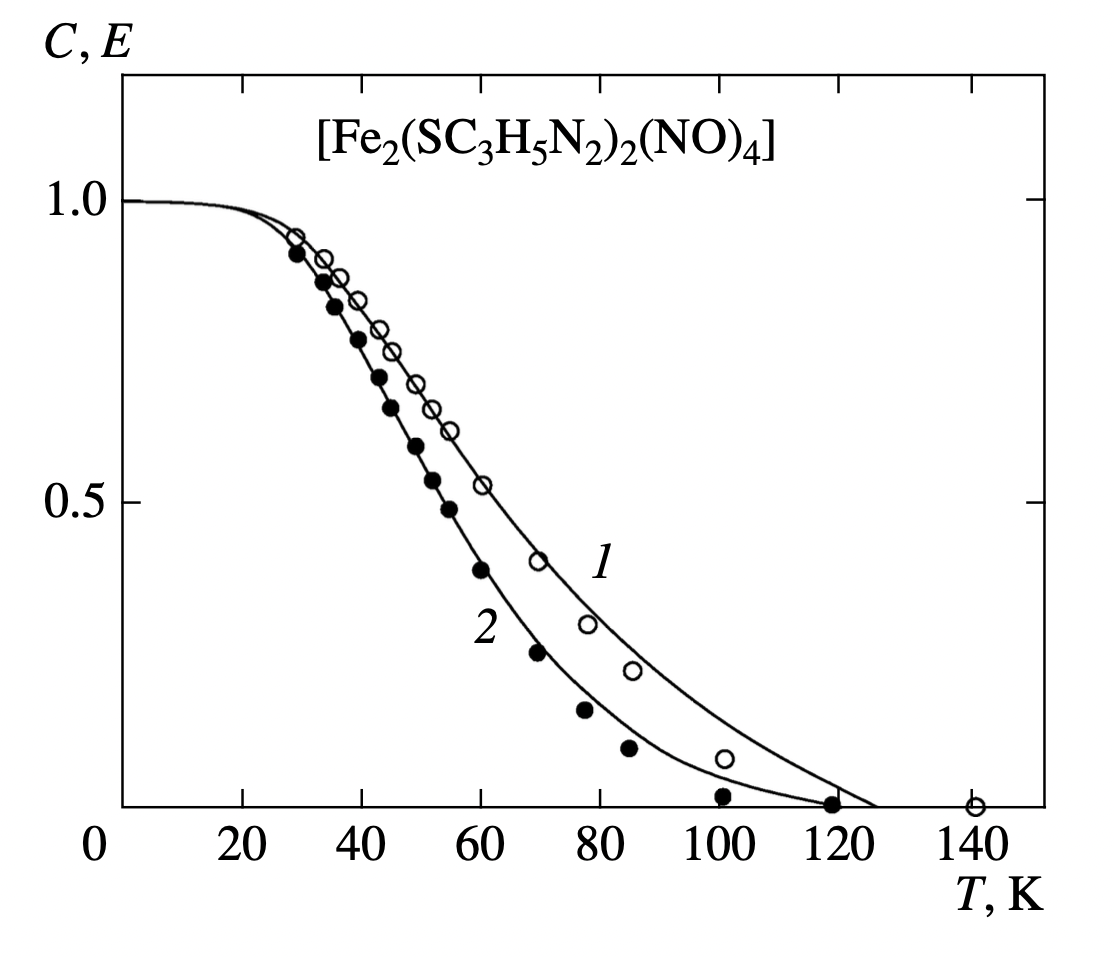
\includegraphics[width=0.5\textwidth]{Aldoshin2008-concurence-by-temp}
    \caption{
      Температурные зависимости согласованности (1) и запутанности (2) в     нитрозильном комплексе железа.
      Сплошные кривые 3 и 4 --- теоретические зависимости $C$ и $E$ соответственно.
    }
    \label{fig:concurence-temp-rcr}
\end{figure}

Позднее были найдены свидетели запутанности~\cite{Wootters1998, Bourennane2004, Kaszlikowski2008, Krammer2009, Bancal2011},
например, согласованность Вуттерса,
% Phys. Rev. A 85, 022321 (2012) Intorduction
а также критерии на основе неравенств ``сжимания'' спинов (spin-squeezing)~\cite{Sorensen2001, Durkin2005, Vitagliano2011, Duan2011}.
Согласованность является очень популярной мерой для количественной оценки двучастичных квантовых корреляций.
Она может быть определена как для чистых состояний,
так и для смешанных.
Вуттерс~\cite{Wootters1998} показал, что
%
\begin{equation}\label{eq:concurrence}
  C(\rho)
  = \max\left\{0, \lambda_1 - \lambda_2  - \lambda_3  - \lambda_4\right\}.
\end{equation}
%
Здесь $\lambda_1 \geq \lambda_2 \geq \lambda_3 \geq \lambda_4$ --- собственные числа матрицы
%
\begin{equation}
  R = \sqrt{\sqrt{\rho}\tilde{\rho}\sqrt{\rho}},
\end{equation}
где
%
\begin{equation}
  \tilde\rho = \p{\sigma_y \otimes \sigma_y}
    \rho^* \p{\sigma_y \otimes \sigma_y}.
\end{equation}
%
Также в общем случае смешанных двухкубитных систем запутанность $E(\rho)$ является функцией согласованности
\begin{equation}
  E(\rho) = H\p{\dfrac{1 + \sqrt{1 - C^2}}{2}},
\end{equation}
%
где $H(x)$ --- функция Шеннона~\cite{Shannon1948}
%
\begin{equation}
  H(x) = -x \log_2 x - (1 - x)\log_2(1 - x).
\end{equation}
%
Популярность критерия Вуттерса объясняется тем,
что выражение~(\ref{eq:concurrence}) может быть получено в аналитической форме.
В случае двухкубитной матрицы плотности, обладающей блочно-диагональной структурой вида
%
\begin{equation}
  \rho = \begin{pmatrix}
    u &  0  &  0  & 0 \\
    0 & x_1 &  w  & 0 \\
    0 &  w* & x_2 & 0 \\
    0 &  0  &  0  & v
  \end{pmatrix},
\end{equation}
%
согласованность определяется простой формулой:
%
\begin{equation}
  C = 2 \max\left\{0, |w| - \sqrt{uv} \right\}.
\end{equation}
%
В результате появляется возможность связать согласованность с реальными наблюдаемыми величинами.
Например, в работе~\cite{Aldoshin2012} была исследована температурная зависимость согласованности
в димере нитрозильного комплекса железа от магнитной восприимчивости антиферромагнитного димера (см. Рис.~\ref{fig:concurence-temp-rcr}).

Недавно другие подходы привели к критериям, которые могут быть оценены непосредственно по элементам матрицы плотности~\cite{Guhne2010, Huber2010}.
Дальнейшие работы по обнаружению многочастичной запутанности можно найти в работах~\cite{Li2010, Jungnitsch2011, Vicente2011, Huber2011} и в обзоре~\cite{Guhne2009}.
В частности, квадратичные неравенства типа Белла были получены Уффинком~\cite{Uffink2002, Nagata2002} в качестве тестов на многочастичную запутанность
и используются для классификации всех состояний $N$~кубитов на $N-1$~классов запутанности от двухчастично запутанного и до полностью запутанного
 ($N$-запутанного) состояния~\cite{Yu2003}.
Критерий на основе энтропии Реньи~\cite{Hosur2016, Fan2017}
является строгим свидетелем многочастичной запутанности для чистых состояний.
Энтропия Реньи может быть измерена экспериментально,
но для этого требуются ресурсы,
которые экспоненциально масштабируются с размером изучаемой системы,
а также возможность одночастичной адресации.

Хотя существуют и некоторые другие меры запутанных состояний, проблема классификации и количественного измерения
запутанности в целом всё ещё далека от полного
понимания~\cite{Guhne2009}.


\subsubsection{Оценка количества запутанных частиц в системе}
\label{sec:manyparticle-entanglement-criteria}
% Phys. Rev. A 85, 022321 (2012)  B. Multiparticle Entanglement
В то время как структура множества запутанных двучастичных квантовых состояний достаточно хорошо изучена,
о классификации и количественной оценке запутанности многочастичных квантовых состояний известно меньше\cite{Plbnio2007, Amico2008, Horodecki2009, Guhne2009}.
%
В данной работе будет подробно рассмотрен критерий,
использующий  неравенства Белла\cite{Bell1964} в терминах обобщенной меры информации $F$.

\begin{definition}\label{def:f}
Обобщенной мерой информации называется такая функция $F$,
которая удовлетворяет следующим свойствам:
\begin{enumerate}
  \item Значение меры объединения двух независимых подсистем --- это сумма значений меры, вычисленной для каждой подсистемы индивидуально:
  \begin{equation}\label{eq:f-additive-map}
    F(\rho_1 \otimes \rho_2 ,H_1 \otimes I_2 + I_1 \otimes H_2)
    = F_{1} (\rho_1, H_1) + F_{2} (\rho_2 , H_2),
  \end{equation}
  где $H_i$ --- это оператор, действующий на подсистему $\rho_i$,
  а $I_i$ --- это единичный оператор.

  \item Известна верхняя граница величины меры для системы $N$ частиц:
  \begin{equation}\label{eq:f-supremum}
    F \leq N^2.
  \end{equation}
\end{enumerate}
\end{definition}

\begin{definition}\label{def:rho-k-prod}
  Смешанное состояние $\rho_{k-\mathrm{prod}}$
является $k$-разделимым,
если оно может быть факторизовано на $l$ подсистем $\{\rho_i\}$ с размерами $\{N_i\}$,
где $\rho_i$ --- несепарабельное многокубитное состояние или однокубитное состояние,
и выполнено неравенство
\begin{equation}
  N > k \geq N_1 \geq N_2 \geq \dots \geq N_l \geq 1,
  \quad
  \sum_{i=0}^{l} N_i = N.
\end{equation}
\end{definition}
%
% Из свойств обобщенной меры информации $F$ следует,
% что для множества состояний $\mathcal{N} = \left\{\rho_{k-\mathrm{prod}}\right\}$ системы $N$ частиц%,
% % в которых максимальный размер несепарабельной подсистемы равен $k < N$,
% оценку (см. свойство \ref{eq:f-supremum}) ее верхней границы можно улучшить.
% Рассмотрим некоторое состояние $\rho_{k-\mathrm{prod}} \in \mathcal{N}$ ,
% которое может быть факторизованно на $l$ подсистем $\{\rho_i\}$,
% являющихся несепарабельными многокубитными состояниями или однокубитными состояниями, с размерами $\{N_i\}$, так что:
% \begin{equation}
%   N > k \geq N_1 \geq N_2 \geq \dots \geq N_l \geq 1,
%   \quad
%   \sum_{i=0}^{l} N_i = N.
% \end{equation}
%
Из свойств обобщенной меры информации $F$ следует,
что для произвольной $k$-частично разделимой матрицы плотности $\rho_{k-\mathrm{prod}}$~(см.~определение~\ref{def:rho-k-prod})
% что для множества состояний $\mathcal{N} = \left\{\rho_{k-\mathrm{prod}}\right\}$
% системы $N$ частиц,
оценку~(см.~свойство~\ref{eq:f-supremum}) ее верхней границы можно улучшить.
Используя свойство аддитивности~(\ref{eq:f-additive-map}) меры $F$,
можно оценить сверху величину обобщённой информации для каждой подсистемы отдельно
%
\begin{equation}\label{eq:f-subsystems}
  F(\rho_{k-\mathrm{prod}}) =
  F(\rho_1) + F(\rho_2) + \dots + F(\rho_l)
  \leq N^2_1 + N^2_2 + \dots + N^2_l.
\end{equation}
%
Максимальное значение правой части выражения~(\ref{eq:f-subsystems}) достигается,
когда система состоит из $m = \left[\frac N k \right]$ подсистем размера $k$
и одной подсистемой с остатком
%
\begin{equation}\label{eq:f-worse-distribution}
  \sup_{\left\{\rho_{k-\mathrm{prod}}\right\}}
    \left(N^2_1 + N^2_2 + \dots + N^2_l\right)
  = \underbrace{
    k^2 + k^2 + \dots + k^2
    }_{m = \left[\frac N k \right] \, \mbox{раз}}
    + \underbrace{(N-km)^2}_{\mbox{остаток}}.
\end{equation}
%
Докажем это утверждение.
Рассмотрим два последних слагаемых выражения~(\ref{eq:f-worse-distribution}) и предположим, что
%
\begin{multline}\label{eq:n-i-distribution-inequality}
  k^2 + (N-km)^2 < (k - 1)^2 + (N-km + 1)^2 \\
  = k^2 + (N-km)^2
    - 2\p{k - 1 \underbrace{(N-km)}_{ = \phi, \, 0 \leq \phi < 1}} \\
  = k^2 + (N-km)^2 - 2(k - 1 - \phi).
\end{multline}
%
Неравенство~(\ref{eq:n-i-distribution-inequality}) нарушается при $k \geq 2$. Противоречие.
Правая часть выражения~(\ref{eq:f-entangled}) не превосходит $N^2$.
С учетом
$m = \left[\frac{N}{k}\right] = \frac{N}{k} -\phi$ ($0 \leq \phi < 1$)
получаем
%
\begin{equation}
  k^2m + \p{N-km}^2
  = k^2\left(\frac{N}{k} - \phi\right) + (N - N +k\phi)^2  < kN \leq N^2.
\end{equation}
%
Объединяя выражения~(\ref{eq:f-subsystems})~и~(\ref{eq:f-worse-distribution}),
получаем верхнюю границу величины меры $F$ для $k$-разделимой матрицы плотности $\rho_{k-\mathrm{prod}}$ системы $N$
%
\begin{equation}\label{eq:f-entangled}
  F\p{\rho_{k-\mathrm{prod}}}
  \leq F_{N, k-\mathrm{prod}}
  = \left[ \frac N k \right] k^2 + \left(N - k \left[ \frac N k \right]\right)^2.
\end{equation}
%


Для примера ниже приведены значения $F_{N, k-\mathrm{ent}}$
для систем $N = 2, 3, 4, 5$ частиц:
\begin{itemize}
  \item[(1)]
    $F_{2, 1-\mathrm{prod}}= 2$,
    $F_{2, 2-\mathrm{prod}}= 4$;
  \item[(2)]
    $F_{3, 1-\mathrm{prod}}= 3$,
    $F_{3, 2-\mathrm{prod}}= 5$,
    $F_{3, 3-\mathrm{prod}}= 9$;
  \item[(3)]
    $F_{4, 1-\mathrm{prod}}= 4$,
    $F_{4, 2-\mathrm{prod}}= 8$,
    $F_{4, 3-\mathrm{prod}}= 10$,
    $F_{4, 4-\mathrm{prod}}= 16$;
  \item[(4)]
    $F_{5, 1-\mathrm{prod}}= 5$,
    $F_{5, 1-\mathrm{prod}}= 9$,
    $F_{5, 1-\mathrm{prod}}= 13$,
    $F_{5, 1-\mathrm{prod}}= 17$,
    $F_{5, 1-\mathrm{prod}}= 25$.
\end{itemize}


\begin{theorem}\label{th:entanglement-criteria}
  Состояние $\rho$ является $k$-частично запутанным $\rho_\mathrm{k-ent}$,
  если оно удовлетворяет неравенству
  \begin{equation}\label{eq:entanglement-criteria}
    F_{N, (k-1)-\mathrm{prod}} < F(\rho),
  \end{equation}
\end{theorem}
\textbf{Доказательство.}
Пусть $F_{N, (k-1)-\mathrm{prod}} < F(\rho)$ выполнено,
но состояние $\rho$ не является $k$-частично запутанным.
Тогда согласно определению~\ref{def:manyparticle-entanglement} максимально возможный размер несепарабельной подсистемы равен  $k-1$,
и,
согласно определению~\ref{def:rho-k-prod} состояние $\rho$ является $k-1$-частично разделимым.
Согласно выражению~\ref{eq:f-entangled}, величина обобщенной информации $k-1$-частично разделимой матрицы плотности не может превышать $F(\rho) \leq F_{N, (k-1)-\mathrm{prod}}$.
Противоречие.

В настоящее время признано,
что большинство физических процессов в природе можно сформулировать в терминах обработки информации,
и концепция информации может быть центральной для понимания квантовой теории\cite{Zurek1990, Summhammer1994, Frieden2004}.
В частности, в качестве обобщённой информационной меры в квантовой теории информации могут выступать
\begin{enumerate}
  \item Косая информация Вигнера-Янасе\cite{Zeqian2005},
  \item Квантовая информация Фишера\cite{Hyllus2012}.
\end{enumerate}

% В частности, было показано\cite{Garttner2018},
% что нижняя граница квантовой информации Фишера соответствует
% второму моменту спектра интенсивностей многоквантовых когерентностей.
  \section{Косая информация Вигнера-Янасе}
% история
% определение
% применение
% свойства
% формула
% связь c информацией Фишера
% связь со вторым моментом

% 10.1103/PhysRevLett.91.180403 Inro
% В исследовании измерения квантовомеханических операторов Вигнер показал, что наблюдаемые, которые не коммутируют с аддитивной сохраняющейся величиной, труднее измерить, чем те, которые коммутируют с сохраняющейся величиной; то есть, наличие закона сохранения накладывает ограничение на измерение наблюдаемых, которые несовместимы (не коммутируют) с сохраняющейся величиной [1,2]. Араки и Янасе строго установили, что наблюдаемые величины, не совпадающие с сохраняющейся величиной, не могут быть измерены точно (в смысле фон Неймана), возможно только приближенное измерение, и существует компромисс между "размером" измерительного прибора и точностью измерения [3,4]. Это составляет знаменитую теорему Вигнера-Араки-Янасе, которая накладывает принципиальное ограничение на измерение квантовомеханических наблюдаемых. Эта теорема в дальнейшем исследовалась многими авторами [5-9].
% Cледовательно наблюдаемые величины, 
% которые коммутируют с аддитивными сохраняющимися величинами 
% (энергия, компоненты линейного и углового моментов, электрический заряд), 
% могут быть измерены с помощью микроскопических аппаратов, 
% а те, которые не коммутируют с этими величинами, требуют для своего измерения макроскопических систем\cite{Wigner1960}.

% 
%Согласно квантовомеханической теории, 
% екоторые наблюдаемые величины могут быть измерены гораздо легче, чем другие:

Араки и Янасе строго установили, что наблюдаемые величины, 
которые не являются интегралами движения, 
не могут быть измерены точно (в смысле фон Неймана), 
и возможно только приближенное измерение. 
Согласно знаменитой теореме Вигнера-Араки-Янасе, которая накладывает принципиальное ограничение на измерение квантовомеханических наблюдаемых,
существует компромисс между ``размером'' измерительного прибора и точностью измерения\cite{Araki1961, Ozawa1991, Ozawa2002a, Ozawa2002b, Matsumoto1993, Kakazu3469}.
Наблюдаемые величины, 
которые коммутируют с аддитивными сохраняющимися величинами 
(энергия, компоненты линейного и углового моментов, электрический заряд), 
могут быть измерены с помощью микроскопических аппаратов; 
те же, которые не коммутируют с этими величинами, требуют для своего измерения макроскопических систем\cite{Wigner1960}.
Отсюда возникает проблема определения меры наших знаний относительно последних. 

% Theoretical and Mathematical Physics, 202(1): 104–111 (2020)
Косая информация\cite{Wigner1963} была введена Вигнером и Янасе 
в контексте квантовых измерений в качестве меры информации,
содержащейся в векторе квантового состояния, лежащего под углом по отношению к наблюдаемой $A$.
\begin{equation}\label{eq:wyi}
  I_{WY}(\rho, A)
  = -\frac{1}{2} Tr([\sqrt{\rho}, A])^2
  = Tr(\rho A^2) - Tr(\sqrt \rho A \sqrt \rho  A ).
\end{equation}    
% 
В частности, если $\rho = \ket{\psi}\bra{\psi}$ чистое состояние, тогда 
%
\begin{equation}
  I_{WY}(| \psi \rangle, A)
  = \langle \psi | A^2 | \psi \rangle - \langle \psi | A| \psi \rangle ^2
\end{equation}
  
Косая информация Вигнера-Янасе существенно отличается от энтропии фон Неймана \cite{Wigner1960, Lieb1973prl, Lieb1973, Wehrl1978}, 
но глубоко связана с ней.
Энтропия, как ее обычно определяют, является мерой нашего незнания\cite{Weaver1949}.
Это мера, в которой знания о любой наблюдаемой величине находятся в одном ряду.
С точки зрения энтропии информационное содержание всех чистых состояний,
которые могут быть описаны одним вектором состояния, одинаково. 
Это неверно для косой информации Вигнера-Янасе.
В отличие от вектора консервативной величины наблюдаемой $A$, 
вектор состояния, лежащего наклонно к наблюдаемой $A$, содержит информацию.

Позднее было признано, что косая информация, 
помимо своего изначального значения как меры информационного содержания состояний,
допускает также несколько интерпретаций, 
носящих более физический и теоретико-информационный характер. 
Например, Шунь Лун Ло показал\cite{Luo2003, Luo2005, Luo2005pra, Luo2006, Luo2017} , 
что косую информацию Вигнера-Янасе можно интерпретировать
как квантовую неопределенность наблюдаемой $A$ для квантового состояния $\rho$.

Интригующей и тонкой особенностью косой информации является использование в ней квадратного корня из оператора плотности квантового состояния. 
Тем не менее популярность получили и естественные модификации косой информации Вигнера-Янасе, 
в которых нет корня из оператора плотности.
Например, величина
%
\begin{equation}\label{eq:wyi-modification-l}
  L(\rho, A)
  = -\frac{1}{2} Tr([\rho, A])^2.
\end{equation} 
%
Значительным преимуществом величины $L(\rho, A)$ в сравнении с косой информацией является возможность ее измерения экспериментально [12]. 
В [16] было показано, 
что $L(\rho, A)$ можно измерить в "интерферометрической" установке (an interferometric setup) путем выполнения только двух программируемых измерений независимо от размерности квантовой системы.
Однако существует проблема зависимости $L(\rho, A)$ от характеристик вспомогательной системы, как было отмечено в [24].
С помощью сравнения косой информации с некоторыми ее естественными модификациями были раскрыты\cite{Luo2020} математические, 
а также физические причины использования квадратного корня. 

% Skew information has many nice properties and interpretations that make it useful in quantum information theory[1], [8].
В настоящее время косая информация Вигнера-Янасе нашла много применений в квантовой теории информации[1], [8]. 
% For example, skew information can be used to construct measures of quantum correlations [9]–[11],
% to quantify quantum coherence [12]–[15], to quantify asymmetry [15], and so on.
Например, информация о перекосе может быть использована для построения мер квантовых корреляций [9]-[11], 
для количественной оценки квантовой когерентности [12]-[15], 
для количественной оценки асимметрии [15] и так далее.
% It has also been used to study quantum phase transitions [16]–[20], uncertainty relations [6], [21]–[23], et cetera.
Она также использовалась для изучения квантовых фазовых переходов [16]-[20], соотношения неопределенностей [6], [21]-[23] и т.д.

Особенно нужно отметить, 
что косая информация удовлетворяет свойствам из определения~(\ref{def:f}), 
и, cледовательно, может быть использована для оценки количества запутанных частиц в системе. 

% Chen2005


% ---- PRA
Тем не менее полноценное исследование многочастичной запутанность в системе
требует разработки соответствующих экспериментальных методов. 
Основной недостаток квантовой информации Вигнера-Янасе заключается в том, 
что эта величина не могла быть измерена экспериментально, 
в отличии информации Фишера\cite{Garttner2018}. 
Одним из главных достижений данной работы является преодоление этого препятствия. 
В Главе~\ref{chapter:wyi-mesuarement} представлена теория экспериментального метода определения величины косой информации Вигнера-Янасе 
в спиновой системе с диполь-дипольным взаимодействием в многоквантовом эксперименте ЯМР. 
Оказывается,
что в этом случае косая информация Вигнера-Янасе тоже связана со значением 
второго момента спектра интенсивностей многоквантовых когерентностей в системе.

% It is not a random magic because skew information may be identifier as a paradigmatic version of quantum Fisher information.
% % the statistical idea underlying the skew information is the Fisher information in the theory of statistical estimation.
  \section{Информация Фишера}
% история
% oпределение
% применение
% вывод
% свойства
% формула
% связь со вторым моментом

% PETZ2011 https://doi.org/10.1142/9789814338745_0015
Оценка параметров вероятностных распределений является одной из самых основных задач в теории информации
и она была обобщена на квантовый режим\cite{Helstrom1976, Holevo1982}, поскольку описание квантового измерения является по сути вероятностным.

\subsection{Классическая информация Фишера}
Классическая информация Фишера является мерой того,
как быстро изменяется распределение информации при изменении некоторого параметра.

\begin{definition}\label{def:fisher-information}
 Информация Фишера --- это математическое ожидание квадрата относительной скорости изменения условной плотности вероятности,
 при изменении некоторого параметра.
\end{definition}
%
\begin{equation}\label{eq:fisher-information}
  F_c({\theta})=
      \sum_x{{P}(x,\theta)}
          \left[\frac{1}{P(x,\theta)}
     \frac{d}{d\theta}
  {P(x,\theta)}\right]^2
\end{equation}
%
Важно отметить,
что квадрат играет ключевую роль в определении информации Фишера
и отказаться от него невозможно:
%
\begin{equation}
    \label{eq:2}
        \sum_x{{P}(x,\theta)}
            \frac{1}{P(x,\theta)}
                \frac{dP(x,\theta)}{d\theta} =
                    \sum_x\frac{{dP}(x,\theta)}{d\theta} =
                \frac{d}{d\theta}\sum_x{{P}(x,\theta)} =
            \frac{d}{d\theta}1 =
            0
\end{equation}

Выражение~(\ref{eq:fisher-information}) для классической информации фишера, можно переписать через математическое ожидание:
\begin{multline}
    \label{eq:17}
        F_c(\theta) =
            \sum_x P(x, \theta)\left[\frac{1}{P(x,\theta)}\frac{d}{d_\theta} P(x, \theta)\right]^2 \\
                = \sum_x P(x,\theta)\left[\frac{d}{d_\theta}
                    \ln P(x,\theta \right]^2 \\
                    \Rightarrow E
                \left[\left(\frac{d}{d_\theta}\ln f(X,\theta)\right)^2
            \right]
\end{multline}
%
В случае, если $f(X,\theta)$ дважды дифференцируема по $\theta$,
выражение~(\ref{eq:17}), можно упростить и записать в виде
%
\begin{equation}\label{eq:18}
  F_c(\theta) = -E \left[\frac{\partial^2}{\partial \theta^2} \ln f(X,\theta)\right].
\end{equation}
%
Для доказательства выражения~(\ref{eq:18}),
продифференцируем выражение под оператором математического ожидания:
%
\begin{multline}
    \label{eq:19}
        \frac{\partial^2}{\partial \theta^2}\ln f(X,\theta) =
            \frac{\partial}{\partial \theta}\left(\frac{1}{f(X,\theta)}
                \frac{\partial f(X,\theta)}{\partial \theta} \right) \\
            = \frac{1}{f(X,\theta)}\frac{\partial^2 f(X,\theta)}{\partial \theta^2} -
        \left(\frac{1}{f(X,\theta)} \frac{\partial f(X,\theta)}{\partial \theta}
    \right)^2
\end{multline}
%
Покажем,
что математическое ожидание первого слагаемого выражения~(\ref{eq:19}) тождественно равно нулю:
%
\begin{multline}
    \label{eq:20}
        E\left[\frac{1}{f(X,\theta)}
            \frac{\partial^2 f(X,\theta)}{\partial \theta^2}\right] =
                \int f (X,\theta) \frac{1}{f(X,\theta)}
                    \frac{\partial^2 f(X, \theta)}{\partial \theta^2}dx \\
                        = \int \frac{\partial^2 f(X,\theta)}{\partial \theta^2}dx =
                    \frac{\partial^2}{\partial \theta^2} \int f(X,\theta)dx
                = \frac{\partial^2}{\partial \theta^2}1 \equiv 0
\end{multline}
%
Отсюда следует~(\ref{eq:18}).
Приведенное доказательство справедливо при условии регулярности $f(X,\theta)$.


%  (Cramer-Rao bound)
Информация Фишера играет важную роль в задачах оценки параметров.
Оказалось, что обратная информация Фишера является нижней границей дисперсии при оценке параметров, называемой границей Крамера-Рао.
Докажем это утверждение.
%
Исходим из тождества:
%
\begin{multline}
    \label{eq:21}
        E[\hat{\theta}(X) - \theta] =
            \int(\hat{\theta}(x) - \theta)f(x,\theta)d\theta \\
                = \int\theta(x)f(x,\theta)dx - \int f(x,\theta)dx \equiv 0
\end{multline}
%
Формально это выражение может быть записано следующим образом
%
\begin{multline}
    \label{eq:22}
        0 = \frac{\partial}{\partial \theta}
            \int(\hat{\theta}(X) - \theta)f(x,\theta)dx \\
                = \int(\hat{\theta}(X) - \theta)
            \frac{\partial f(X, \theta)}{\partial \theta}dx -
        \int f(x,\theta)dx
\end{multline}
%
Поскольку $\frac{\partial f}{\partial \theta} = f(x,\theta)
    \frac{\partial \ln f(x,\theta)}{\partial \theta}$,
~(\ref{eq:22}) можно переписать в виде
%
\begin{equation}
    \label{eq:23}
        \int(\hat{\theta}(X) - \theta)
            f(x,\theta) \frac{\partial \ln f(x,\theta)}
        {\partial \theta}dx = 1
\end{equation}
%
Выражение~(\ref{eq:22}) перепишем в форме:
%
\begin{equation}
    \label{eq:24}
        \int \left[\hat{\theta}(X-\theta)\Large \sqrt{\mathstrut f(x,\theta)}\right]
            \left[\Large\sqrt{\mathstrut f(x,\theta)}
                \frac{\partial \ln f(x,\theta)}{\partial \theta}\right]dx = 1
\end{equation}
%
Применяя к~(\ref{eq:24}) неравенство Коши-Шварца, получаем:
%
\begin{multline}
    \label{eq:25}
        1 = \left(\int \left[(\hat{\theta}(X)-\theta)
            \Large \sqrt{\mathstrut f(x,\theta)}\right]
                \left[\Large \sqrt{\mathstrut f(x,\theta)}
                    \frac{\partial \ln f(x,\theta)}{\partial \theta} \right]
                \right)^2 \\
                \leq \int
            \underbrace{[(\hat{\theta}(X) - \theta)^2 f(x,\theta)]}_{Var(\hat{\theta}(X))}dx
        \underbrace{\int\left[f(x,\theta)\left(\frac{\partial \ln f(x,\theta)}
    {\partial \theta}\right)^2 \right]dx}_{F_c(\theta)}
\end{multline}
%
Отсюда получаем выражение для границы Крамера-рао:
%
\begin{equation}
    \label{eq:26}
        Var(\hat{\theta}(X)) \geq 1/{F_c (\theta)}
\end{equation}




\subsection{Квантовая информация Фишера}
\label{sec:quantum-fisher-information}
\begin{definition}\label{def:quantum-fisher-information}
  Квантовая информация Фишера~\cite{liu2014} показывает,
  как быстро изменяется квантовое состояние,
  определяемое матрицей плотности, при изменении некоторого параметра.
\end{definition}
Переход к квантовой информации Фишера соответствует обычной процедуре перехода от классических величин к квантовым.
Квантовая информация Фишера определяется по формуле:
%
\begin{equation}
    \label{eq:3}
        F_Q (\rho_\theta) =
            Tr[\rho_\theta, L^2_\theta],
\end{equation}
%
где $\rho_\theta$ --- это матрица плотности системы, зависящая от параметра $\theta$, а симметричный оператор логарифмической производной $L_\theta$, определяется из уравнения:
%
\begin{equation}
    \label{eq:4}
        \frac{\partial\rho_\theta}{\partial\theta} =
            \frac{1}{2}
                \left(L_\theta \rho_\theta +
                \rho_\theta L_\theta
            \right).
\end{equation}
%
В классическом случае, когда $\left[L_\theta, \rho_\theta \right]$ = 0 из ~(\ref{eq:4}) находим,
что ${L_\theta\sim\frac{\partial\ln\rho_\theta}{\partial\theta}}$,
и формула~(\ref{eq:3}) дает результат, совпадающий с~(\ref{eq:fisher-information}).
%
Зависимость матрицы плотности системы от параметра $\theta$ может быть введена в систему разными способами.
Мы рассмотрим случай, когда эта зависимость определяется унитарной эволюцией.
%
\begin{equation}
    \label{eq:5}
        \rho_\theta =
            e^{iH\theta}
        \rho e^{-iH\theta},
\end{equation}
%
где $\rho$ --- произвольная матрица плотности, $H$ --- эрмитов гамильтониан системы.
Такой способ введения параметра отвечает условиям многоквантовой спектроскопии ЯМР.
В этом случае:
%
\begin{equation}
    \label{eq:6}
        \frac{\partial\rho_\theta}{\partial\theta} =
            iH\rho_\theta - i\rho_\theta H =
        i \left[H,\rho_\theta \right]
\end{equation}
%
Дальнейшие вычисления проведем в базисе, диагонализирующем матрицу плотности $\rho$ $\left(\rho =\sum\limits_{k} \lambda_k |k\rangle  \langle k| \right)$.
Используя уравнения ~(\ref{eq:4}) и ~(\ref{eq:6}) получаем
%
\begin{multline}\label{eq:7}
    i \left[H,\rho_\theta \right]_{jk} =
        \frac{1}{2} \sum_e \left(L_\theta \right)_{je}
            \left(\rho_\theta \right)_{ek} +
                \frac{1}{2} \sum_e \left(\rho_\theta \right)_{je}
                    \left(L_\theta \right)_{ek} =\\
                \frac{1}{2}\left(L_\theta \right)_{{jk}^{\lambda} k} +
            \frac{1}{2}\lambda_j \left(L_\theta \right)_{jk} =
    \frac{1}{2} \left(\lambda_k + \lambda_j \right)
    \left(L_\theta \right)_{ik}
\end{multline}
%
Таким образом,
 %
\begin{equation}
    \label{eq:8}
        \left(L_\theta \right)_{jk} =
            \frac{2i\left[H,\rho_\theta \right]_{jk}}{\lambda_k + \lambda_j},
\end{equation}
%
Умножим теперь~(\ref{eq:6}) на $L_\theta$ и возьмем след:
%
\begin{equation}
    \label{eq:9}
        Tr\Bigg\{L_\theta \frac{\partial \rho_\theta}{\partial \theta} \Bigg\} =
            \frac{1}{2} Tr\left(L^2_\theta \rho_\theta \right) +
                \frac{1}{2} Tr\left(L_\theta \rho_\theta L_\theta \right) =
            Tr \left(L^2_\theta \rho_\theta \right) =
        F_Q \left(\rho_\theta, H \right)
\end{equation}
%
Далее
%
\begin{equation}
    \label{eq:10}
        \left[H, \rho_\theta \right]_{jk} = \sum_e H_{je}
            \left(\rho_\theta \right)_{ek} -
                \sum_e \left(\rho_\theta \right)_{jl}H_{ek} =
            H_{jk}\lambda_k - H_{jk}\lambda_j =
        \left(\lambda_k - \lambda_j \right) H_{jk}.
\end{equation}
%
Теперь
%
\begin{equation}
    \label{eq:11}
        F_Q \left(\rho_\theta, H \right) =
            \sum_{j,k}\frac{2i\left[H,\rho_\theta \right]_{jk}}
                {\lambda_k + \lambda_j}
                    i \left[H, \rho_\theta \right]_{kj} =
                2\sum_{j,k} \frac{\left(\lambda_j - \lambda_k \right)^2}
            {\lambda_j + \lambda_k}
        \left| \langle j|H|k \rangle \right|^2
\end{equation}
%
В итоге, получаем основную формулу для квантовой информации Фишера
%
\begin{equation}\label{eq:quantum-fisher-information}
        F_Q \left(\rho_\theta, H \right) =
            2\sum_{j,k} \frac{\left(\lambda_j - \lambda_k \right)^2}
                {\lambda_j + \lambda_k}
            \left| \langle j|H|k \rangle \right|^2
\end{equation}

Покажем, что квантовая информация Фишера удовлетворяет свойствам~(\ref{def:f}),
и, следовательно, может быть использована для оценки количества запутанных частиц.
Квантовая информации Фишера в сепарабельной системе с матрицей плотности $\rho = \rho_1 \otimes \rho_2$ удовлетворяет свойству аддитивности:
%
\begin{equation}\label{eq:31}
  F_Q(\rho_1 \otimes \rho_2 ,H_1 \otimes I_2 + I_1 \otimes H_2) =
      F_{Q1} (\rho_1, H_1) + F_{Q2} (\rho_2 , H_2)
\end{equation}
%
Также, величина квантовой информации Фишера в системе из $N$ частиц
ограничена сверху:
%
\begin{equation}\label{eq:33}
  F_Q \leq N^2
\end{equation}
%
Докажем утверждение~(\ref{eq:33}).
Исходим из формулы
%
\begin{equation}
    \label{eq:34}
        F_Q = 2\sum_{\substack{j,k \\ \lambda_j + \lambda_k \neq 0}}
            \frac{(\lambda_j - \lambda_k)^2}{\lambda_j + \lambda_k}
                \left| \langle j|H|k \rangle \right|^2
\end{equation}
%
Убедимся, что
\begin{equation}
  \frac{(\lambda_j - \lambda_k)^2}{\lambda_j +\lambda_k} \leq 1.
\end{equation}
Неравенство
\begin{equation}
  \lambda_j + \lambda_k \geq \lambda^2_j +\lambda^2_k
\end{equation}
верно, т.к. $0\leq \lambda_j \leq 1$, $0\leq \lambda_k \leq 1$.
%
Далее
\begin{equation}
\lambda_j + \lambda_k \geq\lambda^2_j +\lambda^2_k \geq \lambda^2_j +\lambda^2_k - 2\lambda_j \lambda_k = (\lambda_j - \lambda_k)^2 \Rightarrow 1 \geq \frac{(\lambda_j - \lambda_k)^2}{\lambda_j + \lambda_k}.
\end{equation}
%
Гамильтониан Н в~(\ref{eq:34}) безразмерный.
Предполагаем, обезразмеривание проиведено на максимальный модуль недиагонального элемента гамильтониана Н (все элементы поделены на $\left| \langle j|H|k \rangle \right| + \left| \langle k|H|j \rangle \right| = 2\left| \langle j|H|k \rangle \right|$,)
%
тогда
%
\begin{equation}
    \label{eq:35}
        \left| \langle j|H|k \rangle \right| \leq 1/2
\end{equation}
%
В итоге получаем оценку сверху для квантовой информации Фишера:
%
\begin{equation}
    \label{eq:36}
        F_Q = 2\sum_{\substack{j,k \\ \lambda_j + \lambda_k \neq 0}}
            \frac{(\lambda_j - \lambda_k)^2}{\lambda_j + \lambda_k}
                \left| \langle j|H|k \rangle \right|^2
            \leq 2\sum^N_{\substack{j,k \\ \lambda_j + \lambda_k \neq 0}} \left| \langle j|H|k \rangle \right|^2
            \leq N^2
\end{equation}

  \section{Сравнение информаций Фишера и Вигнера-Янасе}
\label{sec:qfi-wyi-comparison}
%
Квантовая информация Фишера~(см. раздел~\ref{sec:quantum-fisher-information})
и косая информация Вигнера-Янасе~(см. раздел~\ref{sec:skew-wigner-yanase-information})
удовлетворяют свойствам обобщенной информации~(см. определение~\ref{def:f}).
Следовательно, обе информации могут быть использованы для исследования многочастичной запутанности.
Для того чтобы прояснить связь между этим фундаментальными мерами,
в этом разделе будет проведено сравнение величин этих информаций для произвольной матрицы плотности $\rho$
и оператора проекции полного углового спинового момента на ось~$z$
в качестве наблюдаемой.

Матрица плотности $\rho$ в диагонализирующем ее базисе,
имеет вид
%
\begin{equation}
  \rho = \sum\limits_i \lambda_i \ket{i}\bra{i},
\end{equation}
%
где $\lambda_i$ --- собственное значение,
а $\ket{i}$ соответствующий собственный вектор.
%
В этом базисе косая информация Вигнера-Янасе может быть записана как:
%
\begin{multline}\label{eq:wyi-via-lambda}
  I_\mathrm{WY}(\rho, I_z)
  = -2 \tr{[\rho, I_z]^2}
  = -2 \sum\limits_{i,k} [\sqrt{\rho}, I_z]_{ik} [\sqrt{\rho}, I_z]_{ki}
  \\
  = -2 \sum\limits_{i,k}
    \p{\sqrt{\lambda_i}(I_z)_{ik} - (I_z)_{ik} \sqrt{\lambda_k}}
    \p{\sqrt{\lambda_k}(I_z)_{ki} - (I_z)_{ki} \sqrt{\lambda_i}}
  \\
  = -2 \sum\limits_{i,k} \p{
    \sqrt{\lambda_i}\sqrt{\lambda_k}
    - \lambda_k
    - \lambda_i
    + \sqrt{\lambda_k}\sqrt{\lambda_i}
    }
    (I_z)^2_{ki}
  \\
  = 2 \sum\limits_{i,k} \p{\sqrt{\lambda_i} -\sqrt{\lambda_k}}^2
    \left| \bra{i} I_z \ket{k} \right|^2
\end{multline}
%
В свою очередь квантовая информации Фишера может быть выражена как
%
\begin{multline}\label{eq:qfi-via-wyi}
  I_\mathrm{F}(\rho, I_z)
  = 2 \sum\limits_{i,k}
    \dfrac{\p{\lambda_i - \lambda_k}^2}{\lambda_i + \lambda_k}
    \left| \bra{i} I_z \ket{k} \right|^2
  \\
  = 2 \sum\limits_{i,k}
    \dfrac{
      \p{\sqrt{\lambda_i} +\sqrt{\lambda_k}}^2
    }{
      \lambda_i + \lambda_k
    }
    \p{\sqrt{\lambda_i} -\sqrt{\lambda_k}}^2
    \left| \bra{i} I_z \ket{k} \right|^2
  \\
  = 2 \sum\limits_{i,k}
    \p{1 + \dfrac{2\sqrt{\lambda_i}\sqrt{\lambda_k}}{\lambda_i + \lambda_k}}
    \p{\sqrt{\lambda_i} -\sqrt{\lambda_k}}^2
    \left| \bra{i} I_z \ket{k} \right|^2
  \\
  = 2 \sum\limits_{i,k} \p{1 + \alpha_{ik}}
  \p{\sqrt{\lambda_i} -\sqrt{\lambda_k}}^2
  \left| \bra{i} I_z \ket{k} \right|^2,
\end{multline}
%
где $\alpha_{ik} = \dfrac{2\sqrt{\lambda_i}\sqrt{\lambda_k}}{\lambda_i + \lambda_k}$.
Так как $ 0 \leq \alpha_{ik} \leq 1$
из выражений~(\ref{eq:qfi-via-wyi})~и~~(\ref{eq:wyi-via-lambda}) следует, что
%
\begin{equation} \label{eq:qfi-wyi-inequality}
    I_{WY}\left(\rho, I_z\right)
    \leq I_F\left(\rho, I_z\right)
    \leq 2I_{WY}\left(\rho, I_z\right).
\end{equation}


  % \section{Методы исследования квантовых систем}
% Ионны в ловышках, сверхпроводящие кубиты и прочее.
  \section{Многоквантовая спектроскопия ЯМР}
% JMR-2020
Среди различных модельных физических систем,
рассматриваемых для реализации устройств и систем квантовой обработки информации,
ядерные спины обладают исключительной изоляцией от внешней среды
и широкими возможностями для манипулирования радиочастотными импульсами.
Многоквантовая (MK) спектроскопия ЯМР~\cite{Baum1985} позволяет создавать многоквантовые состояния,
а также экспериментально отслеживать процесс их релаксации.
%Одним из таких экспериментов является многоквантовый (МК) ЯМР в системах спинов,
%связанных прямым диполь-дипольным взаимодействием (DDI).
Приложения МК спектроскопии ЯМР включают широкий спектр неорганических и органических твердых тел и жидких кристаллов [2].
МК спектроскопия ЯМР может использоваться для решения вопроса о распределении атомов в материалах
и особенно хорошо подходит для анализа сложных по составу и неупорядоченных систем [3-5].
МК ЯМР может быть использован для изучения декогеренции в системах,
состоящих из большого числа коррелированных спинов [6,7],
что открывает возможности для установления связи между числом частиц и скоростью декогеренции [6,8].
Метод позволяет следить за распространением корреляций [1,9]
и наблюдать явления локализации в системах многих тел [10,11].
Скорость распространения может быть описана через корреляторы класса ``out-of-time ordered correlations''~(OTOCs),
которые связаны с распределением интенсивности когерентностей МК ЯМР [12,13].

% Многоквантовая спектроскопия ЯМР служит эффективным методом для изучения распределения ядерных спинов в жидких кристаллах [2],
% в простых органических соединениях [1],
% в аморфном гидрированном кремнии [3] и т.д.
% Многоквантовый ЯМР успешно применяется [4, 5] для исследования размеров спиновых кластеров
% при их росте в процессе облучения спиновой системы радиочастотными (РЧ) импульсами на подготовительном периоде многоквантового эксперимента ЯМР [1].
% Недавно уникальные возможности многоквантового ЯМР были использованы [6, 7] для определения зависимости скорости декогеренции сильно коррелированных спиновых состояний от числа коррелированных спинов.

Многоквантовая динамика ядерного магнитного резонанса (ЯМР) является основой многоквантовой спектроскопии ЯМР~\cite{Baum1985}.
В обычных экспериментах ЯМР происходят лишь переходы между зеемановскими уровнями
с изменением проекции спинового момента на направление внешнего магнитного поля на $\pm 1$.
В результате основные наблюдаемые (например, спад свободной индукции) определяются относительно небольшим количеством отличных от нуля элементов матрицы плотности.
В многоквантовых экспериментах ЯМР,
где в принципе возможны переходы между любыми уровнями,
состояние спиновой системы определяется всеми элементами матрицы плотности.
Таким образом, информационный ресурс многоквантового ЯМР превосходит ресурс обычного ЯМР.

Теоретическое описание многоквантовой динамики ЯМР является сложной задачей, которая сводится к анализу многочастичную и многоквантовой системы. Матрицу плотности системы в многоквантовом эксперименте ЯМР можно представлять суммой членов, каждый из которых содержит тензорные произведения односпиновых операторов
(например, для $k$~-спина это $I_{kz}$,
$I_k^+ = I_{kx} + iI_{ky}$, $I_k^+ = I_{kx} - iI_{ky}$,
ось квантования $z$ --- направление внешнего магнитного поля,
$I_{k\alpha}$ --- проекция углового спинового момента на ось $\alpha$,
$\alpha=x,y,z$. Разность числа повышающих и понижающих операторов, содержащихся в члене, определяет порядок многоквантовой когерентности, за которую этот член отвечает. В многоквантовой спектроскопии ЯМР наблюдаются [1] интенсивности различных многоквантовых когерентностей. Задача теории состоит в их вычислении.

В многоквантовом эксперименте ЯМР спиновая
система облучается периодической последовательностью резонансных радиочастотных импульсов.
Если обратный период облучающей последовательности $t_{c}^{-1}$
значительно превосходит величину усредняемых взаимодействий
$\omega_\mathrm{loc} (\epsilon = t_{c}\, \omega_\mathrm{loc} \ll 1)$,
то анизотропные диполь-дипольные взаимодействия [9] становятся быстроосциллирующими.
Теория среднего гамильтониана [10] позволяет найти усредненные взаимодействия,
гамильтониан которых $H_{MQ}$ (несекулярный двухспиновый/двухквантовый гамильтониан [1])
с точностью до членов порядка $\epsilon^2$ имеет вид:
\begin{equation}\label{eq:hmq}
    H_{MQ} = H^{(2)} + H^{(-2)},
    \quad
    H^{(\pm2)} = \frac 1 2 \sum_{i < j} D_{ij} I^\pm_i I^\pm_j,
\end{equation}
где $D_{ij}$ --- константа диполь-дипольного взаимодействия спинов $i$ и $j$, а $I^\pm_i = I_{ix} \pm iI_{iy}$.


\subsection{Многоквантовый эксперимент ЯМР}\label{sec:mq-nrm-experiment}
% Многоквантовый эксперимент ЯМ~\cite{Baum1985}
%

%
% На подготовительном периоде МК эксперимента ЯМР система облучается последовательностью радиочастотных импульсов. В результате динамика спиновой системы определяется многоквантовым гамильтонианом.
%
% $$
% H_{MQ} = H^{(2)} + H^{(-2)},
% \quad H^{(\pm2)} = \frac 1 2 \sum_{i < j} D_{ij} I^\pm_i I^\pm_j
% $$
%
%  МК динамику мы решили исследовать стандартным МК экспериментом.
%  Эксперимент состоит из четырех частей,
%  но нас будет интересовать только подготовительный период эксперимента.
%  На подготовительном периоде ...слайд...
%
% Многоквантовый экперимент ЯМР
%

%
%     МК когерентности создаются в течение периода подготовки продолжительностью $\tau$ при участии m-серии 8-импульсовых подпоследовательностей и затем преобразуются в наблюдаемую намагниченность после идентичного периода смешивания (за исключением 90-градусного фазового сдвига). Затем намагниченность детектируется при импульсе $\pi/2$. Фазовый сдвиг $\phi$ между периодами подготовки и смешивания инкриминируется для разделения многоквантовых когерентностей разных порядков. В результате преобразования Фурье по $\phi$ получается МК ЯМР спектр. Интенсивности МК когерентностей ЯМР при различных длительностях периода свободной эволюции $t$ получаются в отдельных экспериментах.
%
%
% \begin{figure}
%   \centering
%   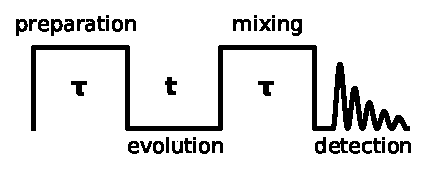
\includegraphics[width=0.5\textwidth]{mq-experiment-schema.pdf}
%   \caption{Схема МК эксперимента ЯМР}
% \end{figure}
\begin{figure}
  \centering
  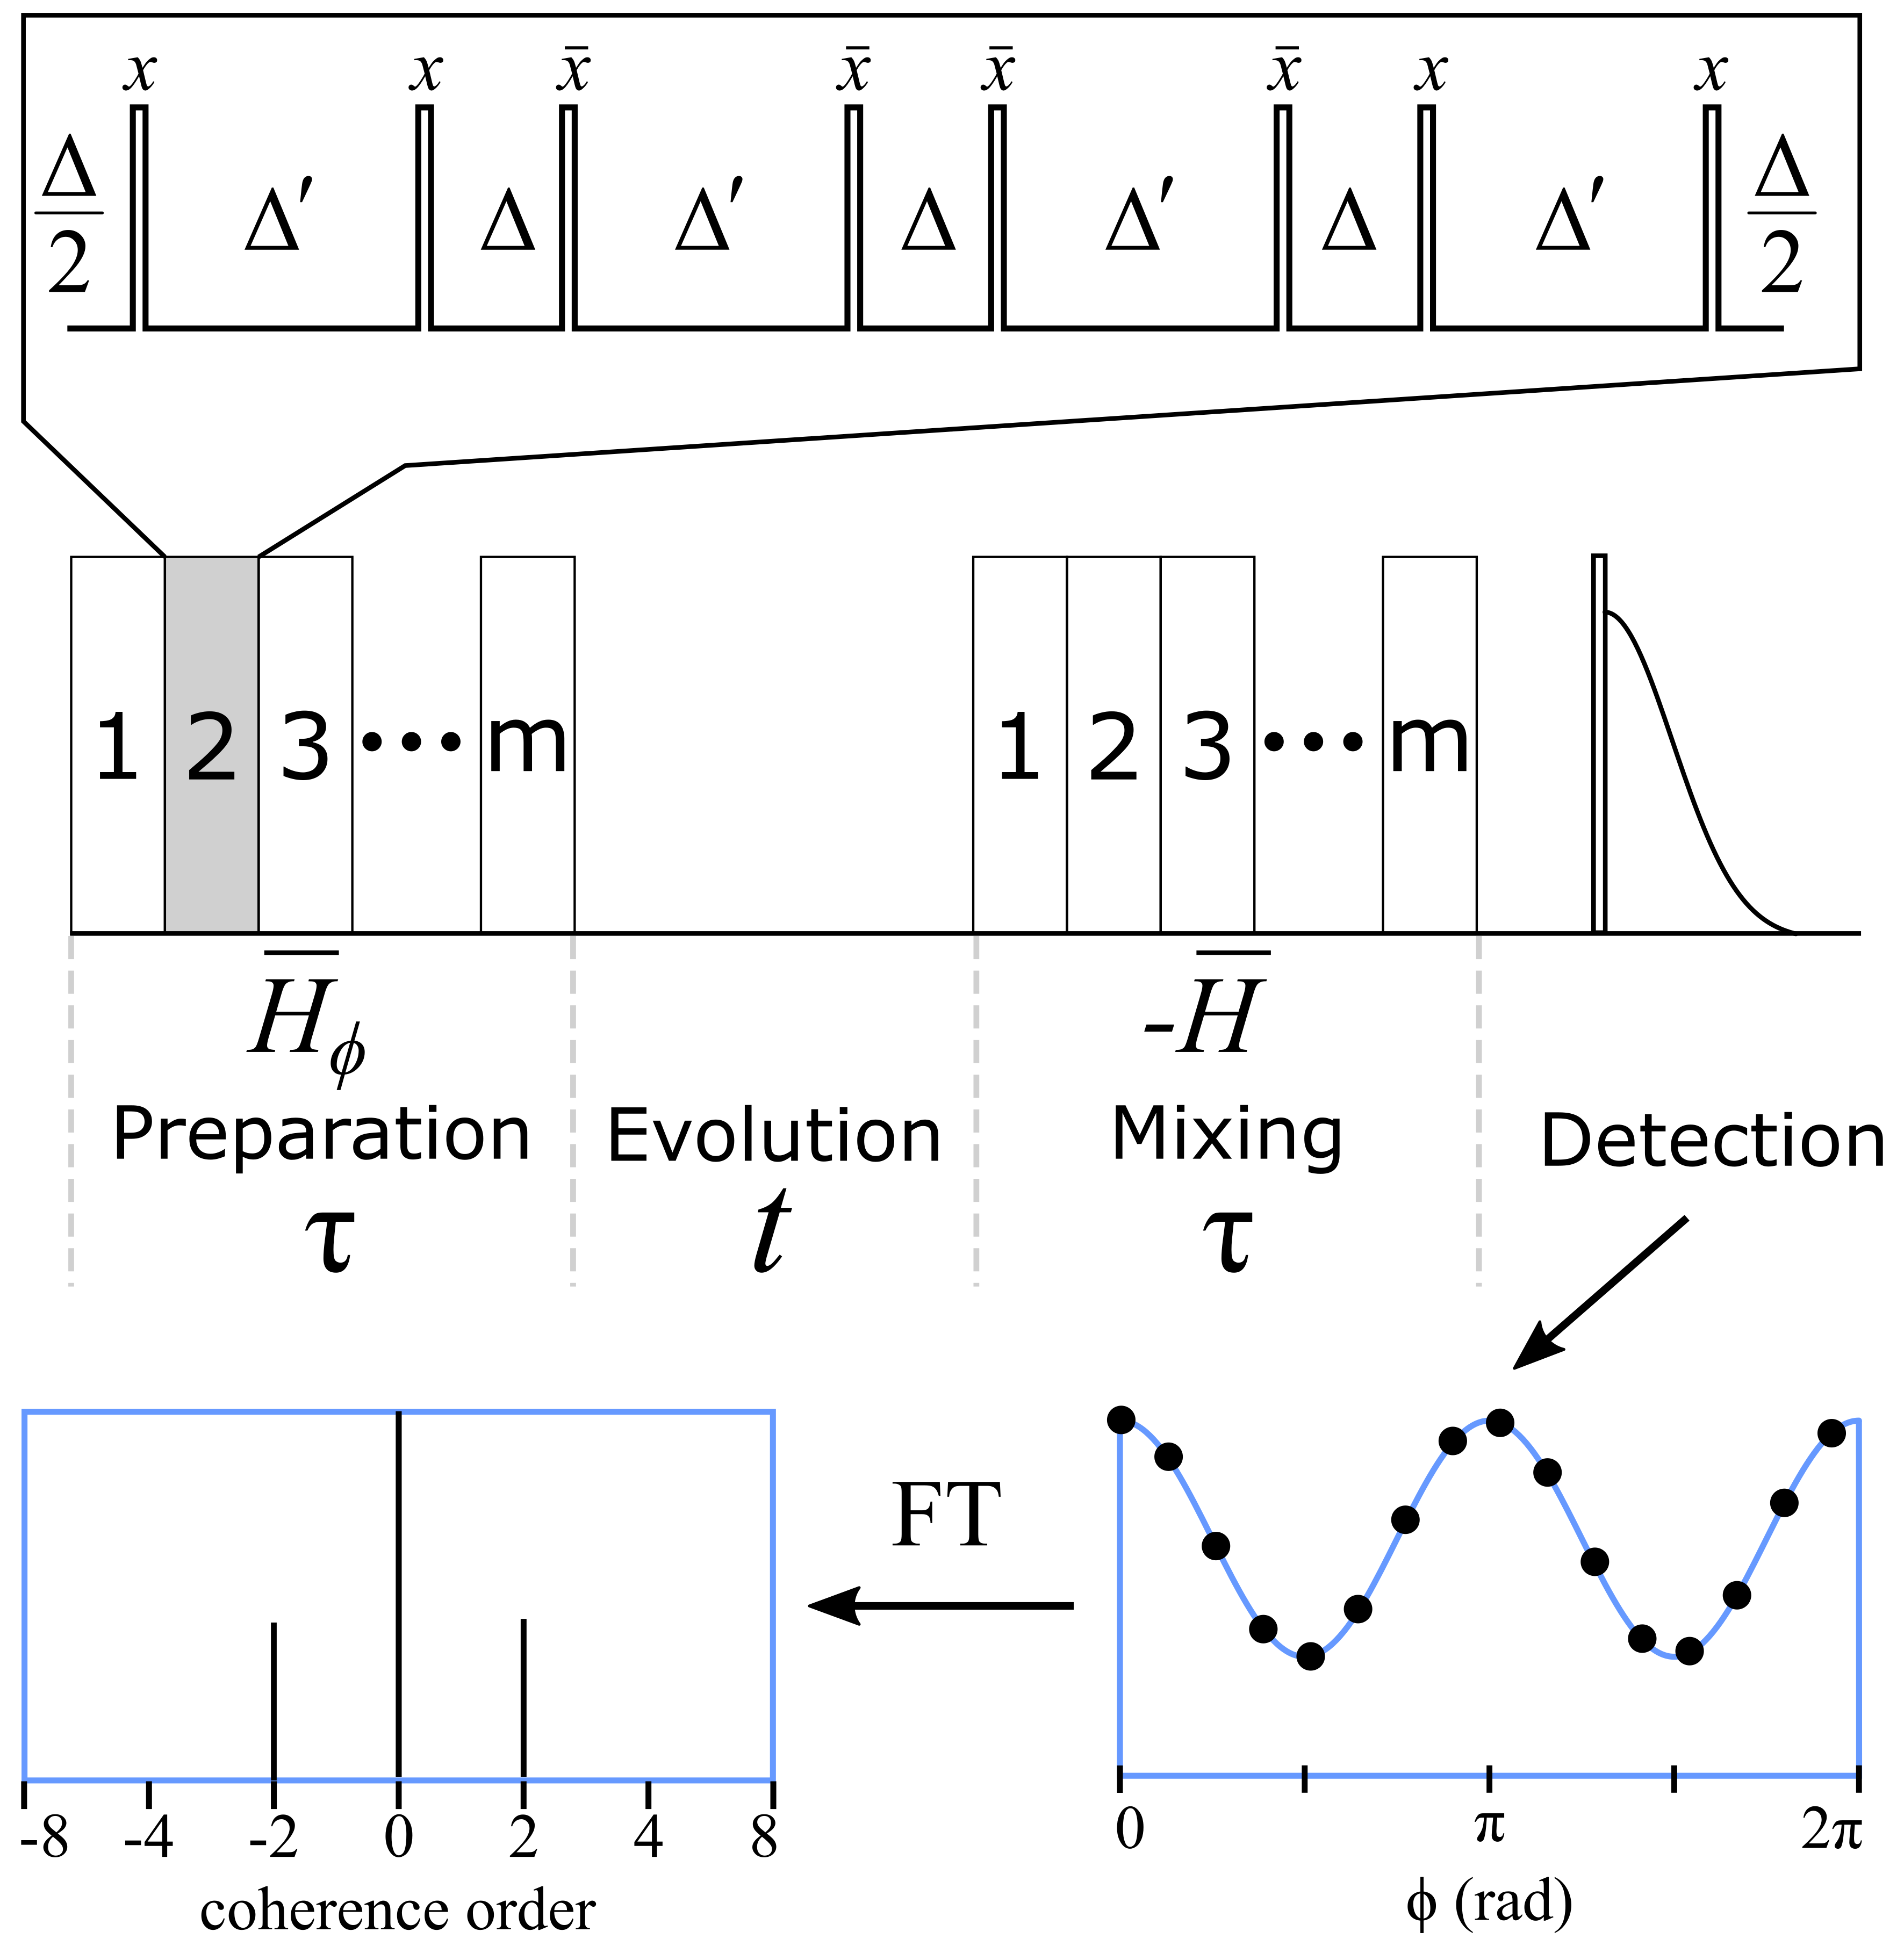
\includegraphics[width=0.5\textwidth]{mq-experiment-pulses-schema.png}
  \caption{Схема МК эксперимента ЯМР}
  \label{fig:mq-experiment-pulses-schema}
\end{figure}

Многоквантовый эксперимент ЯМР состоит из четырех основных периодов (рис.~\ref{fig:mq-experiment-pulses-schema}): подготовительного, свободной эволюции, смешивания и детектирования.
Эти периоды многократно повторяются с инкрементом фазы РЧ-импульсов, облучающих спиновую систему на подготовительном периоде при каждом повторении. Используемая последовательность РЧ-импульсов построена из базовых циклов, состоящих из восьми резонансных $\pi/2$-импульсов (рис. 1).
На подготовительном периоде многоквантового эксперимента ЯМР
система облучается несколькими такими циклами,
что приводит к возникновению многоквантовых когерентностей четного порядка.
При инкременте фазы РЧ-импульсов $\varphi$ несекулярный двухспиновый/двухквантовый гамильтониан (1) принимает следующий вид:
%
\begin{equation}\label{eq:hmq-phased}
    H_\mathrm{MQ}^{\phi} = e^{-2i\phi}H^{(2)} + e^{2i\phi}H^{(-2)}
\end{equation}
%
Использование инкремента фазы РЧ-импульсов позволяет разделить сигналы от многоквантовых когерентностей разных порядков на периоде свободной эволюции [22] (рис.~\ref{fig:mq-experiment-pulses-schema}).

Поскольку многоквантовые когерентности ЯМР не могут наблюдаться непосредственно, они преобразуются в поперечную намагниченность (одноквантовую когерентность) на периоде смешивания. На периоде смешивания спиновая система облучается такой же последовательностью РЧ-импульсов, как и на подготовительном периоде, но фаза импульсов сдвигается на $\pi/2$
(вместо $x$-импульсов подаются  $y$-импульсы).
Формула~(\ref{eq:hmq-phased}) показывает, что при таком сдвиге фазы изменяется знак несекулярного двухспинового/двухквантового гамильтониана (1). Таким образом, на периоде смешивания создаются условия обращения времени [23], необходимые для сфазирования вкладов разных пар спинов в многоквантовые когерентности разных порядков [1].
%
Матрица плотности системы после периода смешивания может быть записана как \cite{Baum1985}
\begin{equation}\label{eq:rho-after-mixing}
  \rho_\mathrm{f}(\tau)
  = e^{i{H_{MQ}}\tau} e^{i\phi I_z} e^{-i{ H_{MQ}}\tau}
  \rho_\mathrm{i}
  e^{i{ H_{MQ}}\tau} e^{-i\phi I_z} e^{-i{H_{MQ}}\tau} ,
\end{equation}
где начальное состояние системы $\rho_\mathrm{i}$
и фаза $\phi$ определяются условиями МК эксперимента ЯМР~\cite{Baum1985}.

Детектирующий импульс подается для переноса намагниченности в плоскость, перпендикулярную внешнему магнитному полю.
Измеряемый сигнал $G_\mathrm{HT}(\tau, \phi)$ определяется выражением
\begin{equation}\label{eq:signal-after-mixing}
  G(\tau, \phi)
  = \tr{\rho_\mathrm{f}(\tau) I_z}
  = \tr{
    e^{iH_{MQ}\tau}e^{i\phi I_z}e^{-iH_{MQ}\tau}
    \rho_\mathrm{i}
    e^{iH_{MQ}\tau}e^{-i\phi I_z}e^{-iH_{MQ}\tau}
    I_z
  }.
\end{equation}
%
Затем записывается одна точка, соответствующая максимальному значению спада свободной индукции на временном интервале $t_2$ для каждого инкремента фазы. Преобразование Фурье относительно инкремента фазы позволяет получать многоквантовые спектры, состоящие из набора узких линий, отвечающих различным порядкам когерентностей [22]. Такой метод существенно сокращает время проведения эксперимента по сравнению с традиционным методом, когда инкремент фазы изменяется пропорционально длительности периода эволюции (метод TPPI [1]).



\subsection{Одномерная цепочка ядерных спинов}
% JMR2019

\begin{figure}[ht]
  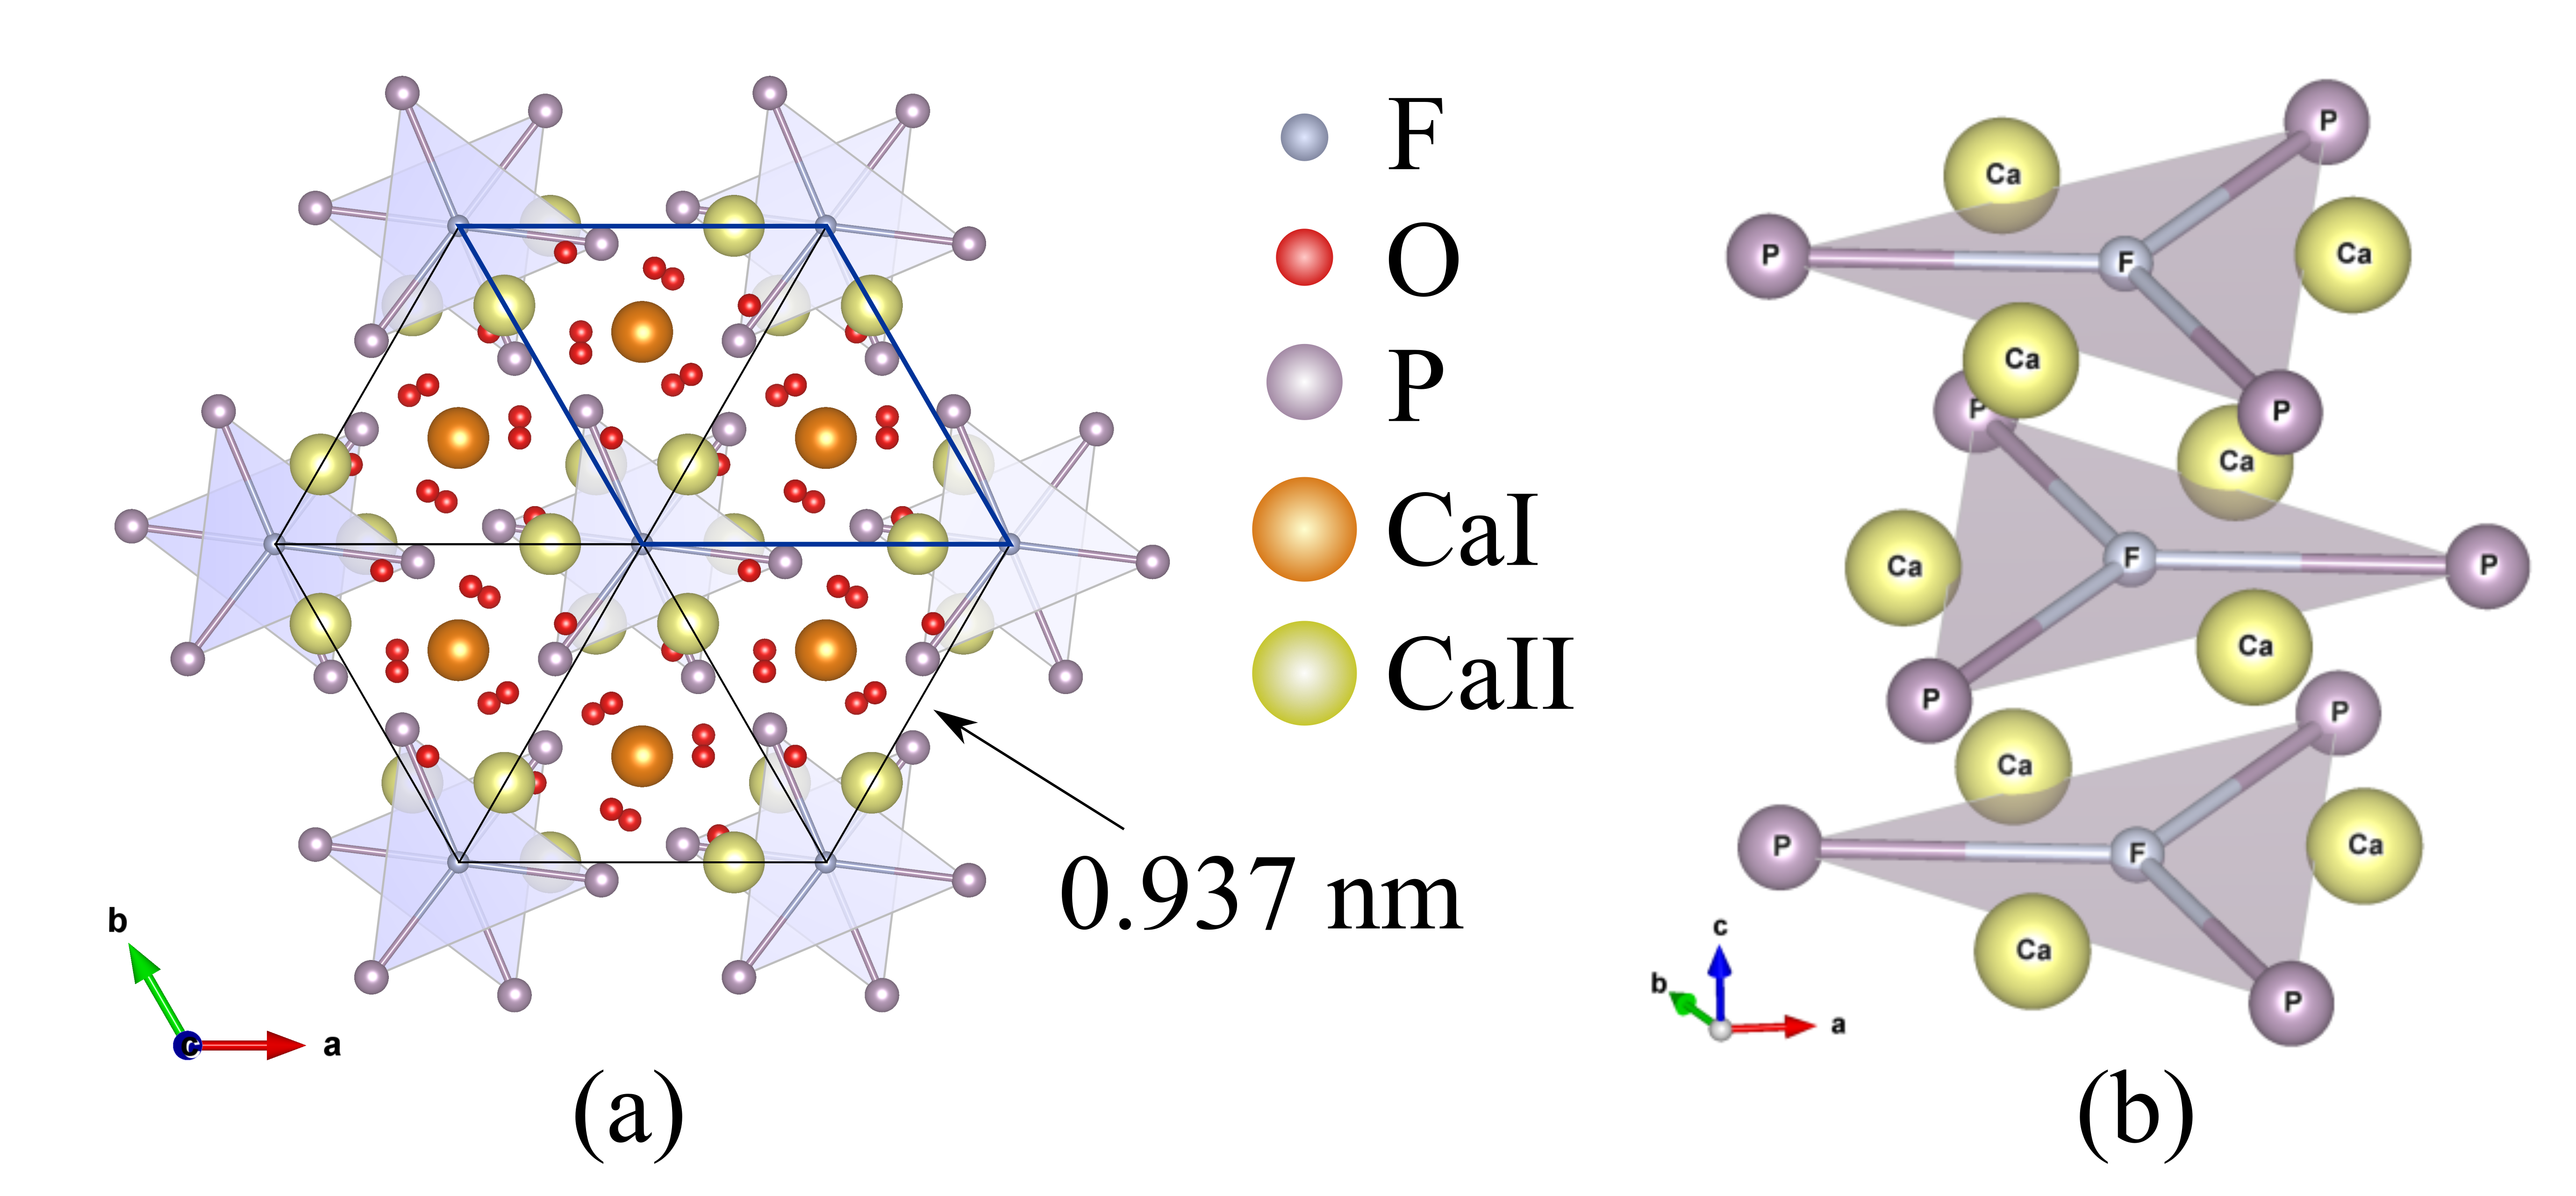
\includegraphics[width=\linewidth]{sample-fap-crystal-structure.png}
  \caption{
    (a) Структура фтористого апатита, $c$-ось направлена перпендикулярно плоскости рисунка.
    Выделена одна ячейка.
    Каждая цепь ядер $^{19}$F, идущая вдоль оси $c$, окружена шестью идентичными цепями на расстоянии $a=9.37$~\r{A}.
    (b) Часть кристаллической структуры FAp, показывающая окружение атомов фтора. Атомы кислорода были удалены для ясности.
    Атомы фтора равномерно разнесены ($r_{FF}=344$~пкм) и расположены в колонны вдоль $c$-оси кристалла.
    Каждый атом фтора окружен тремя равноудаленными атомами фосфора при $r_{FP}=3,67$~\r{A},
    которые расположены в вершинах равносторонних треугольников на плоскости,
    перпендикулярной к $c$-оси, а также тремя ионами CaII на расстоянии 2.34~\r{A}.
  }
  \label{fig:sample-fap-crystal-structure}
\end{figure}
Хотя первый феноменологический подход к многоквантовой динамике ЯМР был развит еще в классической работе [1],
последовательная квантовомеханическая теория в настоящее время развита преимущественно для одномерных систем [11–14].
Теория МК динамики ЯМР в одномерных системах основана на том,
что несекулярный двухспиновый/двухквантовый гамильтониан~(\ref{eq:hmq}),
описывающий многоквантовую динамику,
является $XX$-гамильтонианом,
который для одномерных систем в приближении взаимодействий ближайших соседей может быть точно диагонализован [8].
В результате многоквантовая динамика ЯМР в такой системе может быть исследована аналитически.

% AMR-2020
Одномерные цепочки ядерных спинов являются редкими объектами из-за дальнодействующего характера прямой магнитной дипольной связи.
Такие цепочки принято называть ``квазиодномерными'', поскольку идеальная изоляция спиновых цепочек в природе не встречается.
Cписок квазиодномерных цепочек с прямым магнитным ДДИ,
представленных в литературе,
ограничивается цепочками в кристаллах минералов группы апатита,
такими как 1H и 19F спиновые цепочки в кристаллах гидрокси- и фторапатита [16].
Отличительной особенностью этих структур является то, что расстояние между соседними цепочками примерно в 2,7 раза больше, чем расстояние между ближайшими спинами в цепочке [16]. Ориентируя кристалл так,
чтобы внешнее магнитное поле было направлено параллельно цепочкам,
можно добиться чтобы диполярная связь между ближайшими соседями в одной цепочке была по крайней мере в 40 раз сильнее,
чем со спинами других цепочек.
%
Это позволяет использовать для интерпретации экспериментальных данных модель изолированной спиновой цепочки.
Пeрвые экспериментальные исследования многоквантовой динамики ЯМР одномерных систем были начаты в [16, 17] на монокристалле гидроксиапатита кальция $\mathrm{Ca}_5(\mathrm{PO}_4)_3\mathrm{OH}$ с гексагональной системой гидроксильных протонов.
Другой пример квазиодномерной спиновой цепочки является довольно экзотическим,
поскольку был получен искусственно с помощью изотопной инженерии.
Линейные цепочки изотопов $^{29}$Si были получены в монокристалле кремния, состоящем из бесспинового изотопа $^28$Si~\cite{Itoh2005}.

Структура FAp, изученная с помощью рентгеноструктурного анализа \cite{Elliott1994}, изображена на Рис.~\ref{fig:sample-fap-crystal-structure} (изображения были получены с помощью программного обеспечения VESTA \cite{vesta}).
FAp представляет собой гексагональный кристалл с пространственной группой P63/m
и имеет параметры решетки $a=9.367(1)$~\r{A} и $c=6.884(1)$~\r{A}
(гексагональная ось) с одной формальной единицей Ca$_{10}$(PO$_4$)$_6$F$_2$ на каждую элементарную ячейку.
Таким образом, семь кристаллографически неэквивалентных атомных сайтов в одной ячейке (Рис.~\ref{fig:sample-fap-coherences}a).
Ядра $^{19}$F упорядоченны в линейную цепочку вдоль оси $c$ на гранях элементарных ячеек (Рис.~\ref{fig:sample-fap-coherences}a и b). Эти ядра разделены 1/2 размера решетки (3.44~\r{A}) на позициях z=1/4 и 3/4. При повороте на угол кратный $\pi/3$ углы элементарной ячейки совпадут с шестью ближайшими атомами F$^-$ на расстоянии 9.37~\r{A}   в плоскости перпендикулярной оси $c$. Известно, что в структуре FAp присутствует два изотопа кальция: четыре CaI и шесть CaII. Колонки Ca$^{2+}$ ионов параллельны цепочке ядер F и разделены половиной параметра решетки вдоль $c$-оси. Это 2/5 всех Ca$^{2+}$ ионов в кристалле, и они представлены изотопом CaI. Остальные сайты Ca$^{2+}$, представленные как CaII, расположены в вершинах равносторонних треугольников в плоскости, перпендикулярной $c$-оси. В центрах треугольников располагаются ионы F$^-$. Расстояние межу CaII и ионами F$^-$ 2.34~\r{A}  . Два треугольника повернуты на $60^\circ$ относительно друг друга вокруг $c$-оси. PO$_4^{3-}$ тетраэдры слегка искажены. Это приводит к трем неэквивалентным сайтам кислорода. P можно представить в вершинах равносторонних треугольников, расположенных в шахматном порядке вдоль оси $c$, в плоскости, перпендикулярной оси $c$ в положениях z = 1/4 и 3/4 с ионами F$^-$ в центре (рис.~\ref{fig:sample-fap-coherences}a). Расстояние между F и ближайшими P-ядрами составляет 3.67~\r{A}

% JETP-Lett 2015
В работах [11–14] была разработана теория МК динамики для одномерной цепочки спинов,
связанных диполь-дипольным взаимодействием,
в приближении взаимодействий ближайших соседей.
Было показано,
что в одномерной спиновой цепочке,
первоначально приготовленной в термодинамическом равновесном состоянии,
на подготовительном периоде МК ЯМР эксперимента~\cite{Baum1985},
возникают многоквантовые когерентности только нулевого и плюс/минус второго порядков.
%
Теоретические значения интенсивностей многоквантовых когерентностей ЯМР нулевого $G_0(\tau)$ и плюс/минус второго $G_{\pm2}(\tau)$ порядков
в случае длинных линейных спиновых цепей (с числом спинов $N \gg 1$) определяются формулами
%
\begin{equation}
    \label{eq:coher_g0}
    G_{0}(\tau) = \frac 1 2 + \frac 1 2 J_{0}(4D\tau)
\end{equation}
%
\begin{equation}
    \label{eq:coher_g2}
    G_{\pm2}(\tau) = \frac 1 4 - \frac 1 4 J_{0}(4D\tau),
\end{equation}
где $\tau$ - продолжительность подготовительного периода,
$D = D_{i, i+1}$ – дипольная константа связи ближайших соседей,
а $J_0$ – функция Бесселя первого рода порядка 0.
% Решение верно на относительно небольших временах подготовительного периода.

\begin{figure}[H]
  \centering
  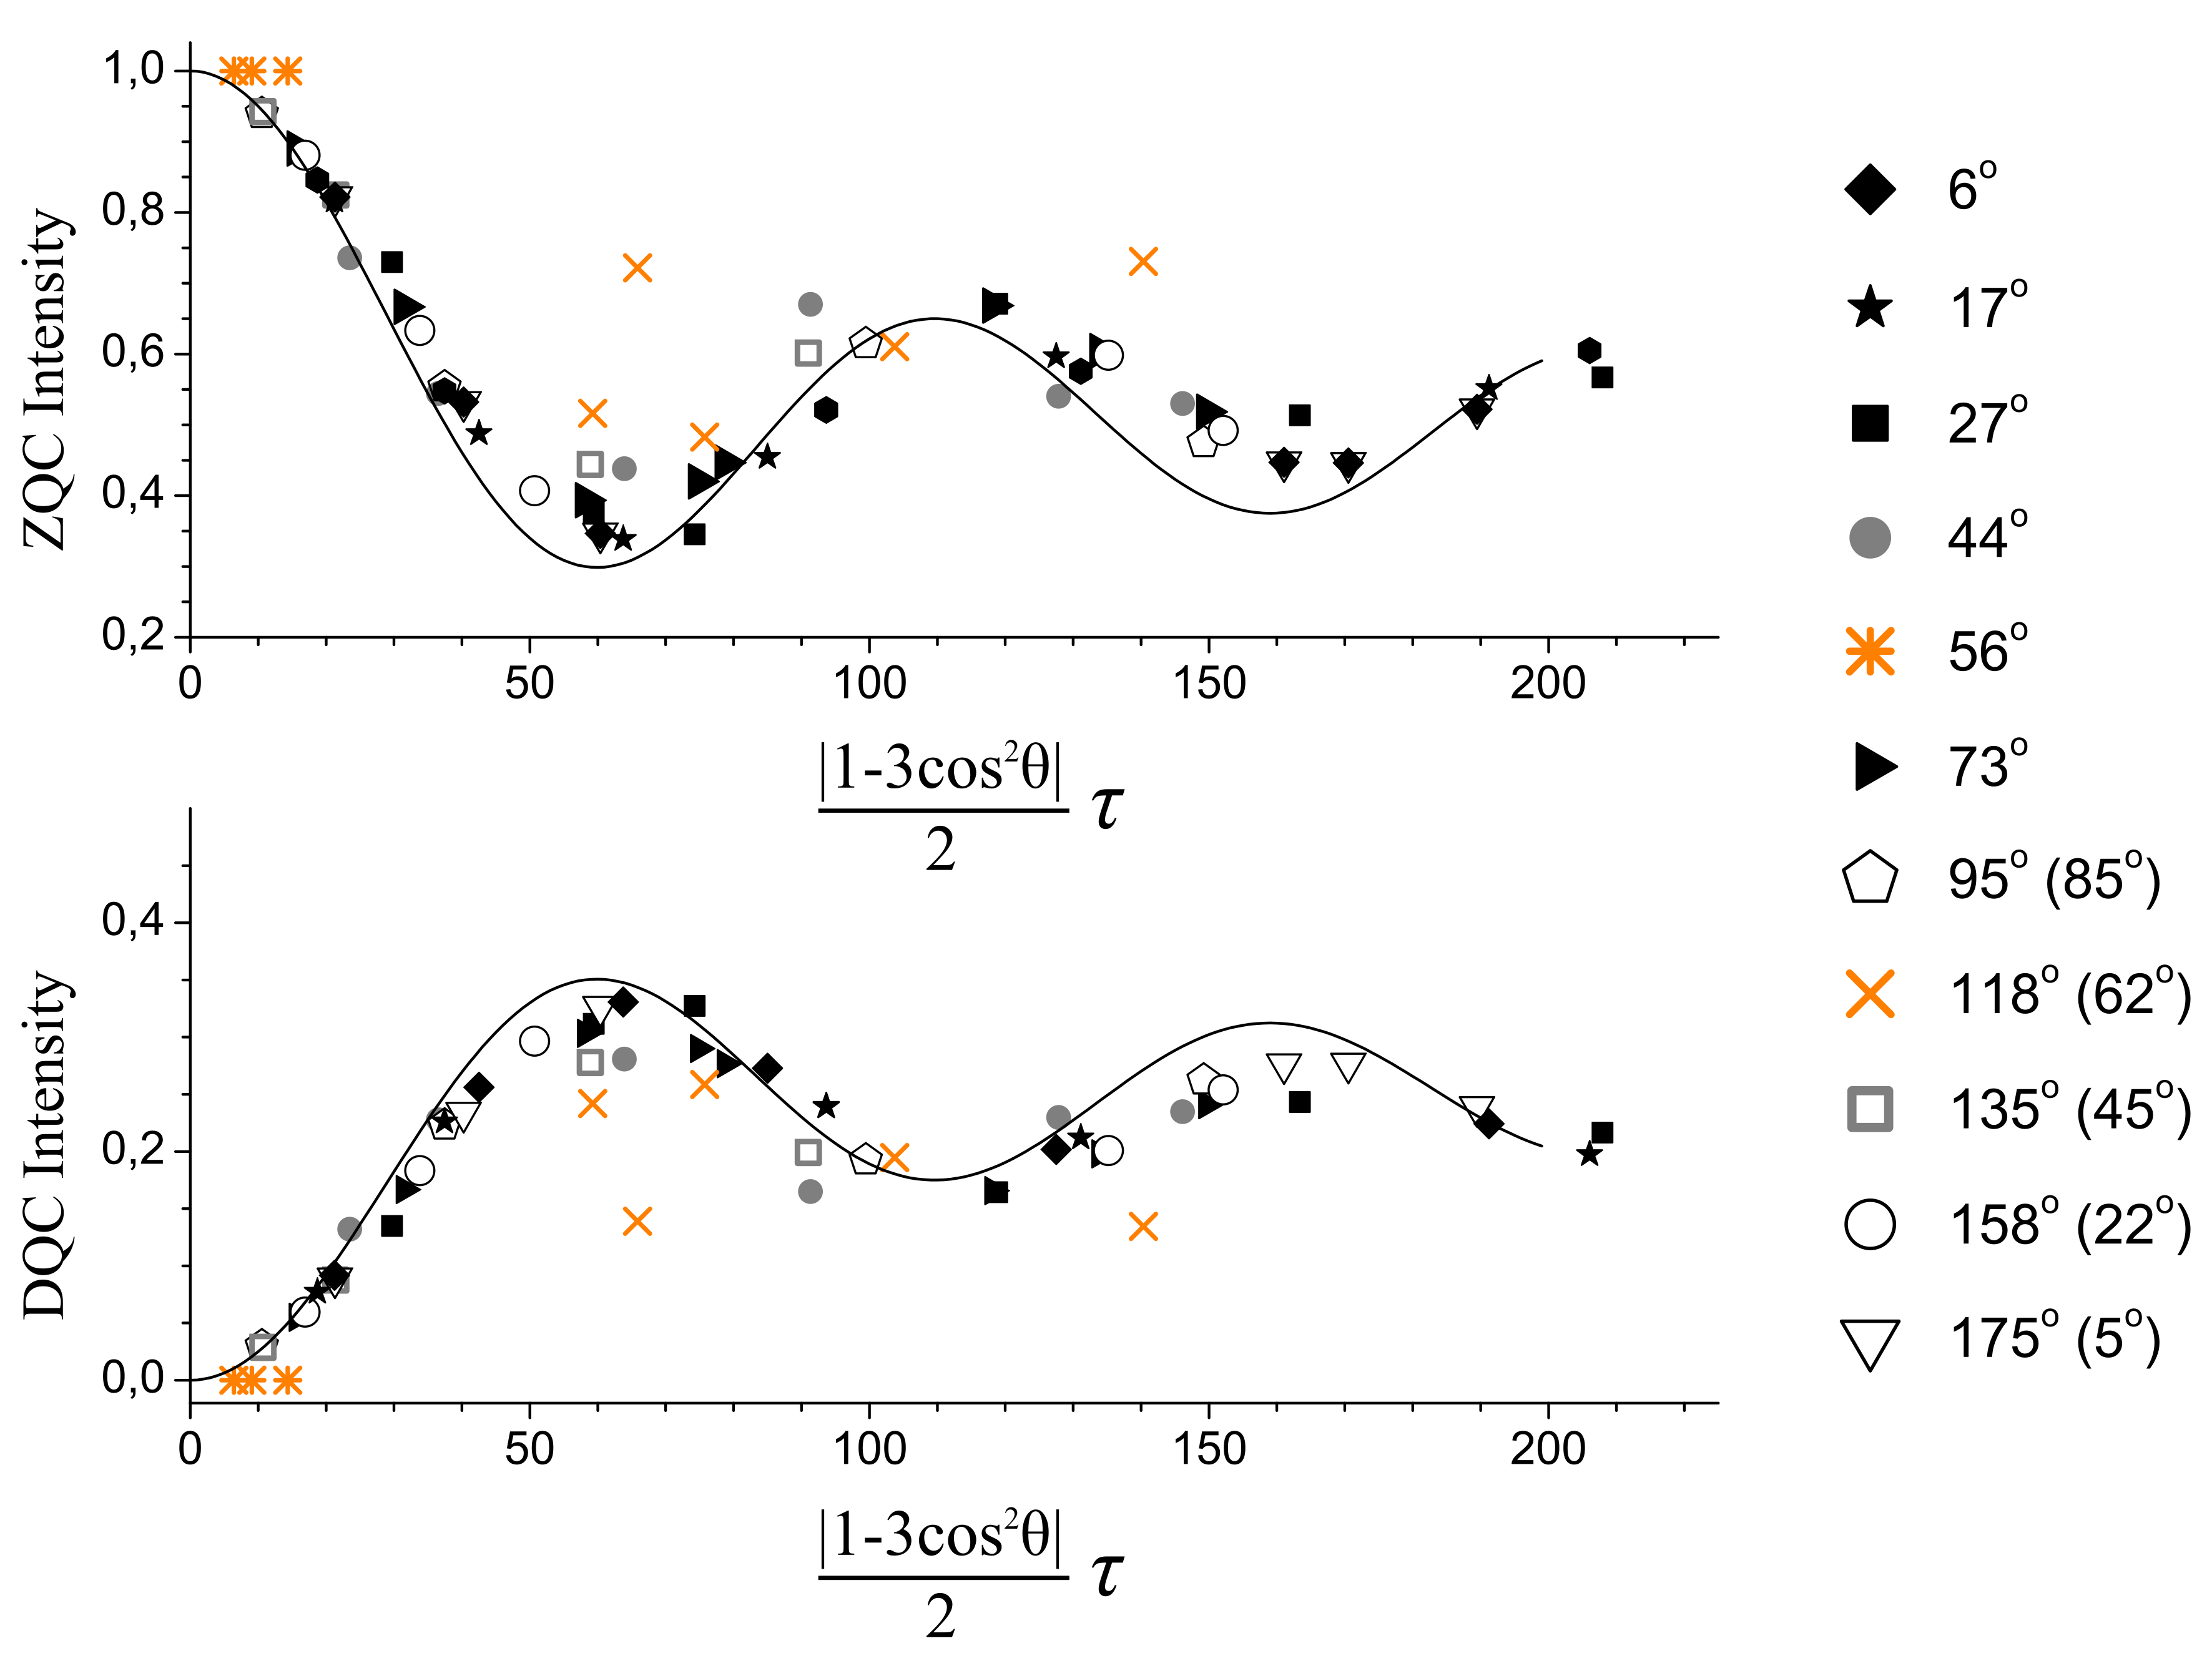
\includegraphics[width=\textwidth]{sample-fap-coherences.png}
  \caption{
    Зависимости интенсивностей МК ЯМР когерентностей нулевого $G_0(\tau)$ (сверху) и плюс/минус второго $G_{\pm2}(\tau)$ (снизу) порядков
    от масштабируемой длительности~$\bar\tau$ подготовительного периода для различных ориентаций образцов.
    Экспериментальные значения показаны в виде точек,
    a соответствующие теоретические (Ур.~(\ref{eq:coher_g0})~и~(\ref{eq:coher_g2})) результаты показаны сплошными линиями.
  }
  \label{fig:sample-fap-coherences}
\end{figure}

Принимая во внимание, что единственный аргумент, влияющий на эволюцию МК когерентности в уравнениях~(\ref{eq:coher_g0})~(\ref{eq:coher_g2}) равен $4D\tau$,
зависимость интенсивностей МК когерентности от периода подготовки для различной ориентации спиновой цепи можно обобщить простым способом\cite{Bochkin2019jmr},
введя безразмерный масштабный коэффициент $|D(\theta)/D (0)|$ для длительности подготовительного периода $\tau$.
Другими словами, можно ввести масштабированную ось длительности подготовительного периода:
%
\begin{equation}\label{eq:scaled-tau}
 \bar\tau = \left| \dfrac{1 - 3\cos^2{\theta}}{2} \tau \right|,
\end{equation}
%
для которой интенсивности МК когерентностей нулевого и плюс/минус второго порядков,
полученные при различных ориентациях,
коллапсируют на единую заданную кривую $G_0(\tau)$ и $G_{\pm 2}(\tau)$ соответственно (Рис.~\ref{fig:sample-fap-coherences}).
Абсолютное значение в выражении~(\ref{eq:scaled-tau}) объясняется тем фактом,
что интенсивности МК когерентности нечувствительны к знаку константы дипольной связи,
согласно уравнениям~(\ref{eq:coher_g0})~и~(\ref{eq:coher_g2}).

Экспериментально наблюдаемые интенсивности МК когерентностей ЯМР достаточно хорошо следуют теоретическим предсказаниям
в рассматриваемом диапазоне длительностей подготовительного периода.
Очевидные отклонения на Рис.~\ref{fig:sample-fap-coherences}) наблюдаются только для ориентаций,
близких к магическим углам ($56^\circ$ и $118^\circ$,
где дипольная связь между спинами в одной цепи становится слабой.
Для ориентации $56^\circ$ появление когерентностей порядка $\pm2$ не наблюдается.
МК когерентности  ЯМР для ориентации $118^\circ$,
по-видимому, обусловлены взаимодействиями спинов в разных цепях и, следовательно, не следуют общей тенденции.
Некоторые небольшие отклонения наблюдаются для углов $44^\circ$ и $135^\circ$,
которые все еще близки к магическому углу.
Последние отклонения можно отнести к большему влиянию погрешности установки угла.
Изменения дипольной константы в этом диапазоне являются самыми сильными,
что приводит к большей ошибке в определении поправочного коэффициента для времени подготовки.
Ориентации цепи, близкие к перпендикулярному внешнему магнитному полю,
не показывают существенных отклонений МК интенсивностей несмотря на то,
что внутрицепочечное дипольное взаимодействие уменьшается примерно в два раза,
а константа межцепочечного взаимодействия максимальна.
Учитывая, что единственным регулируемым параметром в теории является дипольная константа связи,
между ближайшими соседями в цепи, данные очень хорошо соответствуют кривой.


% mrjs-2019
% JETP-2018

% \begin{figure}
%   \centering
%     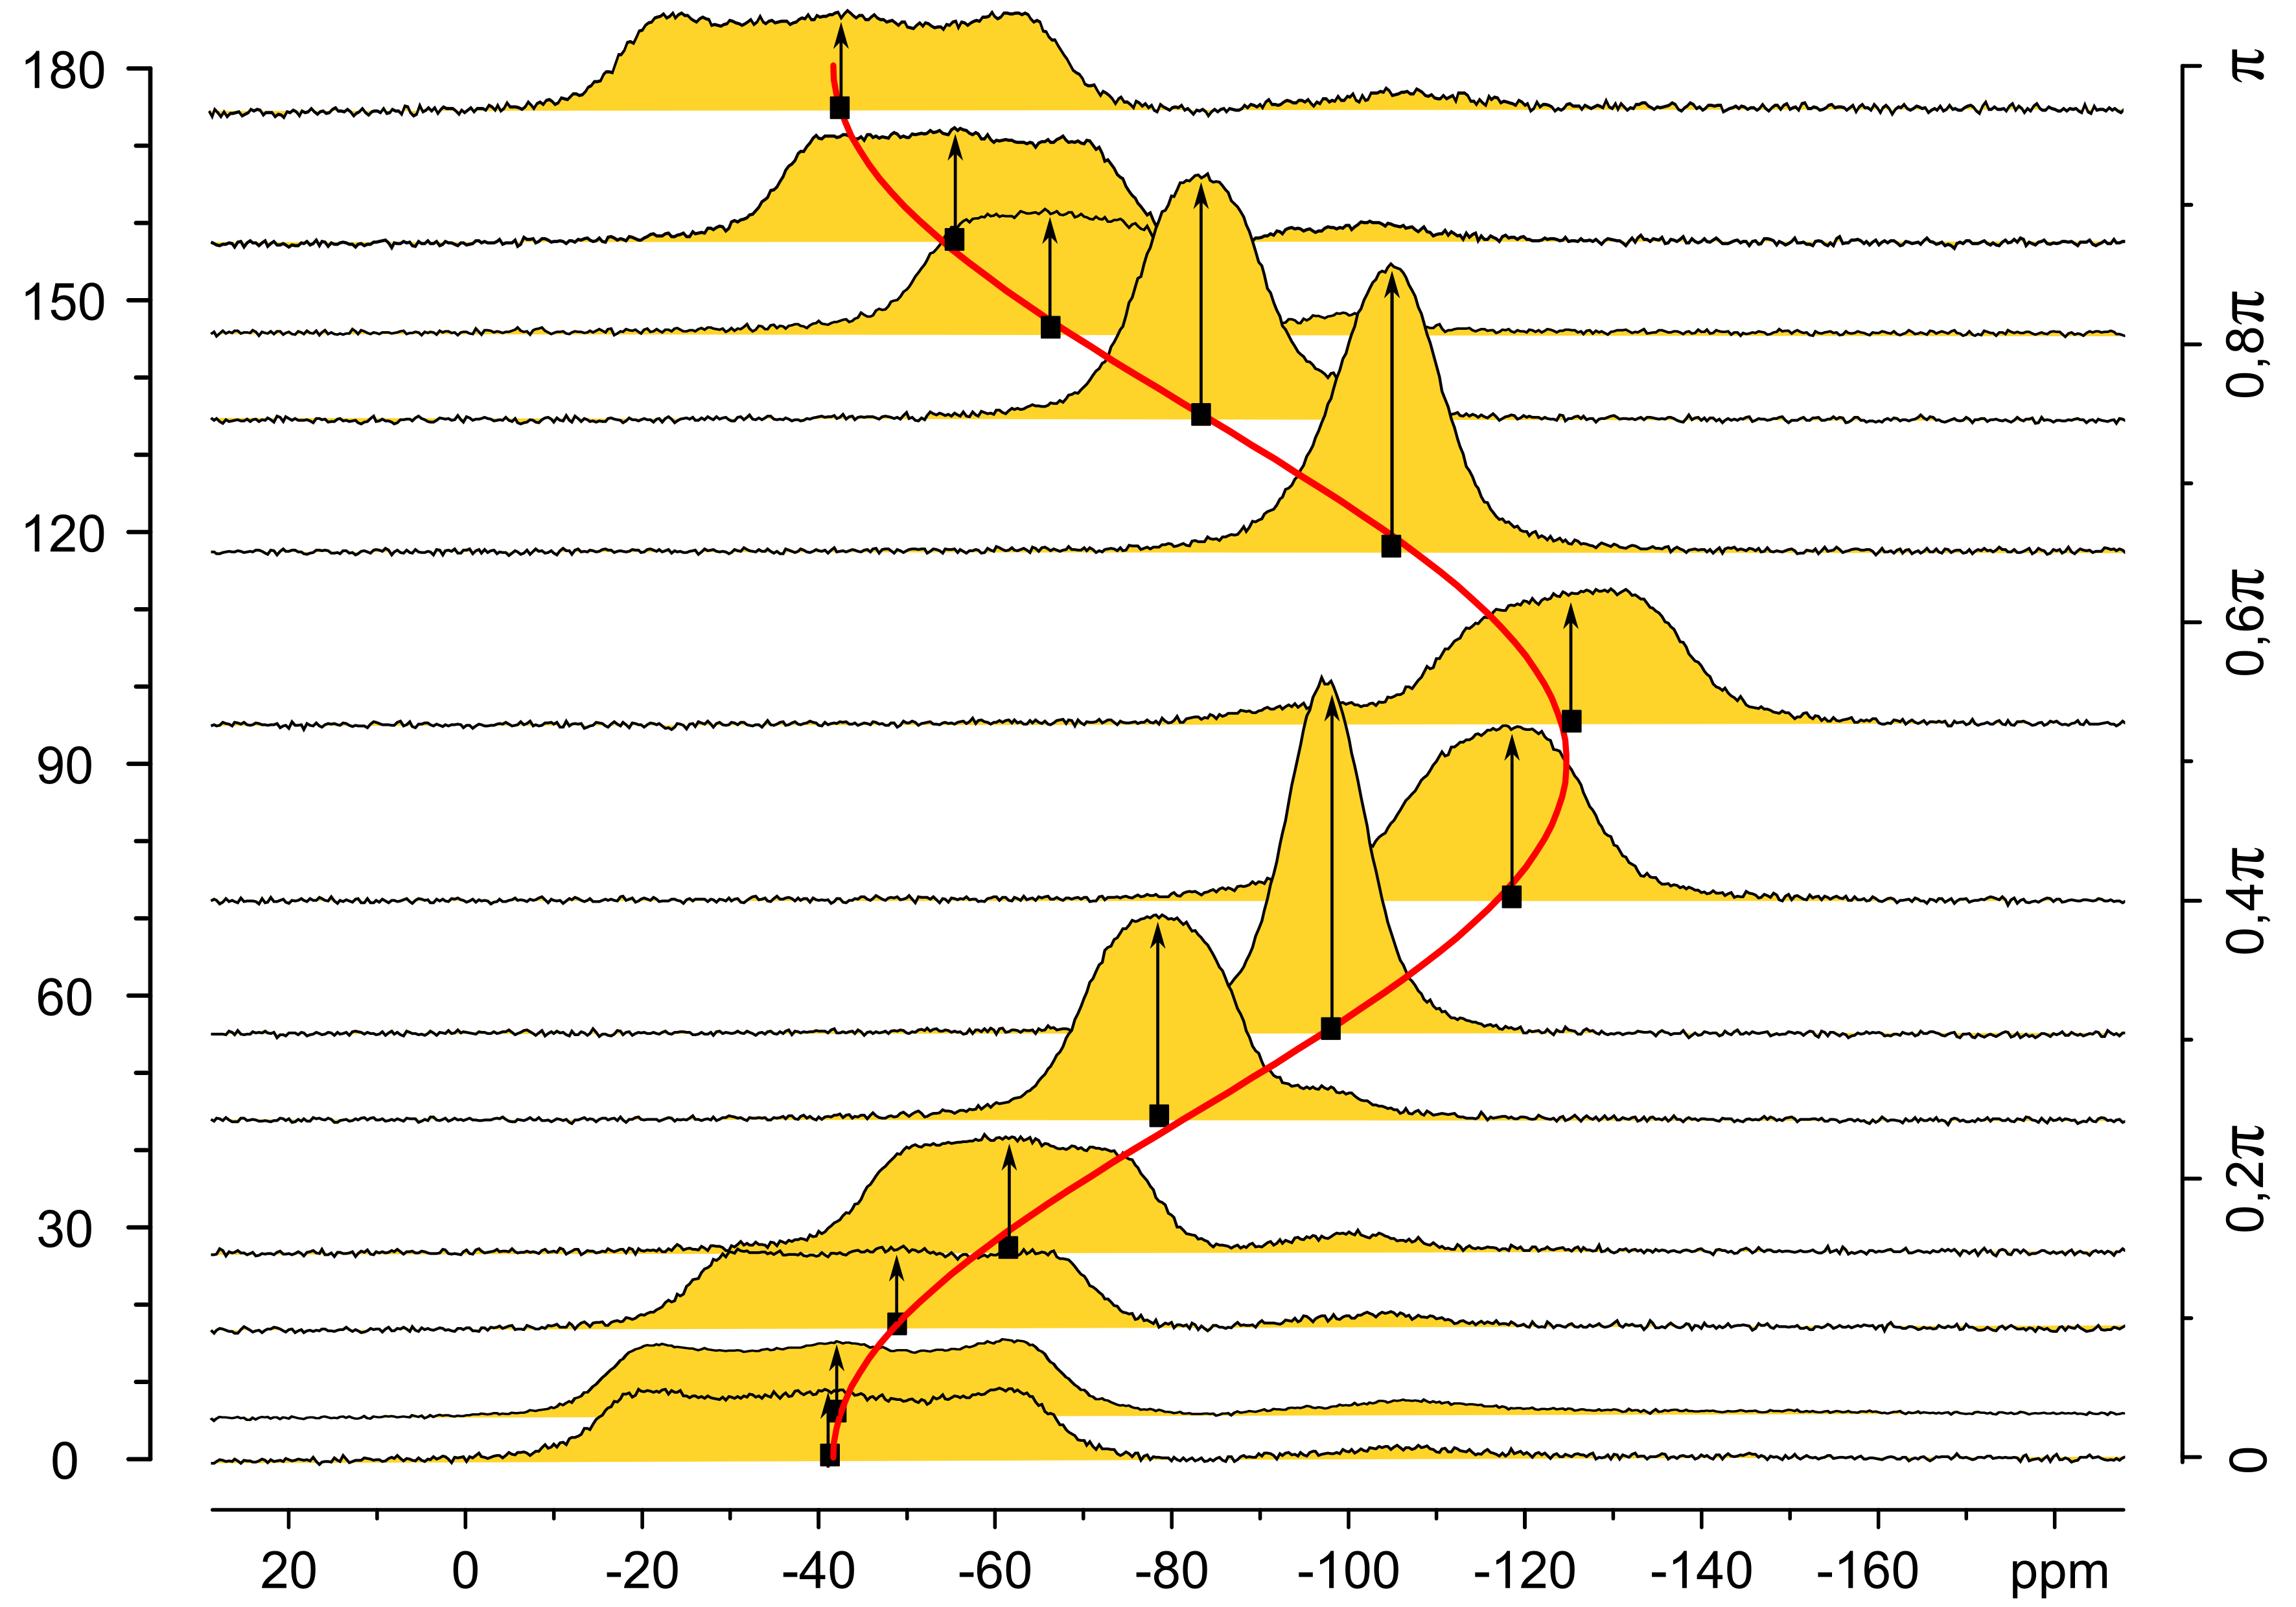
\includegraphics{sample-fap-nmr-spectrum.png}
%     \caption{Изменение $^19$F ЯМР спектра фтористого апатита во время вращения $c$-оси кристалла вокруг оси перпендикулярной направлению внешнему магнитного поля}
%   \label{fig:my_label}
% \end{figure}

\subsection{Зигзагобразная цепочка ядерных спинов}
% JMR-2020 G.A. Bochkin and et al., \textit{J. Magn. Res.} \textbf{319}, 106816, (2020)
% AMR-2020

\begin{figure}
  \centering
  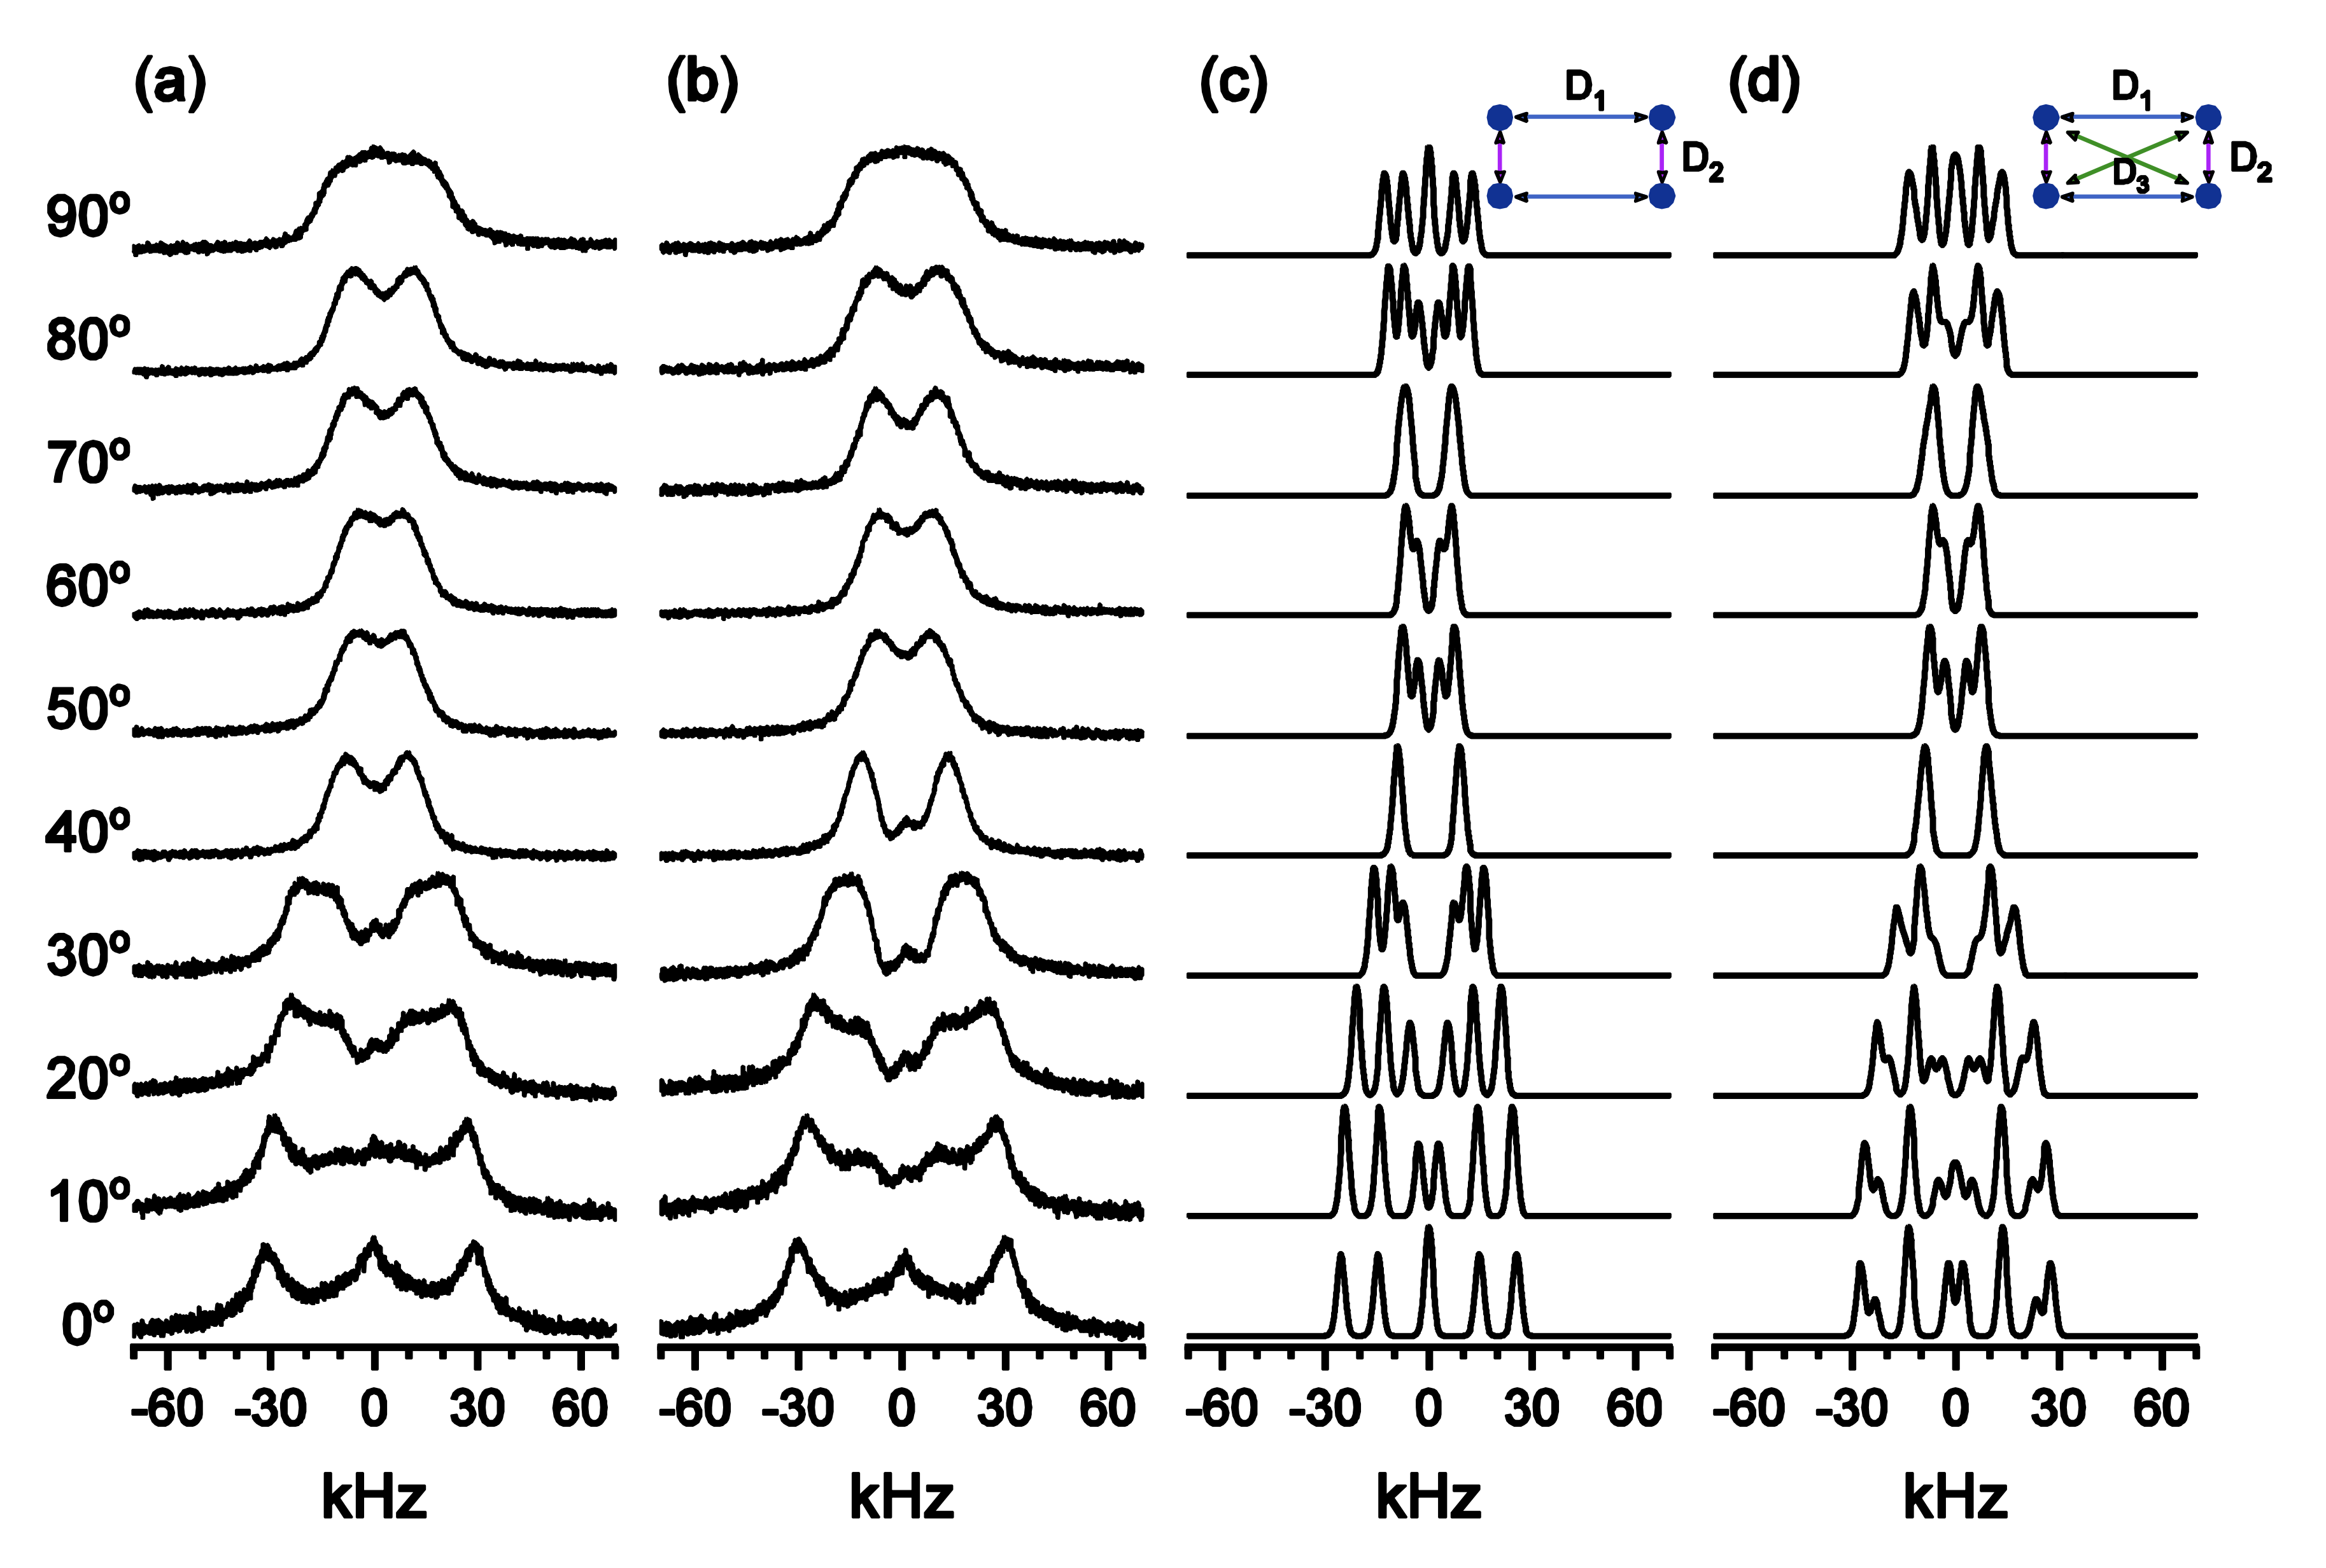
\includegraphics[width=\textwidth]{sample-hambergite-nmr-spectrum.png}
  \caption{
    Спектры ЯМР протонов $^1$H монокристалла гамбергита при вращении в двух различных плоскостях.
    Ось ординат --- это угол между осью цепи ($c$-ось кристалла) и внешним магнитным полем.
    Экспериментальные данные в случае, когда
    ось вращения перпендикулярна $c$-оси и параллельна плоской плоскости кристалла,
    и когда перпендикулярна $c$-оси и плоской плоскости,
    изображены на (a) и (b) соответственно.
    Теоретические спектры для модельной цепочки,
    состоящей из четырех спинов, соединенных в кольцо (прямоугольник),
    с учетом только ближайших соседей и включая соседние взаимодействия,
    изображены на (c) и (d) соответственно.
  }
  \label{fig:sample-hambergite-nmr-spectrum}
\end{figure}

\begin{figure}
  \centering
  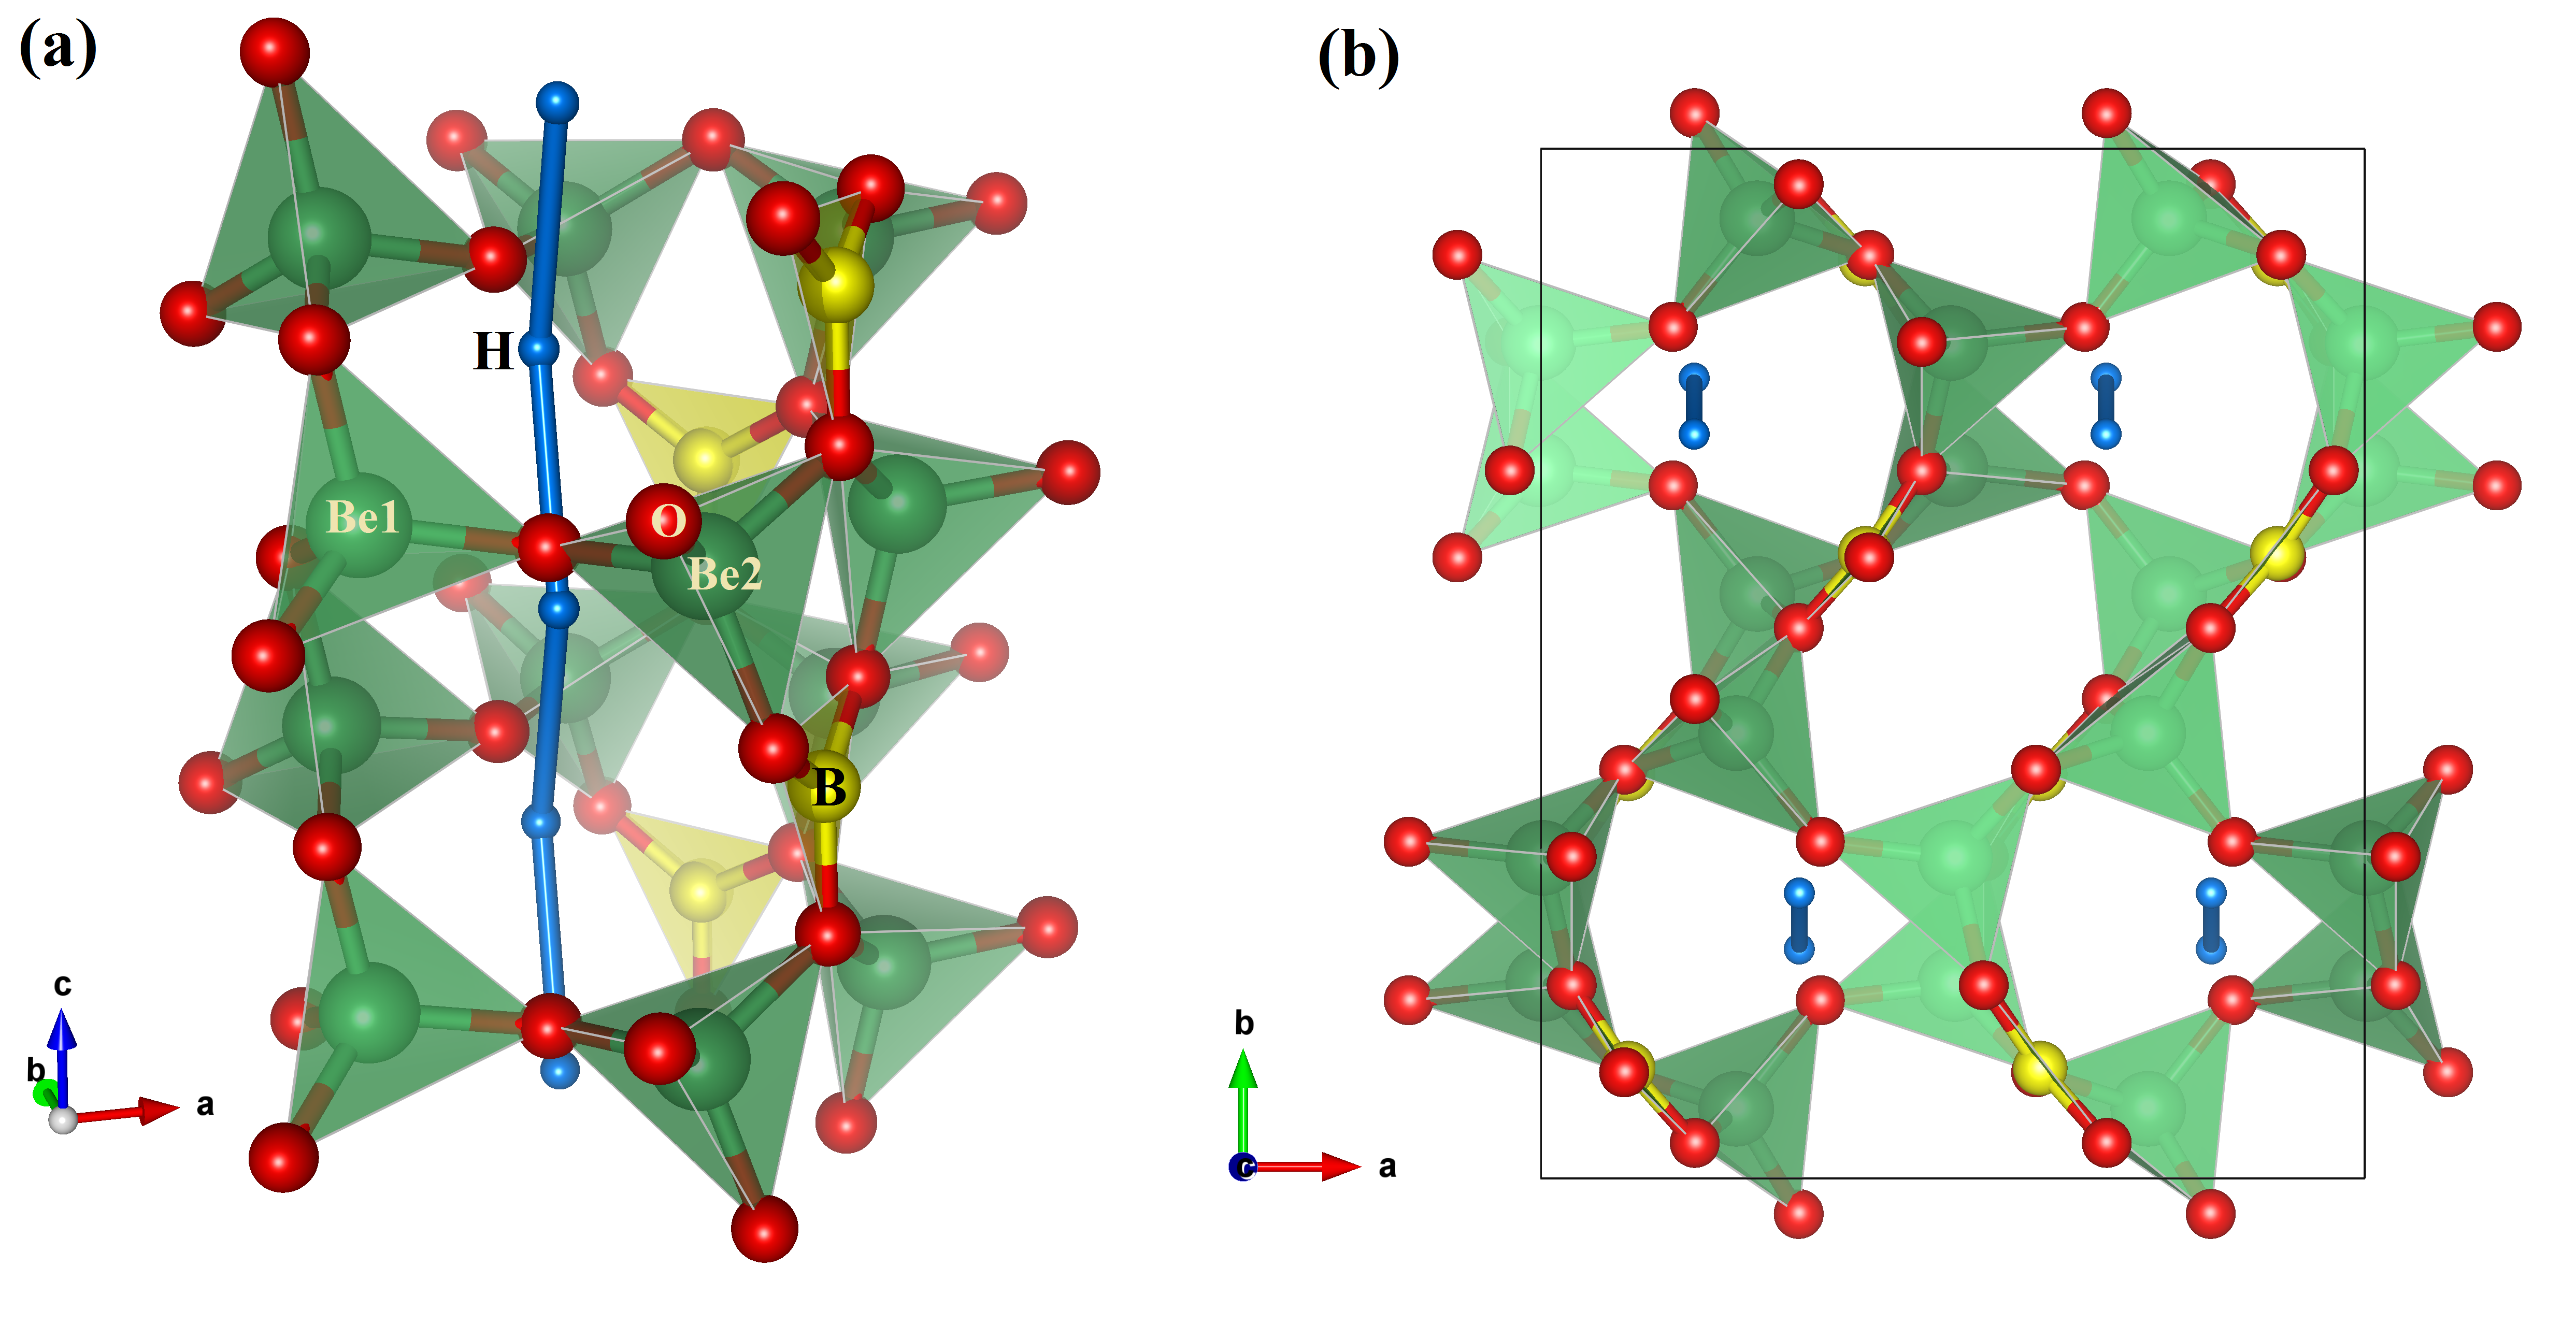
\includegraphics[width=\textwidth]{sample-hambergite-structure.png}
  \caption{
    The structure of hambergite Be2BO3(OH). a One proton chain and neighboring atoms. b The view along the crystallographic c axis
    Структура гамбергита $\mathrm{Be}_2\mathrm{BO}_3(\mathrm{OH})$.
    (a) Цепочка протонов и соседние атомы.
    (b) Вид вдоль кристаллографической $c$-оси.
  }
  \label{fig:sample-hambergite-structure}
\end{figure}
% AMR-2020
В этом разделе будет рассмотрена экзотическая модель спиновой цепочки с чередующейся дипольной связью.
До сих пор данная структура не была исследована в МК эксперименте ЯМР.
Примером такой спиновой модели является квазиодномерная цепочка гидроксильных протонов в кристаллах гамбергита $\mathrm{Be}_2\mathrm{BO}_3(\mathrm{OH})$ [15, 17].
Химический состав и кристаллическая структура гамбергита существенно отличаются от структуры апатита.
На первый взгляд, эти различия не в пользу гамбергита,
если рассматривать его как спиновую цепочку.
Относительная плотность ядер, составляющих цепочку (ядра $^1$Н),
в гамбергите значительно больше, чем в апатите (ядра $^{19}$F или $^1$Н).
Вследствие изолируемость отдельных спиновых цепочек хуже.
Количество других ядер,
обладающих значительным магнитным   моментом,
в гамбергите также больше.
Тем не менее гамбергит демонстрирует тонкую структуру спектров ЯМР $^1$Н (Рис.~\ref{fig:sample-hambergite-nmr-spectrum}),
характерную для одномерных цепочек.
Расчеты второго момента $^1$Н Ван Влека в работе~\cite{Bochkin2020jmr} показывают,
что основной вклад вносят спины в одной цепи,
что сравнимо со случаем апатита.
Особенностью $^1$Н спиновых цепочек гамбергита является то,
что спины в них расположены не вдоль прямой линии,
как в случае апатита,
а образуют зигзаг вдоль направления цепочки (Рис.~\ref{fig:sample-hambergite-structure}).
Таким образом, в зависимости от ориентации во внешнем магнитном поле,
цепочка может рассматриваться как однородная,
с равными дипольными константами среди всех пар ближайших спинов,
или зигзагообразная,
где дипольная связь между ближайшими соседями чередуется между двумя значениями для последовательных пар спинов.
Главным преимуществом зигзагобразной цепочки является то факт,
что в МК эксперименте ЯМР возникают когерентности плюс/минус четвертого порядка,
в отличии однородной цепочки, в которой возникают когерентности только нулевого и плюс/минус второго порядков.

Гамбергит представляет собой орторомбический кристалл с пространственной группой Pbca
и параметрами решетки a = 9,762(2)~\r{A}, b = 12,201(2)~\r{A} и c = 4,430(1)~\r{A} [24].
Число структурных единиц в элементарной ячейке равно Z = 8.
Кристаллическая структура гамбергита показана на Рис.~\ref{fig:sample-hambergite-structure}.
Структура кристалла гамбергита может быть описана [22-25] как состоящая из двух различных строительных блоков:
$\mathrm{BeO}_3(\mathrm{OH})$ тетраэдров
и $\mathrm{BO}_3$ треугольников.
Имеются две различные позиции Be,
каждая из которых координируется тремя атомами O и группой OH.
Каждый негидроксильный атом кислорода в тетраэдрах $\mathrm{BeO}_3(\mathrm{OH})$
разделяется с другой единицей $\mathrm{BeO}_3(\mathrm{OH})$
и треугольником $\mathrm{BO}_3$.
Боратная группа существует в виде почти идеального кислородного треугольника с атомом бора в центре.
Группа OH разделяется между двумя тетраэдрами $\mathrm{BeO}_3(\mathrm{OH})$,
а треугольники $\mathrm{BO}_3$ лежат в плоскости, параллельной оси $c$.
Такое межполиэдрическое соединение приводит к каркасоподобной структуре с искаженными каналами,
идущими вдоль $c$-оси.
Один из двух видов каналов содержит зигзагообразные цепочки спинов $^1$H.
Эти цепочки лежат в плоскостях, параллельных $bc$-плоскости.

\begin{table}[h]
  \centering
  \begin{tabular}{|c|c|c|c|}
    \hline
    Изотоп & Природное содержание, \% & Гиромагнитное отношение, $\frac{\mbox{рад}}{c \cdot T}$ & Спин \\ %  рад с$^{-1}$ Т$^{-1}$
    \hline\hline
    $^9$Be & 100 & $3,75966 \times 10^7$ & 3/2 \\
    \hline
    $^{10}$B & 19,9 & $2.87468 \times 10^7$ & 3 \\
    \hline
    $^{11}$B & 81,1 & $8.584707 \times 10^7$ & 3/2 \\
    \hline
  \end{tabular}
  \caption{
    ЯМР-активным ядра в структуре гамбергита.
   }
  \label{tab:hambergite-isotopes}
\end{table}

Оценим применимость модели одномерных спиновых цепочек для кристалла гамбергита,
на основе атомных координат, предоставленных Гатта и др. [24].
Провем сравнение со структурой фторапатита,
который, как известно,
является хорошей моделью одномерной цепи в широком диапазоне ориентаций во внешнем магнитном поле [26].
Ячейки фторапатита и гамбергита сравнимы по размеру (объемы $526.0$~\r{A}$^3$ и $527.6$~\r{A}$^3$, соответственно),
но последний содержит в 4 раза больше протонов
(каждая ячейка содержит 8 протонов, принадлежащих 4 цепочкам).
Расстояние между ближайшими протонами в гамбергите составляет $2.312$~\r{A}.
Угол между ближайшими соседями и направлением цепи постоянен и составляет приблизительно $16.7^\circ$.
Расстояние до ближайшего протона в соседней цепи составляет $4.940$~\r{A}.
Из этого следует, что изоляция спиновых цепей в гамбергите должна быть намного хуже, чем во фторапатите.
Действительно, ближайшие спины соседних цепочек в гамбергите находятся только в $2.1$ раза дальше,
чем ближайшие спины в цепочке,
по сравнению с почти 3 разами во фторапатите.
Расстояние между ближайшими протонами в гамбергите постоянно,
но они не лежат вдоль одного направления,
в отличие от фторапатита,
где спины одинаково расположены вдоль $c$-оси.
Спины в гамбергите расположены цепочками вдоль $c$-оси зигзагообразно.
Плоскости цепочек параллельны $bc$-плоскости  (см. Рис.~\ref{fig:sample-hambergite-structure}).
Ближайшие соседи в цепочке лежат строго вдоль $c$-оси кристалла
и расстояние между ними равно параметру латентности $c = 4.43$~\r{A}.
Расстояние между плоскостями цепочки вдоль направления $a$ равно половине этого параметра $a/2 = 4.881$~\r{A}.
Расстояние между осями цепей вдоль направления $b$ приблизительно равно половине этого параметра $b/2 = 6.101$~\r{A}.
Аналогично случаю расположения спинов вдоль $c$-оси,
оси цепей вдоль направления $b$ расположены в шахматном порядке (см. Рис.~\ref{fig:sample-hambergite-structure}b и Рис.~\ref{fig:sample-hambergite-structure}c).
В орторомбической системе гамбергита две ближайшие цепи лежат в направлении $a$.
Взаимодействие с двумя ближайшими протонами в этих цепях в 17 раз меньше,
чем взаимодействие ближайших спинов в цепи.
Взаимодействие с остальными окружающими спинами по крайней мере в 30 раз слабее.
Другим важным моментом, который необходимо учитывать в структуре гамбергита,
являются гетероядерные диполярные взаимодействия,
поскольку число магнитно-активных изотопов больше по сравнению с фторапатитом.
Ядра кислорода можно смело игнорировать из-за низкой природной распространенности и низкого гиромагнитного отношения,
но остальные ядра в структуре гамбергита являются ЯМР-активными (см. Таблицу~\ref{tab:hambergite-isotopes}).
Тем не менее расчеты~\cite{Bochkin2020jmr},
учитывающие реальную геометрию и разницу в магнитных моментах,
показывают, что доминирует дипольная связь между спинами в одной цепи.
Вклад, обусловленный дипольным взаимодействием со спинами в одной цепочке, составляет более 96\% от общего второго момента,
когда цепочка ориентирована вдоль внешнего магнитного поля.
Этот вклад уменьшается до 88\% для 1H спиновых цепочек гамбергита,
наклоненных на 30 градусов от внешнего магнитного поля.
Экспериментальная форма линии ЯМР $^1$H может быть описана
с учетом взаимодействия c относительно небольшим количеством ближайших спинов в цепочке.
Полученные результаты подтверждают,
что спины $^1$H в кристаллах гамбергита могут служить хорошей моделью квазиодномерной спиновой цепи.


\subsection{Модель эквивалентных спинов}
\label{sec:model-equivalent-spins}
% J. Baugh, A. Kleinhammes, D. Han, Q. Wang, and Y. Wu, Science 294, 1505 (2001).
\begin{figure}[H]
  % \begin{subfigure}[t]{0.32\textwidth}
  %   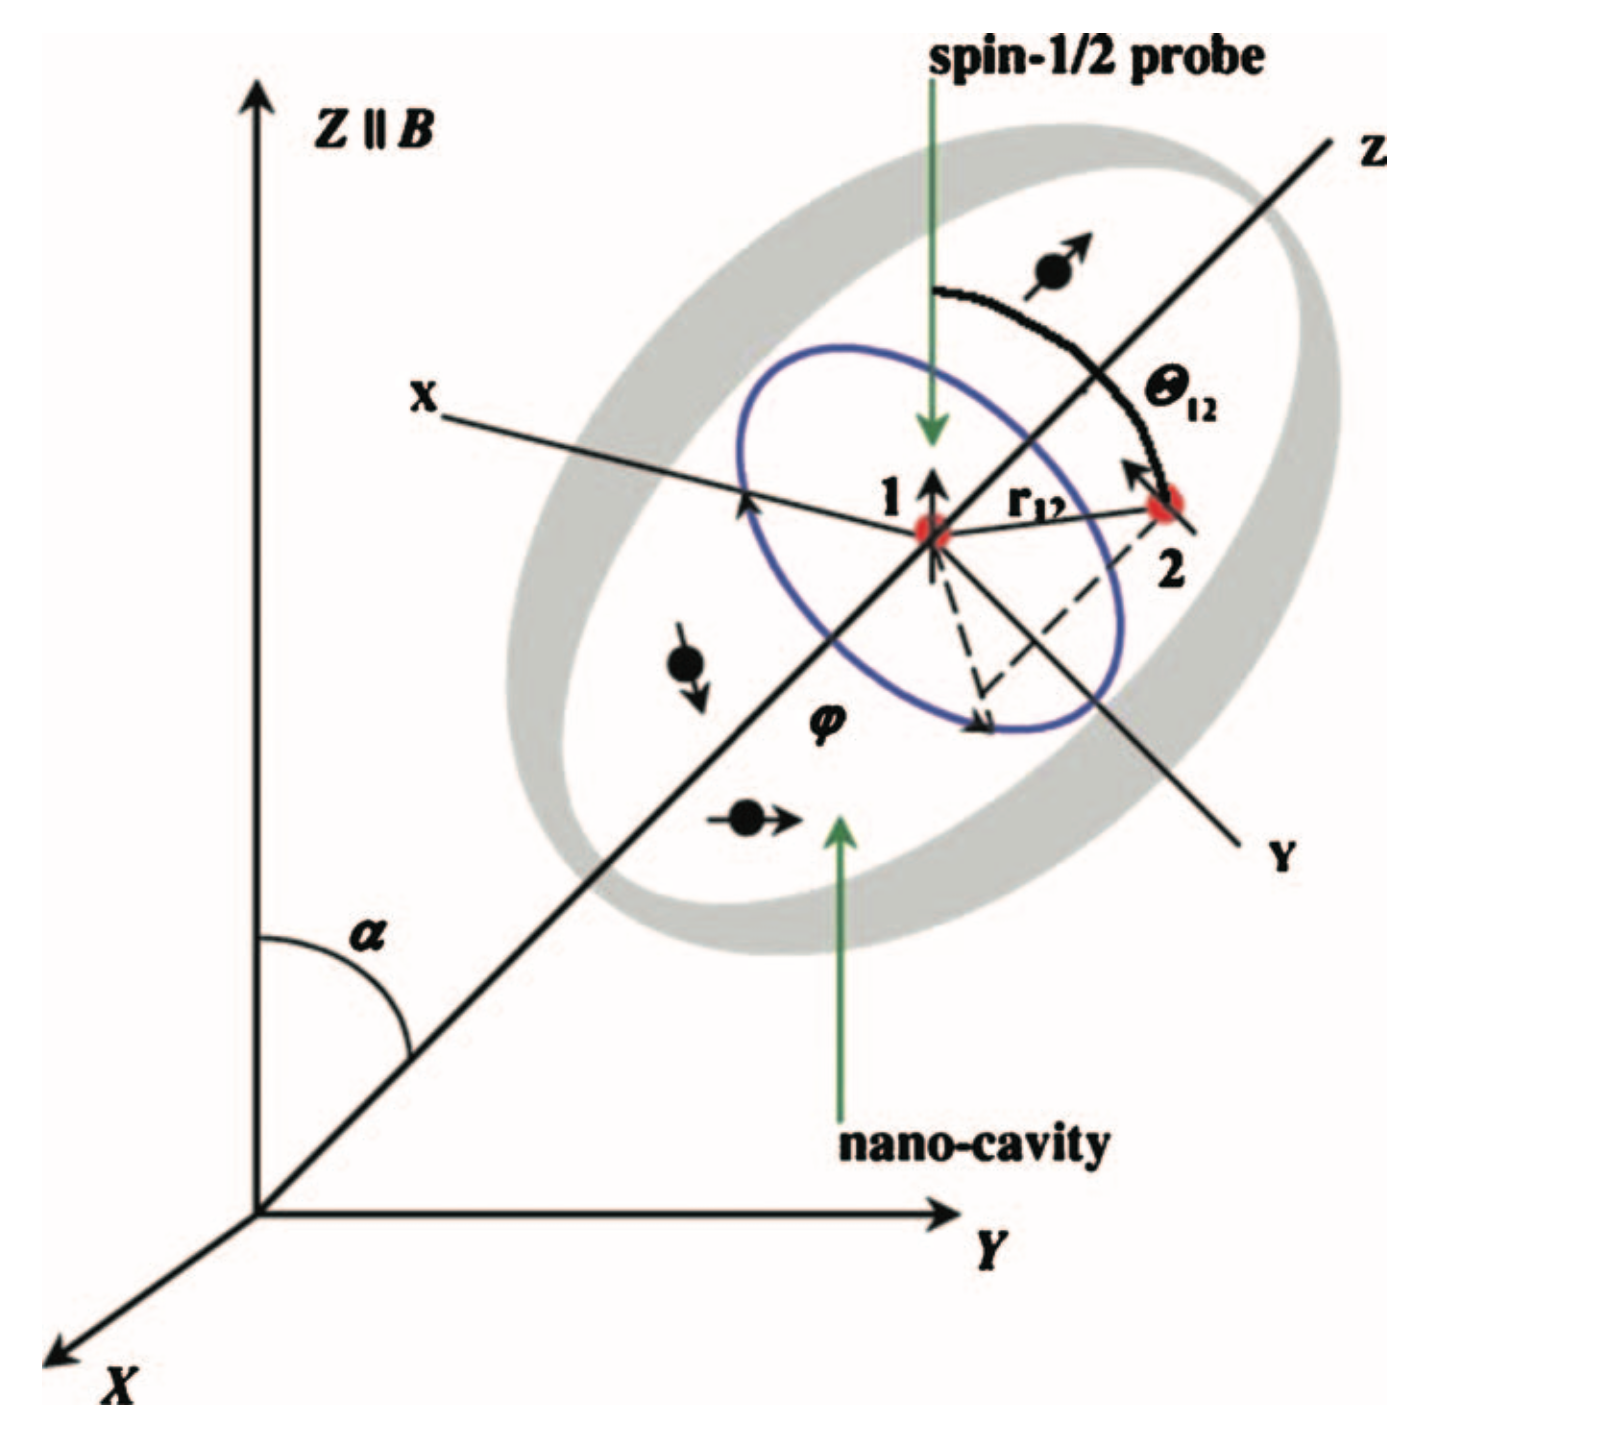
\includegraphics[width=\textwidth]{model-nanopore-schema.png}
  %   \caption{
  %     Hанопор~\cite{Baugh2001}
  %     со спин-несущих молекулами во внешнем сильном магнитном поле $\vec B$.
  %   }
  % \end{subfigure}
  % \hfill
  \begin{subfigure}[t]{0.55\textwidth}
    \centering
    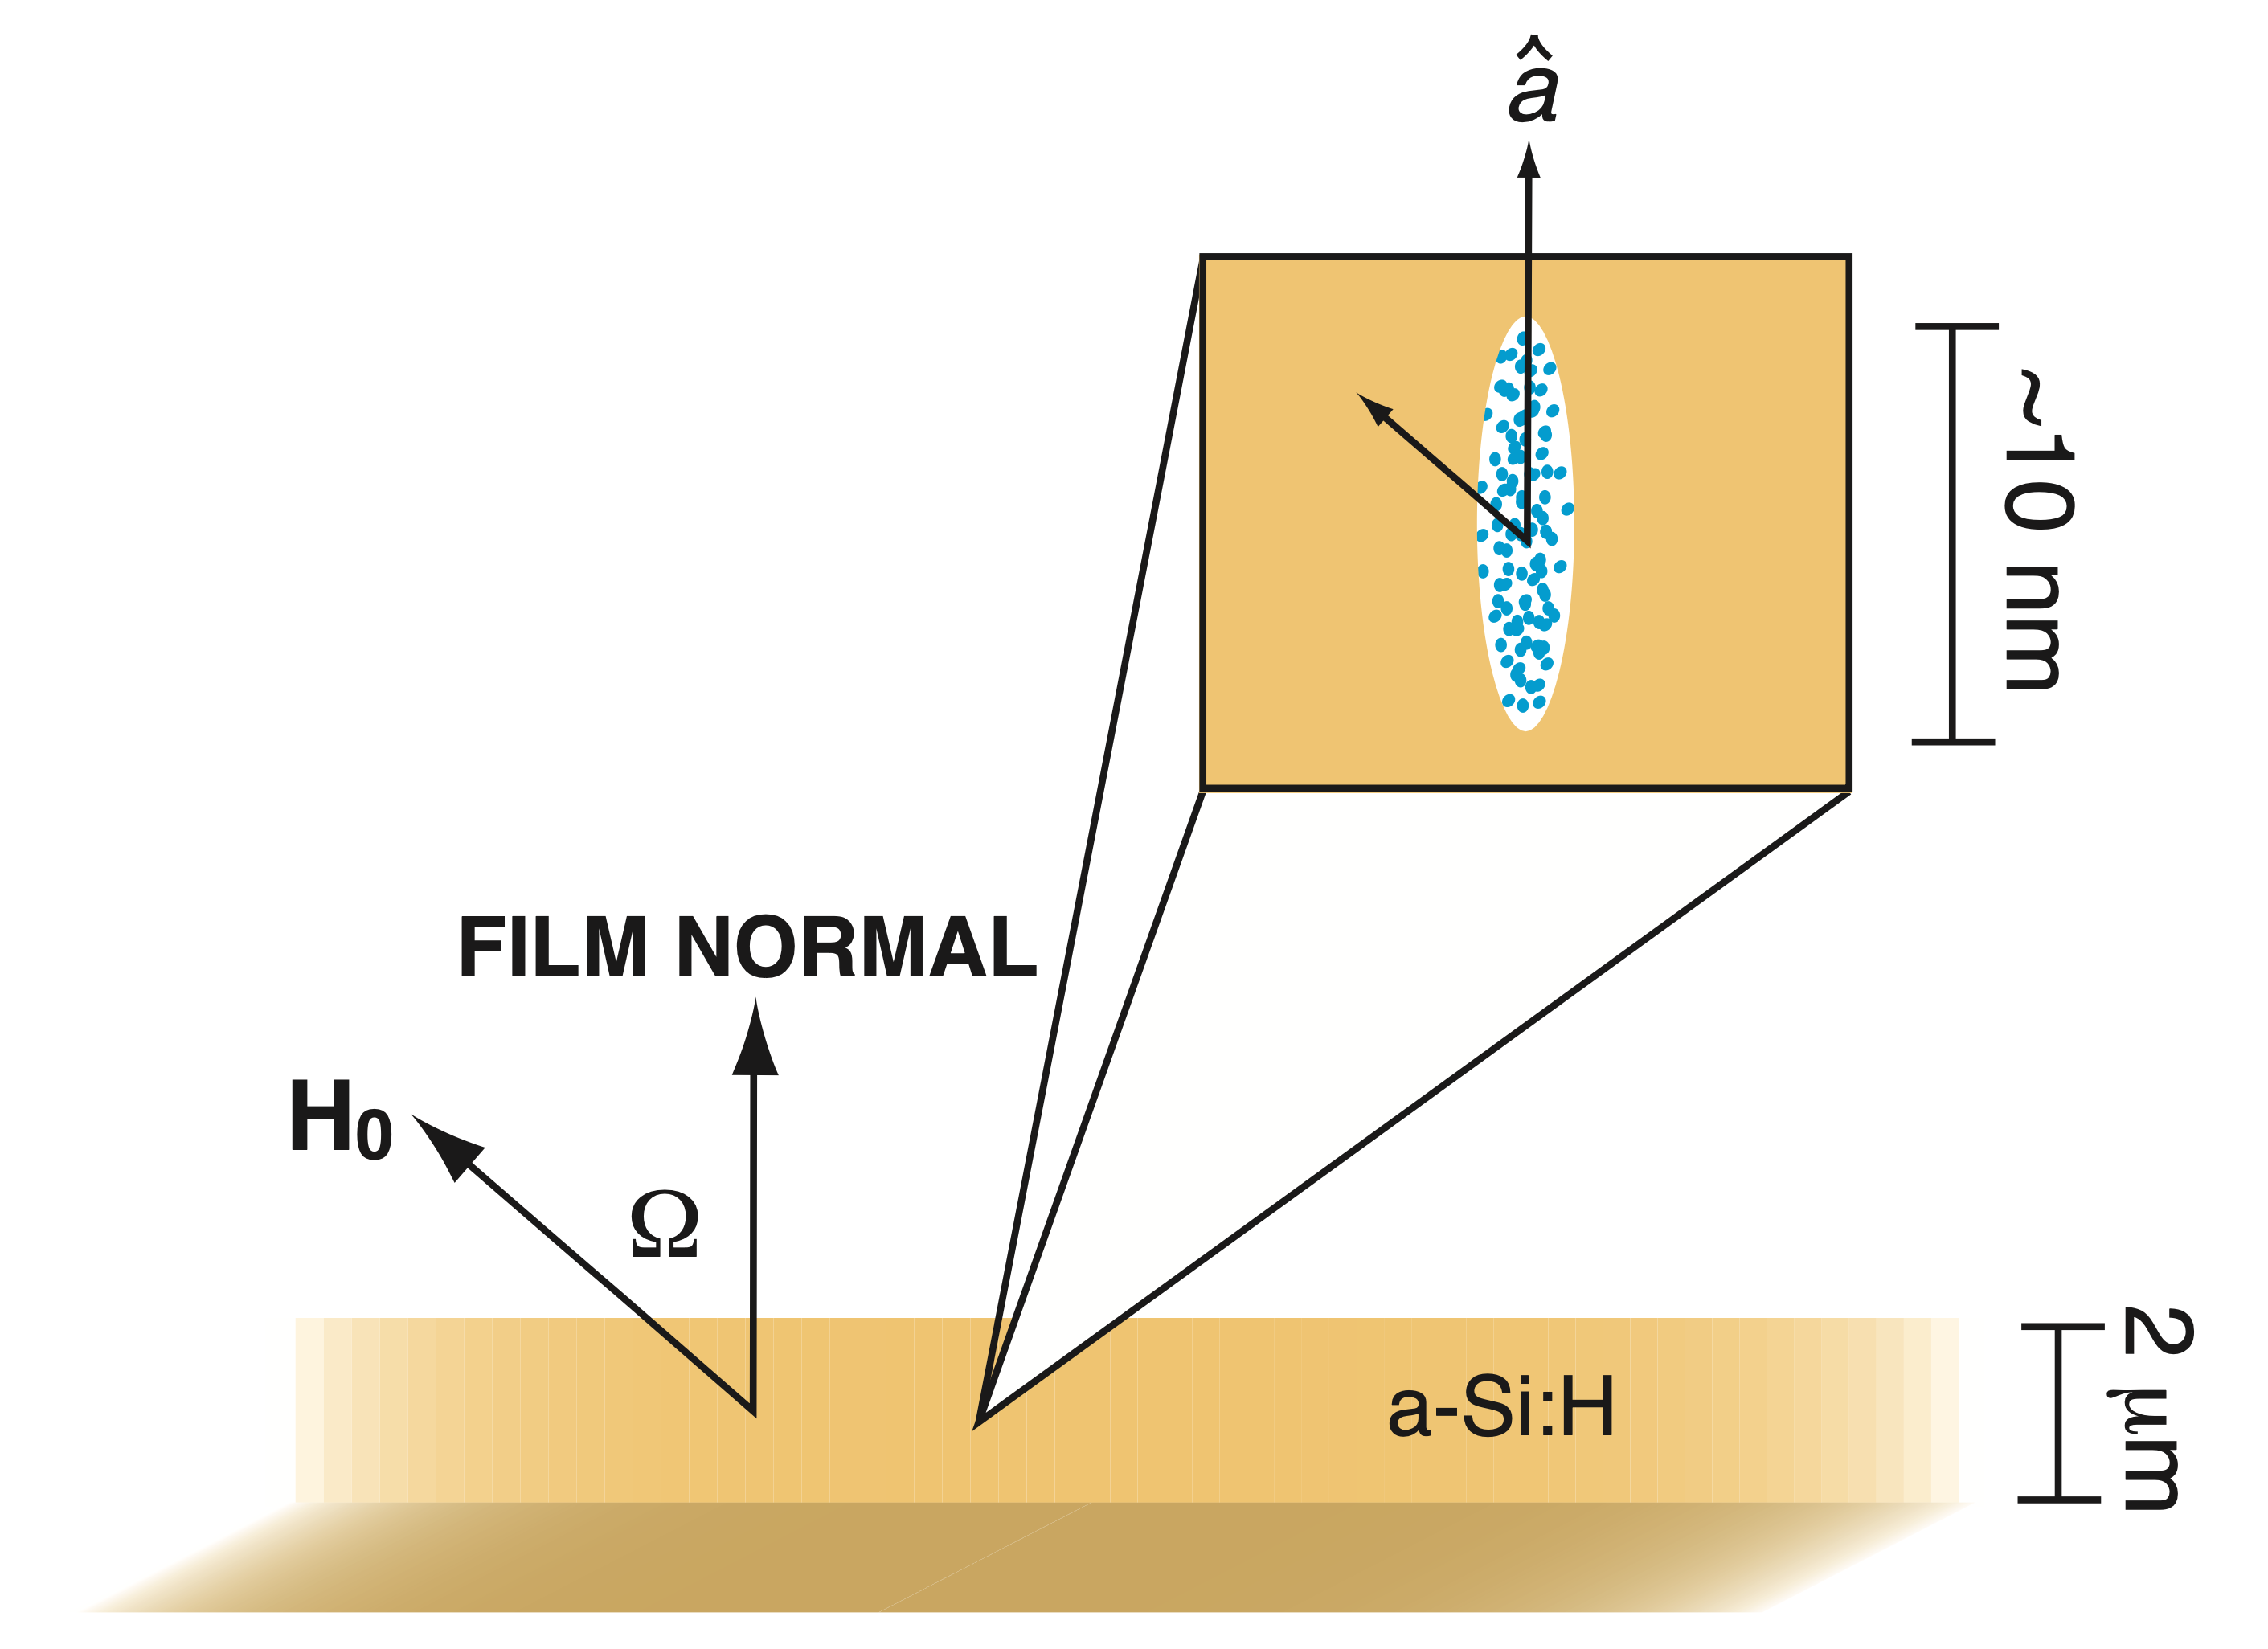
\includegraphics[width=\textwidth]{sample-nanopore-film.png}
    \caption{
      Иллюстрация поперечного сечения тонкой пленки гидрогенизированного аморфного кремния (a-Si:H) с увеличенной областью,
      показывающей вытянутую нанопору,
      содержащую газ H$_2$ высокой плотности (синие точки).
      Такие пустоты демонстрируют сильное выравнивание длинной оси по направлению роста (вдоль нормали пленки).
      Угол $\Omega$ --- это угол между внешним магнитным полем (H$_0$) и главной осью нанопоры.
    }
    \label{fig:sample-nanopore-film}
  \end{subfigure}
  \hfill
  \begin{subfigure}[t]{0.4\textwidth}
    \centering
    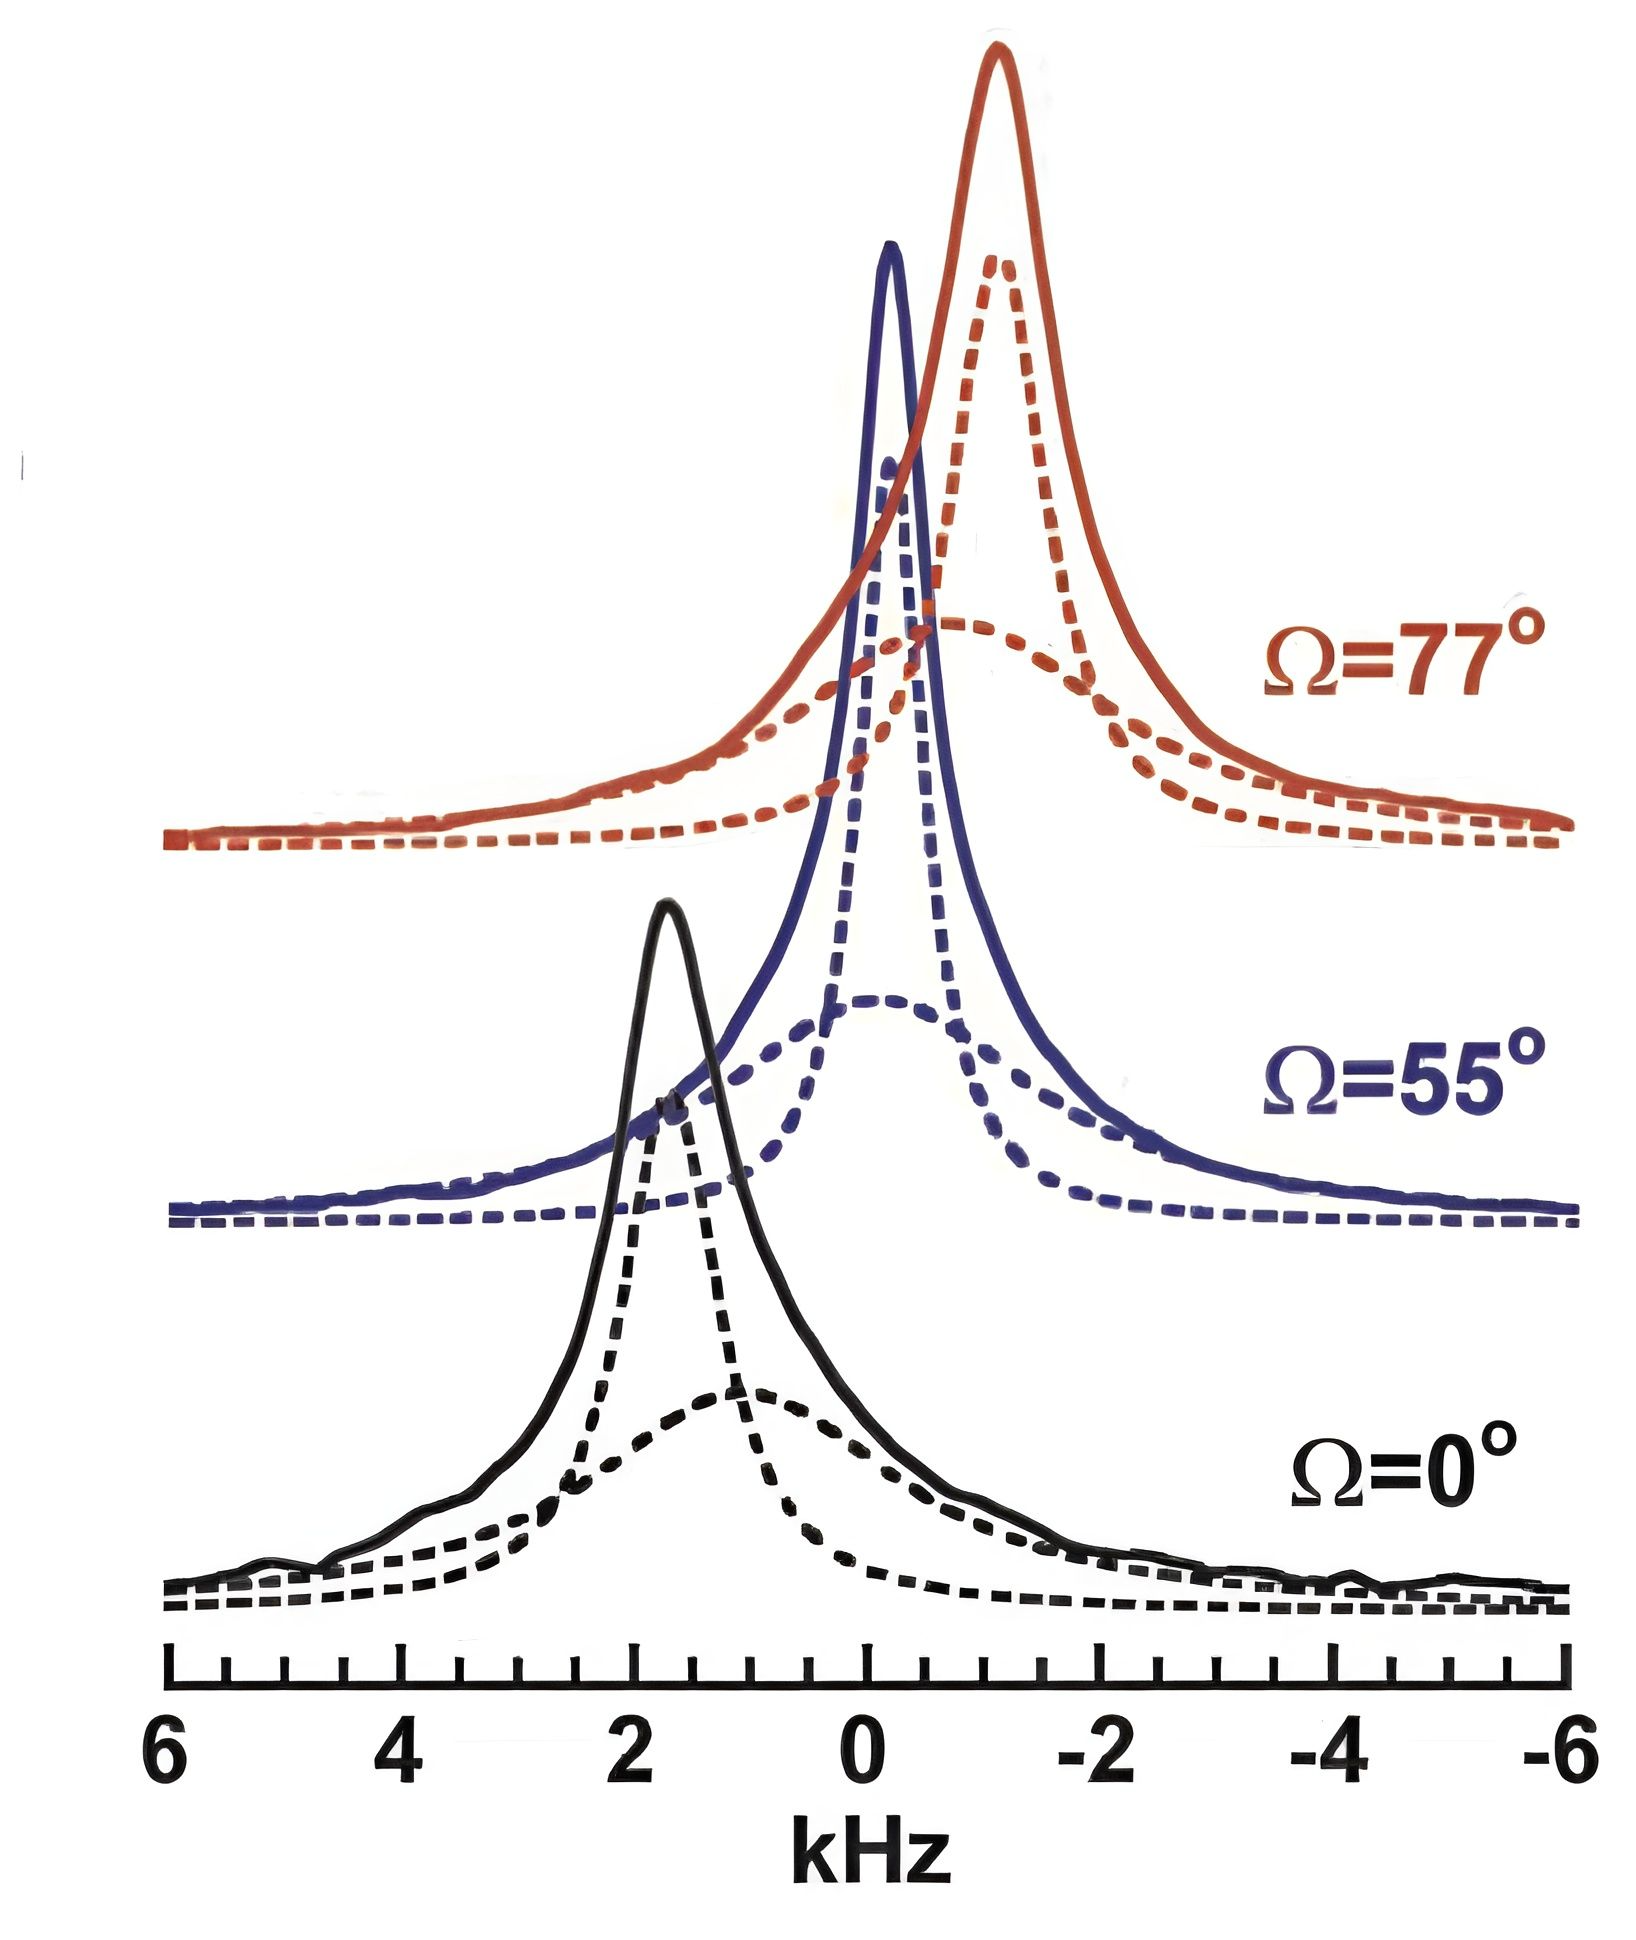
\includegraphics[width=\textwidth]{sample-nanopore-nmr-spectrum.png}
    \caption{
      Спектры ЯМР протонов при комнатной температуре (сплошные линии)
      и их линейные подгонки (пунктирные линии)
      для тонкой пленки a-Si:H,
      снятые при различных ориентациях пленки относительно приложенного магнитного поля (4,7 тесла).
      Угол определен на  Рис.~\ref{fig:sample-nanopore-film}.
      Значение константы связи $D$ зависит как от газа,
      так и от эффективного давления в нанопоре ($\approx 1$ кБар)
    }
    \label{fig:sample-nanopore-nmr-spectrum}
  \end{subfigure}
  % \captionsetup{skip=-0.1mm}
  \caption{}
\end{figure}


%PRA-2019
Для исследования многочастичной запутанности необходима такая модель взаимодействующих спинов,
в которой многоспиновая динамика может быть изучена при низких температурах.
Важно, чтобы модель содержала достаточно большое число спинов
и теория МК ЯМР была применима при произвольных температурах.
Только тогда можно исследовать многоспиновую запутанность и ее зависимость от температуры.
Несмотря на то, что уже разработана последовательная квантово-механическая теория МК динамики ЯМР для одномерных систем [20-22],
они плохо подходят для исследования многочастичной запутанности.
Дело в том, что точные решения для МК динамики ЯМР в одномерных системах показывают [20-22],
что, начиная с состояния термодинамического равновесия,
в приближении ближайших соседей возникают только нулевые и двойные квантовые когерентности.
В результате второй момент (дисперсия) МК спектра ЯМР мал и многоквантовая запутанность не возникает.
% Doronin2009jcp
Дальние взаимодействия приводят к когерентности более высокого порядка в МК спектрах ЯМР.
Однако эти взаимодействия находятся за пределами точных решаемых моделей [8-10].
Таким образом, необходимо применять численные методы
чтобы учесть дальние спин-спиновые связи.
Но даже суперкомпьютерные расчеты позволяют изучать МК динамику ЯМР спиновой цепочки,
состоящей не более чем из двадцати пяти спинов,
что недостаточно для исследования многочастичной запутанности в рамках МК динамики ЯМР.

Для исследования многоквантовой запутанности подходит модель эквивалентных спинов.
Примером такой модели является  несферическая нанопора [23],
заполненная газом спин-несущих атомов (например, ксеноном) (Рис.~\ref{fig:sample-nanopore-film})
или молекул в сильном внешнем магнитном поле.
Диполь-дипольные взаимодействия (ДДВ) спин-несущих атомов (молекул) в таких нанопорах не усредняются до нуля
в процессе молекулярной диффузии из-за несферичности нанопоры [23,24].
Остаточные усредненные ДДВ определяются только одной константой связи (Рис.~\ref{fig:sample-nanopore-nmr-spectrum}),
которая одинакова для всех пар взаимодействующих спинов [23,24].
Значение константы связи зависит как от газа,
так и от эффективного давления в нанопоре ($\approx 1$ кБар).
Это означает, что по существу мы имеем систему эквивалентных спинов.
Ниже будет показано, что МК динамика ЯМР такой системы может быть исследована точно~\cite{Doronin2009}.
Необходимо подчеркнуть,
что существуют некоторые ограничения для реализации описанной модели
при исследовании нанопористых соединений МК методами ЯМР.
Например, модель предполагает, что все нанопоры имеют одинаковый объем и одинаковую ``несферическую'' форму.


На подготовительном периоде МК эксперимента ЯМР (см. раздел~\ref{sec:mq-nrm-experiment})
МК динамика описывается усредненным несекулярный двухспиновый/двухквантовый гамильтонианом~(\ref{eq:hmq}).
Так как молекулярная диффузия газа значительнее бысрее дипольного взаимодействия с характерным временем [16]
%
\begin{equation}
  t \approx \omega^{-1}_\mathrm{loc},
  \quad
  \omega^2_\mathrm{loc} = \frac{\mathrm{Tr}(H^2_{dz})}{\mathrm{Tr}(I^2_z)}
\end{equation}
%
и периода многоимпульсной последовательности,
можно предположить,
что спиновая динамика описывается усредненной константой дипольной связи $D$,
которая одинакова для всех пар спинов.
Следовательно, многоквантовый гамильтониан системы может быть записан как
\begin{equation}\label{eq:mq-hamiltoninan-equivalent-spins}
  \bar H_\mathrm{MQ} = - \dfrac{D}{4} \left\{
      \left( I^{+} \right)^2 + \left( I^{-} \right)^2
  \right\},
\end{equation}
где $I^{+} = \sum\limits_{j=1}^{N} I^{\pm}_j$,
и $N$ --- число спинов в нанопоре.

Так как квадрат полного углового момента $\hat I^2$ коммутирует с
проекциями $I$ на произвольное направление,
следовательно, МК гамильтониан $\bar H_\mathrm{MQ}$ коммутирует с оператором квадрата полного углового момента
\begin{equation}\label{eq:hmq-i2-commutator}
  \left[ \bar H_\mathrm{MQ}, \hat I^2 \right] = 0
\end{equation}

Отметим так же,
что если $\lambda$ и $u$ собственное значение и собственный вектор  $\bar H_\mathrm{MQ}$,
то $-\lambda$ и $e^{-i\frac{\pi}{2}I_z}u$
так же являются собственным значением и собственным вектором соответственно.

Принимая во внимание свойство~(\ref{eq:hmq-i2-commutator}) и коммутационное соотношение ${[\hat I^2, I_z] = 0}$,
можно перейти к мультипликативному базису общих собственных состояний $\hat I^2$ и $I_z$.
Поскольку $\hat I^2$ сохраняется в МК эксперименте ЯМР
задача распадается на набор более простых задач для различных значений $\hat I^2$,
то есть в базисе собственных значений  $\hat I^2$ и $I_z$
гамильтониан $\bar H_\mathrm{MQ}$ имеет блочно-диагональный вид:
\begin{equation}
  \bar H_\mathrm{MQ} = \mathrm{diag} \left\{
    \bar H_\mathrm{MQ}^{N/2},
    \bar H_\mathrm{MQ}^{N/2 - 1},
    \dots
    \bar H_\mathrm{MQ}^{N/2 - [N/2]}
  \right\},
\end{equation}
где каждый блок соответствует собственному значению полного углового момента.

Для построения блока матрицы $H_\mathrm{MQ}^{S}$ необходимо определить ненулевые элементы операторов $I^{\pm}$.
Ненулевые элементы этих операторов, связанные с полным спиновым угловым моментом S
и имеют вид
%
\begin{equation}
  \bar{M}I^+\ket{M-1} = \bra{M-1}I^-\ket{M} = \sqrt{(S + M)(S - M + 1)},
\end{equation}
%
где $M = -S+1, -S+2, \dots, S-1, S$. Отсюда можно сделать вывод,
что
%
\begin{multline}\label{eq:i-square-elements}
  \bra{M}(I^+)^2\ket{M-2} = \bra{M-2}(I^-)^2\ket{M} \\
  = \sqrt{(S + M)(S + M -1)(S - M + 1)(S - M + 2)},
\end{multline}
%
где $M = -S+2, -S+3, \dots, S-1, S$,
а остальные элементы равны нулю.
Выражение~(\ref{eq:i-square-elements}) определяет ненулевые элементы блока гамильтониана $H_\mathrm{MQ}^{S}$.
Размер блока гамильтониана $H_{MQ}^S$ равен $2S+1$.
Полный размер гамильтониана, $2^N$,
может быть определен, как сумма размерностей всех блоков:
%
\begin{equation}\label{eq:full-dimension}
  \sum\limits_N n_N(S)(2S+1) = 2^N,
\end{equation}
%
где $n_N(S)$ --- это количество состояний системы из $N$ спинов
с фиксированным значением полного углового момента $S$,
которое может быть вычислено по формуле~\cite{Landau3}:
%
\begin{equation}\label{eq:coeff_n}
  n_N(S)  = \dfrac{ N! (2S+1)}
  {(\frac N 2 + S + 1)!(\frac N 2 - S)!},
  \quad
  0\leq S \leq \frac N 2.
\end{equation}
%

% Докажем выражение~(\ref{eq:full-dimension}),

% \subsection{Дипольно упорядоченное состояние}

\subsection{Измерение информации Фишера}
\label{sec:quantum-fisher-information-mesuarement-at-high-temperature}

% \subsection{Второй момент МК~спектра~ЯМР~как мера многоспиновой запутанности}
% \label{sec:4}
%
% Выражение~(\ref{eq:8}) для МК~сигнала~ЯМР~$G(\tau,\phi)$ может быть разложено в ряд по инкременту фазы импульсов
% %
% \begin{equation}
%   \begin{split}
%     \label{eq:17}
%     G(\tau,\phi)
%     & = \mathrm{Tr} \left\{
%       \rho(\tau) e^{i \phi I_\mathrm{z} }
%       \rho(\tau) e^{-i\phi I_\mathrm{z}}
%     \right\} \\
%     & = \mathrm{Tr} \left\{ \rho^2(\tau) \right\}
%     - \phi^2 \mathrm{Tr} \left\{
%       \rho^2(\tau) I^2_\mathrm{z}
%       - (\rho(\tau) I_\mathrm{z})^2
%     \right\}
%     + O(\phi^3)
%   \end{split}
% \end{equation}
% %
% Можно доказать~\cite{Girolami2017}, что квантовая информация Фишера $F_\mathrm{Q}(\rho,I_\mathrm{z})$~\cite{Helstrom1976} удовлетворяет неравенству:
% %
% \begin{equation}
%   \label{eq:18}
%   F_\mathrm{Q}(\rho,I_\mathrm{z}) \geq 4 \mathrm{Tr} \left\{ \rho^2 I^2_\mathrm{z} - (\rho I_\mathrm{z})^2 \right\}
% \end{equation}
% %
% В то же время легко проверить, что выражение $2 \mathrm{Tr} \left\{ \rho^2(\tau) I_\mathrm{z}^2 - \left( \rho(\tau) I_\mathrm{z} \right)^2 \right\}$ равно второму моменту $M_2$ распределения интенсивностей МК~когерентностей~ЯМР~\cite{Khitrin1997}
% %
% \begin{equation}
%   \label{eq:19}
%   M_2 = \sum_{n} n^2 J_n (\tau) ,
% \end{equation}
% %
% где $J_n(\tau)$ ($n=0,\pm 2, \pm 4, \cdots$) определяется уравнением~(\ref{eq:13}).
% Таким образом, второй момент распределения МК~интенсивностей~ЯМР~дает нижнюю границу квантовой информации Фишера $F_\mathrm{Q}(\rho,I_\mathrm{z})$.
% Также показано~\cite{T_th2014,Pezz2018}, что, если
% %
% \begin{equation}
%   \label{eq:20}
%   F_\mathrm{Q} (\rho,I_\mathrm{z}) > n k^2 + (N - n k)^2,
% \end{equation}
% %
% где $n$ - целая часть ${N/k}$, то система с матрицей плотности $\rho(\tau)$ содержит  $(k+1)$ запутанных спинов~\cite{Pezz2009,Hyllus2012,T_th2012}.
% Результаты численного анализа многоспиновой запутанности в системе спин-несущих молекул (атомов), первоначально приготовленных в дипольном упорядоченном состоянии, представлены в следующем разделе.
%
%
%

%
% % \begin{figure}
% %     \centering
% %     \includegraphics[width=\textwidth]{spin-system-energy-spectrum.png}
% %     \caption{Энергетический спектр системы}
% %     \label{fig:spectrum}
% % \end{figure}
%

% Начальная матрица плотности в МК ЯМР.
% %
% \begin{equation}
%     \label{eq:13}
%         \rho = \frac{1}{2}e^{\beta \omega_0 I_z} \approx
%             \frac{1}{z} \left(1 + \beta \omega_0 I_z \right)
% \end{equation}
% %
% В базисе, диагнолизирующем $\rho$, представляется в виде:
% %
% \begin{equation}
%     \label{eq:14}
%         \rho = \sum_k \lambda_k |k\rangle \langle k|
% \end{equation}
% %
% Энергетический спектр системы дан на Рис.~\ref{fig:spectrum}
%
%
%
% В ходе эволюции системы под действием гамильтониана
% %
% \begin{equation}
%     \label{eq:15}
%         H = H^{(2)} + H^{(-2)}
% \end{equation}
% %
% происходят переходы между энергетическими уровнями рис. 1 и возникают многоквантовые когерентности.
% Матрица плотности $\rho_t$ $(\theta\sim t)$ при этом имеет вид
% %
% \begin{equation}
%     \label{eq:16}
%         \rho_t = e^{-iHt}\rho e^iHt
% \end{equation}
%
% Формулы~(\ref{eq:14}),~(\ref{eq:16}) полнотью определяют квантовую информацию Фишера согласно формуле~(\ref{eq:12}).
%
% -----

% \begin{figure}
%     \centering
%     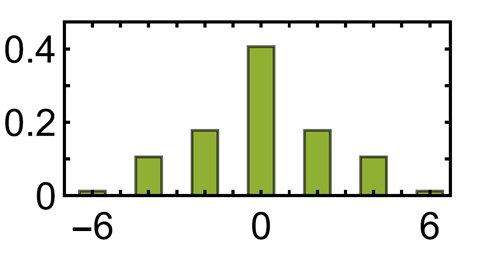
\includegraphics[width=\textwidth]{mq-coherence-intensities-hist.png}
%     \caption{Распределение интенсивности МК когерентностей ЯМР.}
%     \label{fig:distribution}
% \end{figure}
%

В разделе~\ref{sec:quantum-fisher-information} было показано,
что информацию Фишера можно интерпретировать как количественную оценку  запутанных частиц в системе.
Дальнейшее исследование многочастичной запутанности требует
разработки экспериментальных методов
для измерения квантовой информации Фишера.
В этом разделе будет показано,
что удвоенный второй момент распределения МК когерентностей ЯМР,
которые возникают на подготовительном периоде МК эксперимента ЯМР
(см. раздел~\ref{sec:mq-nrm-experiment}),
определяет нижнюю границу информации Фишера~\cite{Garttner2018}.

Пусть система в начальный момент времени находится в термодинамическом равновесии,
тогда матрица плотности системы имеет вид
%
\begin{equation}
  \label{eq:rho_eq}
  \rho(0)
  = \rho_{\mathrm{eq}}
  = \dfrac{
    e^{\frac{\hbar\omega_{0}}{kT} I_z}
  }{
    \tr{e^{\frac{\hbar\omega_{0}}{kT} I_z}}
  }
  \approx \dfrac{1}{2^N} (1 + bI_z)
  \sim I_z.
\end{equation}
%
Эволюционная матрица плотности на подготовительном периоде МК эксперимента ЯМР,
где динамика определяется стационарным МК гамильтонианом $H_\mathrm{MQ}$,
может быть выражена как
%
\begin{equation}\label{eq:rho_eval_ht}
  \rho_\mathrm{HT} (\tau)
   =  e^{-iH_\mathrm{MQ}\tau} I_z e^{iH_\mathrm{MQ}\tau}.
\end{equation}
%
С учетом Ур.~(\ref{eq:rho_eval_ht}) выражение~(\ref{eq:signal-after-mixing})
финального сигнала МК эксперимента ЯМР $G_\mathrm{HT}(\tau,\phi)$ можно переписать в виде
%
\begin{multline}\label{eq:signal-after-mixing-ht}
  G_\mathrm{HT}(\tau,\phi)
  = \tr{
  	e^{iH_{MQ}\tau} e^{i\phi I_z} e^{-iH_{MQ}\tau} I_z
  	e^{iH_{MQ}\tau} e^{-i\phi I_z} e^{-iH_{MQ}\tau} I_z
  }
  \\
  = \tr{
    e^{i\phi I_z} \rho_\mathrm{HT}(\tau)
    e^{-i\phi I_z}\rho_\mathrm{HT}(\tau)
  }.
\end{multline}
%
Из выражения~(\ref{eq:signal-after-mixing-ht}) следует,
что $G_\mathrm{HT}(\tau, \phi)$ является неупорядоченным по времени коррелятором ``out-of-time ordered correlator'' (OTOC)~\cite{Garttner2018, Doronin2019}.
Важно отметить, что данное свойство является ключевым в доказательстве связи
второго момента МК спектра ЯМР и квантовой информации Фишера.
Все дальнейшие рассуждения будут опираться на него.

Второй момент (дисперсия) $M_2(\tau)$ распределения интенсивностей МК когерентностей ЯМР может быть рассчитан из уравнения ~(\ref{eq:signal-after-mixing-ht})
\begin{equation}\label{eq:m2-derivative}
  M_2(\tau)
  = -\frac{1}{G_\mathrm{HT}(\tau, 0)}
    \frac{d^2 G_\mathrm{HT}(\tau, \phi)}{d\phi^2}\bigg|_{\phi=0}.
\end{equation}
%
Для этого разложим выражение~(\ref{eq:signal-after-mixing-ht})
для сигнала~$G_\mathrm{HT}(\tau,\phi)$ в ряд по инкременту фазы импульсов
%
% \begin{equation}\label{eq:17}
% \begin{split}
\begin{multline}
  G_\mathrm{HT}(\tau,\phi)
  = \tr{
    \rho_\mathrm{HT}(\tau) e^{i \phi I_\mathrm{z} }
    \rho_\mathrm{HT}(\tau) e^{-i\phi I_\mathrm{z}}
  } \\
  =  \tr{
    (1 - iI_z\phi - \frac{1}{2}I_z^2 \phi^2)
    \rho_\mathrm{HT}(\tau)
    (1 + iI_z\phi - \frac{1}{2}I_z^2 \phi^2)
    \rho_\mathrm{HT}(\tau)
  } \\
  = \tr{
    \rho_\mathrm{HT}^2
    - it [I_z,\rho_\mathrm{HT}(\tau)]
    + \phi^2 I_z \rho_\mathrm{HT}(\tau) I_z \rho_\mathrm{HT}(\tau)
    \\
    - \frac{\phi^2}{2}I_z^2 \rho_\mathrm{HT}^2(\tau)
    - \frac{\phi^2}{2} \rho_\mathrm{HT}(\tau) I_z^2 \rho_\mathrm{HT}(\tau)
  } \\
  = \tr{ \rho_\mathrm{HT}^2(\tau) }
  - \phi^2 \tr{
    \rho_\mathrm{HT}^2(\tau) I^2_\mathrm{z}
    - (\rho_\mathrm{HT}(\tau) I_\mathrm{z})^2
  }
  + O(\phi^3)
% \end{split}
% \end{equation}
\end{multline}
%
Отсюда второй момент распределения МК когерентностей ЯМР
%
\begin{equation}\label{eq:m2-trace}
  M_{2,\mathrm{HT}}(\tau) = 2 \tr{
    \rho_\mathrm{HT}(\tau)^2 I_z^2
    - \rho_\mathrm{HT}(\tau) I_z \rho_\mathrm{HT}(\tau) I_z
  },
\end{equation}
%
так как в МК эксперименте ЯМР сумма всех интенсивностей нормируется на 1
и
\begin{equation}\label{eq:mq-coherences-sum}
  G_\mathrm{HT}(\tau, 0)
  = \tr{\rho_\mathrm{HT}(\tau)^2}
  = \tr{\sum\limits_{n,m} \rho_n \rho_m}
  = \tr{\sum\limits_{n} \rho_n \rho_n}
  = \sum_n J_n (\tau) \equiv 1,
\end{equation}
где $\rho_n$ --- это вклад МК когерентности $n$-ого порядка в матрицу плотности $\rho_\mathrm{HT}(\tau)$,
а $J_n$ --- интенсивность МК когерентности $n$-ого порядка.
%
Выражение~(\ref{eq:m2-trace}) для второго момента $M_{2,\mathrm{HT}}(\tau)$
может быть выражено через собственные значения $\lambda_i$ матрицы плотности $\rho_\mathrm{HT}(\tau)$:
%
\begin{equation}\label{eq:m2-via-lambdas}
\begin{split}
  M_{2,\mathrm{HT}}(\tau)
  &= 2 \sum_{j,k}\p{\lambda^2_j (I_z)_{jk} (I_z)_{kj} - \lambda_j (I_z)_{jk} \lambda_k (I_z)_{kj}}
  \\
  &= 2 \sum_{j,k} (\lambda^2_j - \lambda_j \lambda_k) (I_z)_{jk} (I_z)_{kj}
  \\
  &= \sum_{j,k} (\lambda^2_j - \lambda_j \lambda_k) (I_z)_{jk} (I_z)_{kj}
    + \sum_{j,k} (\lambda^2_j - \lambda_j \lambda_k) (I_z)_{kj} (I_z)_{jk}
  \\
  &= \sum_{j,k}
    (\lambda^2_j - 2\lambda_j \lambda_k + \lambda^2_k)
    (I_z)_{kj} (I_z)_{jk}
  \\
  &= \sum_{j,k}
    (\lambda_j - \lambda_k)^2
    \left| \bra{j} I_z \ket{k} \right|^2
\end{split}
\end{equation}
%
По определению~\ref{def:quantum-fisher-information} квантовая информация Фишера дается выражением
\begin{equation}
    F_Q(\rho_\mathrm{HT}(\tau), I_z) = 2\sum_{j,k} \frac{(\lambda_j - \lambda_k)^2}{\lambda_j + \lambda_k}
    \left| \bra{j} I_z \ket{k} \right|^2.
\end{equation}
Поскольку $\tr{\rho_\mathrm{HT}} = 1$, $\lambda_j + \lambda_k \leq 1$ и
%
\begin{equation}\label{eq:qfi-low-bound}
  F_Q(\rho_\mathrm{HT}(\tau), I_z) \geq 2\sum_{j,k} (\lambda_j - \lambda_k)^2 \left| \bra{j} I_z \ket{k} \right|^2
\end{equation}
%
Из выражений~(\ref{eq:qfi-low-bound})~и~(\ref{eq:m2-via-lambdas}) следует, что
\begin{equation}
  F_Q(\rho_\mathrm{HT}(\tau), I_z) \geq M_{2,\mathrm{HT}}(\tau)
\end{equation}
%
Таким образом, нижняя граница информации Фишера равна удвоенному второму моменту.

Данный результат получен в случае высоких зеемановских температур,
когда начальное состояние системы $I_z$.
В свою очередь квантовые корреляции преимущественно возникают при температурах близких к нулю,
поэтому исследование многочастичной запутанности этим методом невозможно.
В следующей главе~\ref{chapter:quantum-fisher-information-measurement}
будет предложено такое обобщение МК эксперимента ЯМР,
которое позволить измерять информацию Фишера при произвольной температуре.

%   \section{Выводы}
%   ЯМР являтся отличным инструментом для исседования квантовых систем
% Мы можем заключить, что спектроскопия MQ ЯМР
% является эффективным методом для исследования многоспиновой запутанности
% и распространения МК корреляций внутри многоспиновых систем.
% Он может быть использован для экспериментальных исследований квантовой обработки информации в твердых телах (обратите внимание на соответствующее исследование декогеренции в жидкостях \cite{HOU2017863}).

% Проведенные исследования позволяют заключить, что МК~спектроскопия~ЯМР~является тонким и полезным методом для исследования различных проблем квантовой информатики.
% В частности, это очень эффективный метод исследования квантовой запутанности.
% \chapter{Измерение квантовой информации Фишера в МК эксперименте ЯМР}
\chapter{Измерение информации Фишера в МК эксперименте ЯМР}
\label{chapter:quantum-fisher-information-measurement}
% (PRA-2019)
% - Расчет динамики при низкой температуре
% - Вычисление второго момента

В разделе~\ref{sec:quantum-fisher-information-mesuarement-at-high-temperature}
была обсуждена связь между вторым моментом распределения интенсивностей МК когерентностей ЯМР и квантовой информацией Фишера~\cite{Toth2014,Pezze2018}.
В частности, было показано,
что в классическом эксперименте ЯМР, когда сигнал усредняется по наблюдаемой $I_z$, в области высоких температур второй момент МК спектра соответствует нижней границе квантовой информации Фишера~\cite{Garttner2018}.
Ниже будет показано, что МК эксперимент ЯМР может быть проведен таким образом,
что связь квантовой информации Фишера и второго момента сохранится для произвольных температур.


\section{МК динамика ЯМР при низких температурах}
%\section{МК когерентности ЯМР}
\begin{figure}[H]
  \centering
  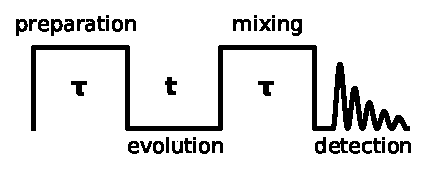
\includegraphics[width=0.5\textwidth]{mq-experiment-schema.pdf}
  \caption{Схема МК эксперимента ЯМР}
  \label{fig:mq-experiment-schema}
\end{figure}

Первоочередно рассмотрим теорию МК динамики ЯМР (см. раздел~\ref{sec:mq-nrm-experiment})
для термодинамически равновесного начального состояния системы $\rho_\mathrm{eq}$,
которое определяется выражением
%
\begin{equation}
  \label{eq:rho_eq}
  \rho_{\mathrm{eq}} = \dfrac{e^{\frac{\hbar\omega_{0}}{kT} I_z}}{Z},
\end{equation}
%
где $Z =\mathrm{Tr}\left\{e^{\frac{\hbar\omega_{0}}{kT} I_z}\right\}$ это статистическая сумма,
$\hbar$ и $k$ --- это постоянная Планка и постоянная Больцмана,
$\omega_0$ --- Ларморовская частота,
$T$ --- температура,
и $I_z$ это оператор проекции полного углового момента на ось $z$,
которая направлена вдоль сильного внешнего магнитного поля.

Для теоретического исследования МК динамики ЯМР
необходимо найти эволюционную матрицу плотности $\rho(\tau)$
на подготовительном периоде МК эксперимента ЯМР (см. раздел~\ref{sec:mq-nrm-experiment}),
решив уравнение Лиувилля~\cite{Feldman2012}
%
\begin{equation}
    \label{eq:liouvile}
    i \dfrac{d\rho(\tau)}{d \tau} =
    \left[H_\mathrm{MQ}, \rho(\tau)\right].
\end{equation}
%
с начальной матрицей плотности $\rho(0)$,
находящейся в термодинамическом равновесии,
%
\begin{equation}
    \label{eq:rho_init}
    \rho(0) = \rho_{\mathrm{eq}}.
\end{equation}
%
Так как в рассматриваемом случае гамильтониан~$H_\mathrm{MQ}$
не зависит от времени,
эволюционная матрица плотности может быть выражена как
\begin{equation}
  \label{eq:rho_eval_lt}
  \rho_\mathrm{LT} (\tau) = e^{-iH_\mathrm{MQ}\tau} \rho_\mathrm{eq} e^{iH_\mathrm{MQ}\tau},
\end{equation}
В области высоких температур,
когда $b = \frac{\hbar\omega_{0}}{kT} \ll 1$,
начальную матрицу плотности $\rho_{\mathrm{eq}}$ можно разложить в ряд по $b$:
%
\begin{equation}
  \label{eq:rho_ht}
  \rho_{\mathrm{eq}} \approx \dfrac{1}{2^N} (1 + bI_z).
\end{equation}
%
В этом случае эволюционную матрицу плотности можно переписать, как
\begin{equation}\label{eq:rho_eval_ht}
  \rho_\mathrm{HT} (\tau) =  e^{-iH_\mathrm{MQ}\tau} I_z e^{iH_\mathrm{MQ}\tau},
\end{equation}

Экспериментальное исследование МК динамики ЯМР заключается в проведении
МК эксперимента ЯМР (см. раздел~\ref{sec:mq-nrm-experiment})
и последующем измерении интенсивностей МК когерентностей ЯМР.
В результате проведения всех периодов МК эксперимента ЯМР (Рис.~\ref{fig:mq-experiment-schema})
итоговый сигнал $G(\tau, \phi)$ хранится в информации о населенности\cite{Feldman1997}.
Выражение для сигнала $G(\tau, \phi)$ имеет вид
%
\begin{equation}
  \label{eq:signal}
   G(\tau, \phi)
   = \tr{
     e^{iH_\mathrm{MQ}\tau} e^{i\phi I_z} e^{-iH_\mathrm{MQ}\tau}
     \rho_\mathrm{eq}
     e^{iH_\mathrm{MQ}\tau} e^{-i\phi I_z} e^{-iH_\mathrm{MQ}\tau}
     I_z
    }.
\end{equation}
%
Перегруппировкой множителей,
выражение~(\ref{eq:signal}) может быть переписано через
 $\rho_\mathrm{LT} (\tau)$ и $\rho_\mathrm{HT} (\tau)$:
%
\begin{equation}
  \label{eq:signal-short}
  G(\tau, \phi) = \tr{
   e^{i\phi I_z} \rho_\mathrm{LT} (\tau)
   e^{-i\phi I_z} \rho_\mathrm{HT} (\tau).
  }
\end{equation}


Для получения выражений сигналов отдельных когерентностей,
перейдем к представлению матриц плотности
$\rho_\mathrm{LT} (\tau)$ и $\rho_\mathrm{HT} (\tau)$
в виде ряда
%
\begin{equation}\label{eq:rho_series}
  \rho_\mathrm{LT} (\tau) = \sum_n \rho_{LT, n}(\tau); \quad
  \rho_\mathrm{HT} (\tau) = \sum_n \rho_{HT, n}(\tau),
\end{equation}
%
где $\rho_{LT, n} (\tau)$ и  $\rho_{HT, n} (\tau)$
это вклад МК когерентности $n$-ого порядка
в матрицы плотности $\rho_\mathrm{LT} (\tau)$ и $\rho_\mathrm{HT} (\tau)$ соответственно.
Подставляя~(\ref{eq:rho_series}) в~(\ref{eq:signal}) итоговый сигнал $G(\tau, \phi)$ МК когерентностей ЯМР можно переписать как
%
\begin{equation}
    \label{eq:signal_series}
    G(\tau, \phi) = \sum\limits_n
    e^{in\phi}\mathrm{Tr} \left\{
    \rho_{LT, n}(\tau) \rho_{HT, -n} (\tau)
    \right\},
\end{equation}
%
где учтены коммутационные соотношения
%
\begin{equation}
    \left[I_z, \rho_{LT, n} (\tau) \right] = n  \rho_{LT, n} (\tau);
    \quad
    \left[I_z, \rho_{HT, n} (\tau) \right] = n  \rho_{HT, n} (\tau).
\end{equation}

Нормированные интенсивности МК когерентностей ЯМР могут быть выражены следующим образом
%
\begin{equation}
    \label{eq:coherence}
    J_n(\tau)
    = \dfrac{
       \mathrm{Tr} \left\{
        \rho_{LT, n}(\tau) \rho_{HT, -n} (\tau)
        \right\}
    }{Tr \left\{\rho_{\mathrm{eq}}I_z\right\}}.
    = \dfrac{
       \mathrm{Tr} \left\{
        \rho_{LT, n}(\tau) \rho_{HT, -n} (\tau)
        \right\}
    }{\frac N 2 \tanh \frac b 2}.
\end{equation}

МК когерентности ЯМР имеют несколько свойств.
Во-первых, в момент времени  $\tau=0$
нормированная интенсивность $J_0(0)$ МК когерентности ЯМР нулевого порядка равна 1,
а остальные интенсивности равны нулю.
Во-вторых, сумма всех нормированных когерентностей равна единице.
Докажем это утверждение.
Используя выражения~(\ref{eq:rho_eq}) и~(\ref{eq:rho_eval_ht})
выразим $\rho_\mathrm{LT}(\tau)$ через $\rho_\mathrm{HT}(\tau)$.
%
\begin{equation}\label{eq:lt-through-ht}
  \rho_\mathrm{LT}(\tau) = \dfrac 1 Z
  \exp\left(be^{-iH_\mathrm{MQ}\tau} I_z e^{iH_\mathrm{MQ}\tau}\right) =
  \dfrac 1 Z e^{b\rho_\mathrm{HT}(\tau)}.
\end{equation}
%
Подставляя выражение~(\ref{eq:lt-through-ht}) в~(\ref{eq:coherence}) получаем
%
\begin{multline}
  \label{eq:sum_of_coherence}
  \sum\limits_n J_n(\tau) =
  \dfrac{\sum\limits_{n, m}\mathrm{Tr}\left\{
      \rho_{LT, n}(\tau)\rho_{HT, m}(\tau)
  \right\}}
  {\mathrm{Tr}\left\{\rho_\mathrm{eq} I_z\right\}} = \\
  \dfrac{\mathrm{Tr}\left\{
      \rho_\mathrm{LT}(\tau)\rho_\mathrm{HT}(\tau)
  \right\}}
  {\mathrm{Tr}\left\{\rho_\mathrm{eq} I_z\right\}} =
  \dfrac{\mathrm{Tr}\left\{
      \rho_\mathrm{HT}(\tau)e^{b\rho_\mathrm{HT}(\tau)}
  \right\}}
  {Z\mathrm{Tr}\left\{\rho_\mathrm{eq} I_z\right\}} = \\
  \dfrac{\frac{d}{db} \ln \mathrm{Tr}\left\{
      e^{b I_z}
  \right\}}
  {\mathrm{Tr}\left\{\rho_\mathrm{eq} I_z\right\}} =
  \dfrac{\frac 1 2 N \tanh \left( \frac b 2 \right)}
  {\frac 1 2 N \tanh \left( \frac b 2 \right)} = 1.
\end{multline}
Ур.~(\ref{eq:sum_of_coherence}) подтверждает,
что сумма МК когерентностей ЯМР сохраняется на подготовительном периоде МК эксперимента ЯМР.


\section{Приведенные МК когерентности ЯМР}
\label{sec:reduced-mq-coherences}

В предыдущем разделе было получено выражение~(\ref{eq:signal-short}) коррелятора сигнала $G(\tau, \phi)$,
которое в области высоких температур имеет вид
%
\begin{equation}
    \label{eq:otoc-ht}
    G_\mathrm{HT}(\tau, \phi) = \frac b Z\mathrm{Tr}\left\{
    e^{i \phi I_z}
    \rho_\mathrm{HT} (\tau)
    e^{-i \phi I_z}
    \rho_\mathrm{HT}(\tau)
    \right\},
\end{equation}
%
так как согласно разложению~(\ref{eq:rho_ht})
%
\begin{equation}
  \rho_\mathrm{LT} (\tau) \approx \frac 1 Z + \frac b Z \rho_\mathrm{HT}.
\end{equation}
%
Так же в разделе~\ref{sec:quantum-fisher-information-mesuarement-at-high-temperature}
было отмечено,
что связь второго момента МК спектра ЯМР и квантовой информации Фишера
обеспечивается благодаря особому виду коррелятора сигнала.
% Коррелятор должен принадлежать классу неупорядоченных по времени корреляторов ``out-of-time-ordered correlator'' (OTOC).
Выражение~(\ref{eq:otoc-ht}) для $G_\mathrm{HT}(\tau, \phi)$
в высоко температурной области
удовлетворяет этому требованию,
в отличие от выражения~(\ref{eq:signal-short}) для $G(\tau, \phi)$.
$G(\tau, \phi)$ не является неупорядоченным по времени коррелятором,
так как выражение~(\ref{eq:signal}) содержит разные матрицы $\rho_\mathrm{LT}(\tau)$ и $\rho_\mathrm{HT}(\tau)$.
Однако можно обобщить МК эксперимент ЯМР  таким образом,
чтобы привести сигнал $G(\tau, \phi)$ к нужному виду.
Для достижения такого поведения коррелятора финального сигнала МК эксперимента ЯМР
необходимо усреднить сигнал,
полученный после трех периодов %МК эксперимента ЯМР
(Рис.~\ref{fig:mq-experiment-schema}),
по начальному состоянию $\rho_\mathrm{eq}$.
Тогда коррелятор сигнала будет описываться следующим выражением
%
\begin{multline}
  \label{eq:otoc_LT}
  G_\mathrm{LT}(\tau, \phi) =
  \mathrm{Tr}\left\{
    e^{i H_{\mathrm{MQ}} \tau}
    e^{i \phi I_z}
    e^{-i H_{\mathrm{MQ}} \tau}
    \rho_{\mathrm{eq}}
    e^{i H_{\mathrm{MQ}}}
    e^{-i \phi I_z}
    e^{-i H_{\mathrm{MQ}} \tau}
    \rho_{\mathrm{eq}}
  \right\} \\ =
  \mathrm{Tr}\left\{
    e^{i \phi I_z}
    e^{-i H_\mathrm{MQ} \tau}
    \rho_\mathrm{eq}
    e^{i H_\mathrm{MQ} \tau}
    e^{-i \phi I_z}
    e^{-i H_\mathrm{MQ} \tau}
    \rho_{\mathrm{eq}}
    e^{i H_\mathrm{MQ} \tau}
  \right\} \\ =
  \mathrm{Tr}\left\{
    e^{i \phi I_z}
    \rho_\mathrm{LT} (\tau)
    e^{-i \phi I_z}
    \rho_\mathrm{LT} (\tau)
  \right\}.
\end{multline}
%
Из выражения~(\ref{eq:otoc_LT}) следует,
что $G_\mathrm{LT}(\tau, \phi)$ является неупорядоченным по времени коррелятором при произвольных температурах.
Важно отметить,
что полученный результат для начальной матрицы~(\ref{eq:rho_eq}) легко обобщить
на произвольное начальное состояние.
Связь квантовой информации Фишера и второго момента будет выполняться всегда,
если по итогу трех периодов (Рис.~\ref{fig:mq-experiment-schema}) МК экскремента ЯМР
проводить усреднение по начальному состоянию.
Это наблюдение будет играть важную роль в следующей Главе~\ref{chapter:manyparticle-entanglement-in-nanopore}
при рассмотрении МК динамики ЯМР дипольных упорядоченных состояний.

Нормированные интенсивности МК когерентностей ЯМР для сигнала $G_\mathrm{LT}(\tau, \phi)$
могут быть записаны по аналогии с~(\ref{eq:coherence}):
%
\begin{equation}\label{eq:reduced-mq-coherences}
    J_{\mathrm{LT}, n}(\tau) =
    \frac{\mathrm{Tr} \left\{
        \rho_{\mathrm{LT},n}(\tau)
        \rho_{\mathrm{LT}, -n}(\tau)
    \right\}}
    {\mathrm{Tr}\left\{\rho^2_\mathrm{eq}\right\}}.
\end{equation}
%
В этом случае нормировочный член определяется как
%
\begin{equation}\label{eq:j_lt_norm}
  \mathrm{Tr}\left\{\rho^2_\mathrm{eq}\right\} =
    \frac{2^N \cosh^N(b)}{Z^2}.
\end{equation}
Когерентности определяемые выражением~(\ref{eq:reduced-mq-coherences})
являются приведенными МК когерентностями ЯМР.
%
Используя разложение~(\ref{eq:rho_series}),
сумма интенсивностей приведенных МК когерентностей ЯМР~(\ref{eq:reduced-mq-coherences}) может быть записана как
%
\begin{multline}\label{eq:reduced-coherences-sum}
  \sum\limits_{n} J_{\mathrm{LT}, n}(\tau)
  = \dfrac{
    \tr{
      \sum\limits_{n}
      \rho_{\mathrm{LT}, n}(\tau)
      \rho_{\mathrm{LT},-n}(\tau)}
    }{
    \tr{\rho^2_\mathrm{eq} }
  }
  = \dfrac{
    \tr{
      \sum\limits_{m,n}
      \rho_{\mathrm{LT}, n}(\tau)
      \rho_{\mathrm{LT}, m}(\tau)
    }}{
    \tr{\rho^2_\mathrm{eq}}
  }
  \\
  = \dfrac{
    \tr{\rho_\mathrm{LT}^2(\tau)}
  }{
    \tr{\rho^2_\mathrm{eq}(\tau)}
  }
  = \dfrac{
    \tr{
      e^{-i H_\mathrm{MQ} \tau}
      \rho^{2}_\mathrm{eq}
      e^{i H_\mathrm{MQ} \tau}
    }
  }{
    \tr{ \rho^2_\mathrm{eq}}
  }
  = 1.
\end{multline}
%
Из уравнения~(\ref{eq:reduced-coherences-sum}) можно сделать вывод, что сумма МК~когерентностей~ЯМР~сохраняется на подготовительном периоде МК~эксперимента~ЯМР~\cite{Baum1985}.


Удвоенный второй момент (дисперсия) $M_2(\tau)$ распределения интенсивностей приведенных МК когерентностей ЯМР $J_{\mathrm{LT}, n} (\tau)$
является нижней границей квантовой информации Фишера $F_{Q}$
(см. раздел~\ref{sec:quantum-fisher-information-mesuarement-at-high-temperature}):
\begin{equation}\label{eq:fisher-low-bound}
  F_{Q}(\tau) \geq 2M_2(\tau),
\end{equation}
где второй момент может быть выражен~\cite{Khitrin1997} как
%
\begin{equation}\label{eq:m2-via-coherences}
  M_2(\tau) = \sum\limits_n n^2 J_{\mathrm{LT}, n} (\tau).
\end{equation}

\section{Выводы}
В этой главе было предложено обобщение МК эксперимента ЯМР,
позволяющее измерять нижнюю границу квантовой информации Фишера
в произвольный момент времени подготовительного периода МК эксперимента ЯМР
с произвольным начальным состоянием системы.
В свою очередь квантовая информация Фишера является ключевой концепцией в квантовой теории информации
и основной мерой в квантовой метрологии.
В частности квантовая информация Фишера может выступать в качестве количественной оценки запутанных частиц в системе.
Таким образом, становится возможным исследование многочастичной запутанности в МК эксперименте ЯМР.
Более того, разработанный подход позволяет исследовать температурную зависимость многочастичной запутанности.

% При высоких температурах интенсивность МК когерентностей ЯМР может быть исследована экспериментально с помощью обычных МК экспериментов ЯМР.
Результаты полуаналитического анализа многочастичной запутанности в системе спин-несущих молекул (атомов) представлены в следующей главе~\ref{chapter:manyparticle-entanglement-in-nanopore}.
% \subsection{Создание дипольно упорядоченных состояний}
% (PRA-2019) 
%   - Температурная зависимость многочастичной запутанности 
%   - Зависимость от числа частиц 
% 
% Многоспиновая запутанность c дипольно упорядоченном начальном

% JETP-2020
% \chapter{Многоспиновая запутанность в зигзагообразной цепочке}
\chapter{Многоспиновая запутанность в квазиодномерных цепочках}
\label{chapter:manayparticle-entantlement-in-zigzag-chain}
% AMR-2020


% \begin{figure}
%   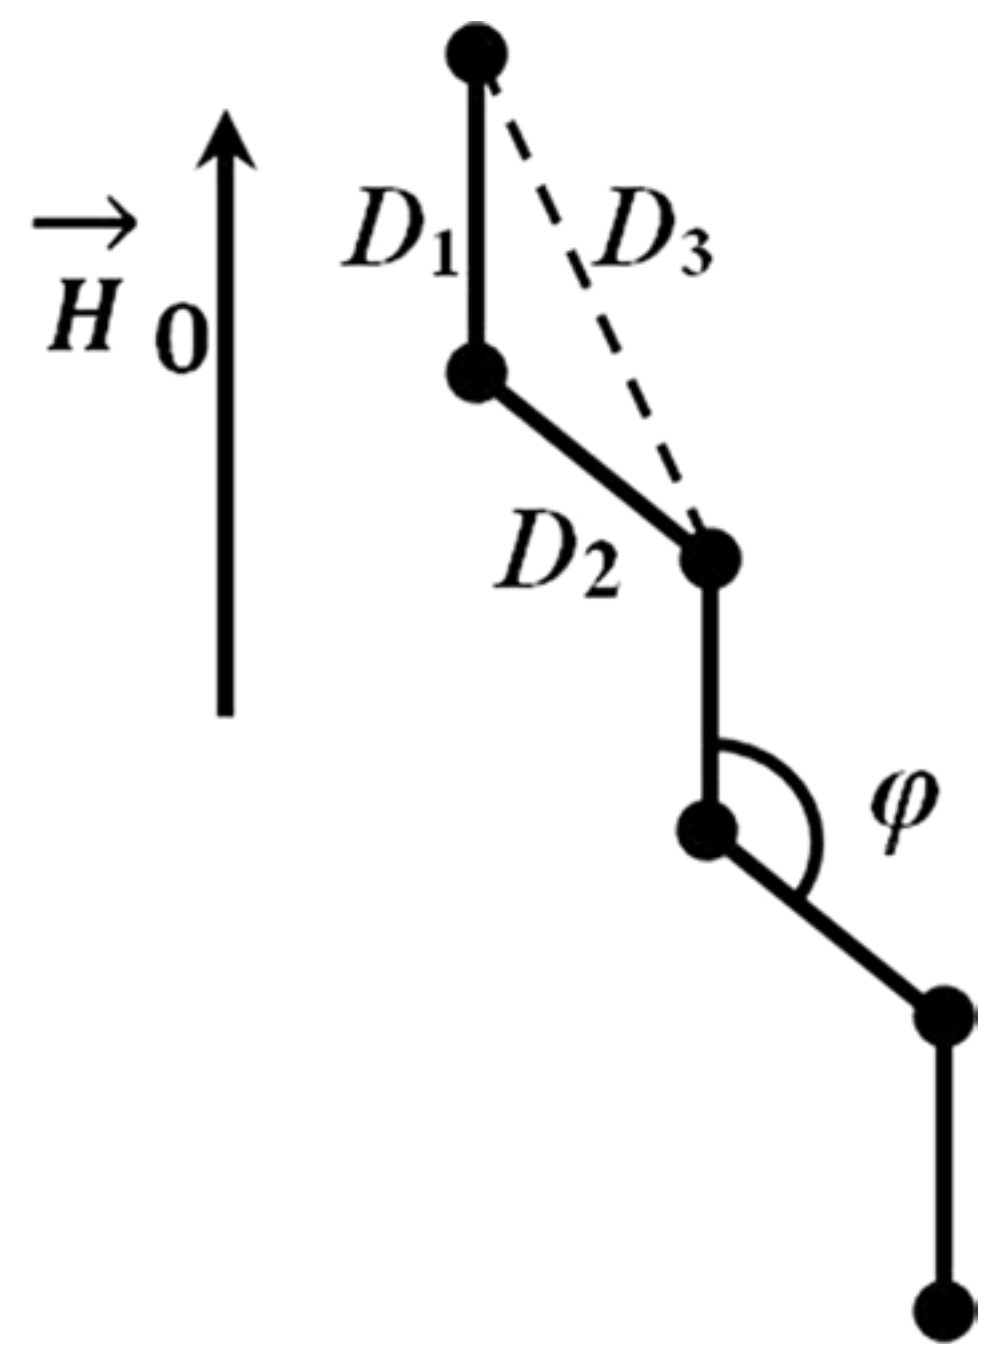
\includegraphics[width=0.5\textwidth]{model-zigzag-chain-schema.png}
%   \caption{Схема зигзагообзаной цепочки}
% \end{figure}
%
%     Константы взаимодействия
%         $$D_1=\dfrac{\gamma^2\hbar }{r^3}, $$
%         $$D_2 = D_1\dfrac{ 3\cos^2 \varphi -1 }{2} $$
%         $$D_3 = D_1 \dfrac{ 3\sin^2 \frac{\varphi}{2} -1}{16 \sin^3, \frac{\varphi}{2}}$$
%         где $\gamma$ - гиромагнитное отношение,
%         $\varphi$ - угол между соседними связями,
%         $r$ - расстояние между соседними спинами в цепочке.
%
%     Базовый случай это когда одна линия связи направлена вдоль поля. тогда констаты будет самой большой в доль поля.
%     Изменяя угол к полю мы можем получить как альтернированную цепочку так и однородную.
%     В приближении ближайших и следующих соседей, задача решается аналитически, но она
%     не дает полной картины. Поэтому мы решали данную систему численно.
%
%     \begin{figure}
%       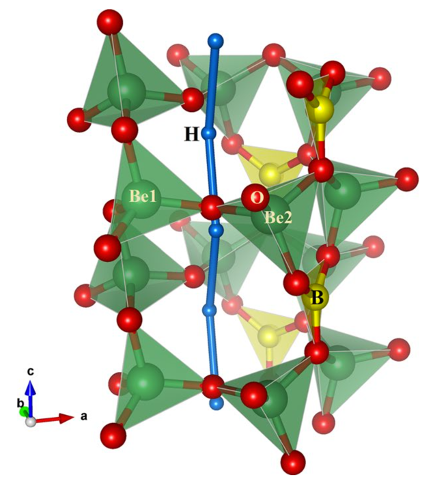
\includegraphics[width=0.85\textwidth]{model-zigzag-chain-hambergite-structure.png}
%       \caption{Hанопора со спин-несущих молекулами во внешнем сильном магнитном поле $\vec B$}
%     \end{figure}
%
%     Гамбергит $Be_2BO_3(OH)$
%         \begin{itemize}
%             \item Дипольное взаимодействия между ближайшими спинами протонов в цепи в 17 раз сильнее, чем со спинами окружающих цепей (в худшем случае).
%             \item Взаимодействия с остальными окружающими спинами по меньшей мере в 30 раз слабее.
%             \item Вклад дипольной связи между спинами в одной и той же цепи доминирует над остальными взаимодействиями.
%         \end{itemize}
%
%     В одномерных цепочках возникают когерентности только $\pm 2$ порядка
%     и следовательно дисперсия распределения будет небольшой
%     и мы не увидим запутанных кластеров.
%     Однако в альтернированная цепочке гамбергита возникают когерентности $\pm 4$ порядка
%     и следовательно можно использовать эту модель для исследования многочастичной запутанности.
%     The distance to these two protons is 4.49~\r{A}
%     The distance between a given chain and surrounding proton chains is at least 2.1 times larger than the distance between neighbors in the chain.
%

В предыдущей главе~\ref{chapter:manyparticle-entanglement-in-nanopore}
была подробно исследована многочастичная запутанность,
возникающая в МК эксперименте ЯМР в нанопоре,
и эта модель показала себя отличной площадкой
для исследования взаимодействия многих частиц.
Тем не менее одномерные модели~(см. раздел~\ref{sec:model-uniform-chain})
гораздо лучше изучены как теоретически,
так и экспериментально.
В частности в таких моделях изучены процессы
декогеренции~\cite{Bochkin2018},
передачи квантовых состояний~\cite{Lazarev2019, Feldman2020, Bochkin2022},
а также возникновения бинарной запутанности~\cite{Feldman2012, Lazarev2019}.
Ввиду такого широкого представления одномерных систем в литературе,
несомненно важно рассмотреть эти системы в контексте возникновения многочастичной запутанности.

% \section{Однородная цепочка}
% \subsection{Передача квантового состояния}
% \subsection{Температурная зависимость бинарной запутанности}

\section{Зигзагообразная цепочка}
В зигзагообразных цепочках в кристалле гамбергита в МК эксперименте ЯМР возникают когерентности плюс/минус четвертого порядка (см. раздел~\ref{sec:model-zigzag-chain}).
Данное обстоятельство является важным для исследования многоспиновой запутанности,
поскольку при этом используется второй момент распределения МК когерентностей ЯМР.

\begin{figure}[H]
    \centering
    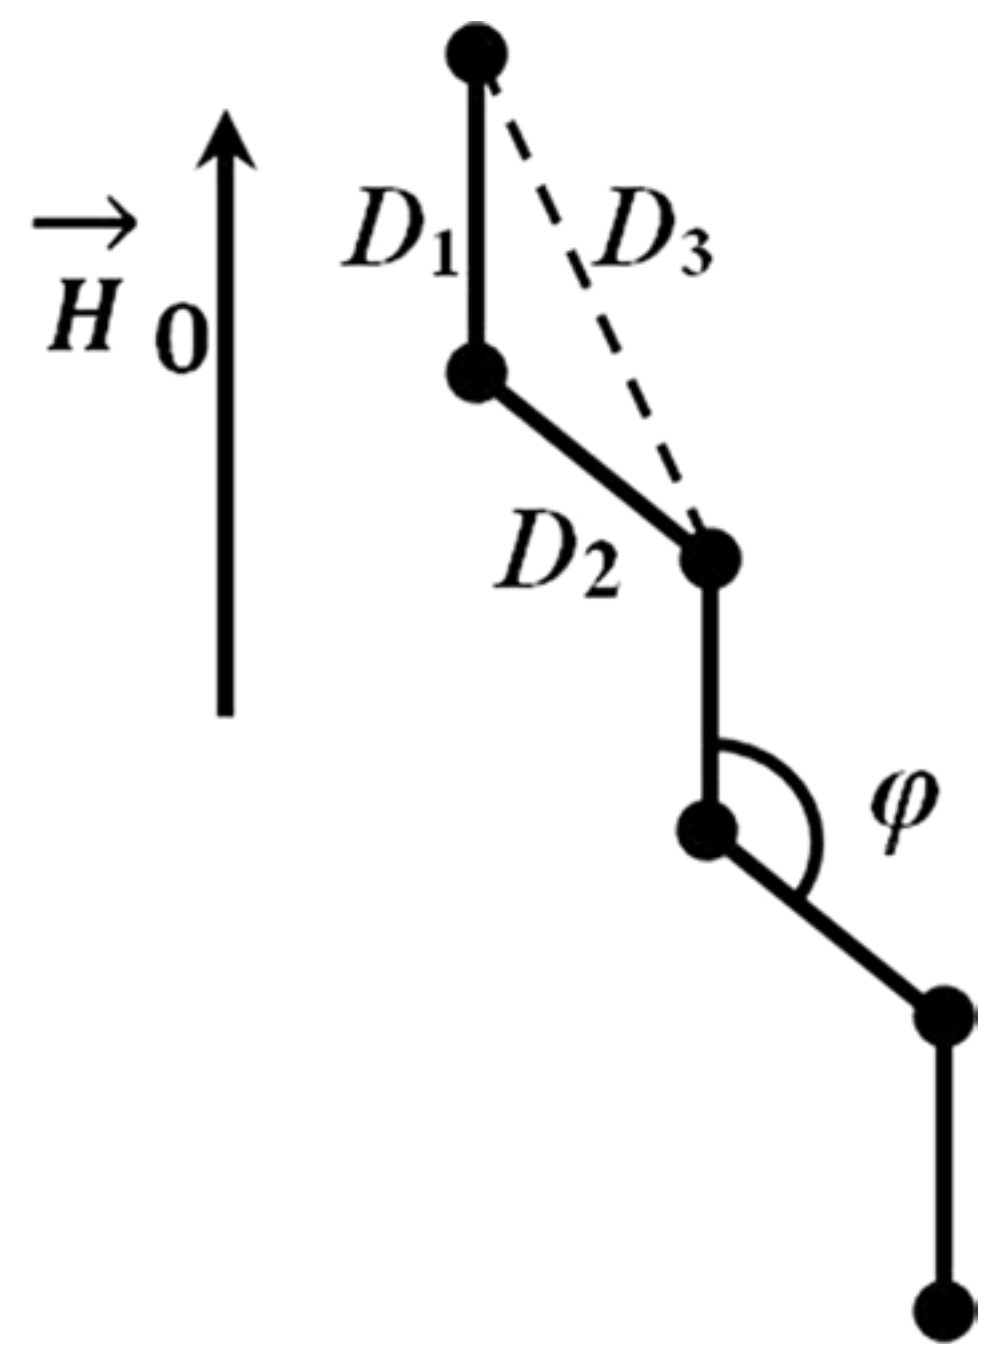
\includegraphics[width=0.3\textwidth]{model-zigzag-chain-schema}
    \caption{
      Зигзагообразная цепочка ядерных спинов.
      Нечетные звенья параллельны внешнему магнитному полю $\vec{\mathcal H}_0$,
      а $\varphi$ - угол между соседними звеньями.
      Константы связи $D_1$ и $D_2$ определяются уравнением~(\ref{eq:dipolaconstantsnearest}), а $D_3=D_{n, n+2},\, (n=1,2,...)$
      уравнением~(\ref{eq:dipolaconstantsnextnearest}).
    }
    \label{fig:model-zigzag-chain-schema}
\end{figure}

На рис.~\ref{fig:model-zigzag-chain-schema} схематично представлена
зигзагообразная цепочка ядерных спинов в сильном внешнем магнитным полем $\vec{\mathcal H}_0$.
Нечетные звенья цепочки параллельны внешнему магнитному полю $\vec{\mathcal H}_0$,
а $\varphi$ - угол между соседними звеньями.
Гамильтониан $H_\mathrm{MQ}$,
описывающий МК динамику ЯМР~(см. раздел~\ref{sec:mq-nrm-experiment}),
задается выражением~\cite{Doronin2000}
%
\begin{equation}\label{hmqnextnearest}
 H_\mathrm{MQ} = \sum_{i=1}^{N-1} D_{i, i+1}(I_i^{+}I_{i+1}^{+}+ I_i^{-}I_{i+1}^{-} )
   + \sum_{i=1}^{N-2} D_{i, i+2}(I_i^{+}I_{i+2}^{+}+ I_i^{-}I_{i+2}^{-} ) ,
\end{equation}
%
где $I_i^+$, $I_i^-$ --- это повышающей и понижающий операторы спинового углового момента спина с номером $i$,
и $N$ --- это количество ядерных спинов в цепочке.

Константы диполь-дипольного взаимодействия (ДДВ)
в зигзагообразной цепочке определяются выражениями~\cite{Abragam1982}
%
\begin{equation}\label{eq:dipolaconstantsnearest}
  D_{2n-1, 2n} = D_1 =\dfrac{\gamma^2\hbar }{r^3},
  \quad
  D_{2n, 2n+1} = D_2=\dfrac{\gamma^2\hbar }{2r^3}\p{3\cos^2 \varphi -1},
  \quad
  n=1,2\dots,
\end{equation}
где $\gamma$ --- это гиромагнитное отношение,
и $r$ --- это расстояние между ближайшими спинами в цепочке.
Также в гамильтониане учитываются взаимодействия со следующими соседями,
константа диполь-дипольного взаимодействия которых определяется как~\cite{Abragam1982}
%
\begin{equation}\label{eq:dipolaconstantsnextnearest}
  D_{n, n+2}=\dfrac{\gamma^2\hbar }{16r^3 \sin^3 \frac{\varphi}{2}}\p{3\sin^2 \frac{\varphi}{2} -1}.
\end{equation}
%
В частности, уравнения~(\ref{eq:dipolaconstantsnearest}),~(\ref{eq:dipolaconstantsnextnearest}) означают,
что для прямой спиновой цепочки, когда  $(\varphi=\pi)$,
константа дипольной связи для ближайших соседей в восемь раз больше,
чем константа дипольной связи между следующими ближайшими соседями.
Тем не менее при $\varphi=\frac{2\pi}{3}$ отношение констант связи
\begin{equation}
  \left|\dfrac{D_{2n, 2n+1}}{D_{2n-1, 2n+1}}\right| = \dfrac{3\sqrt{3}}{5},
\end{equation}
и, следовательно,
диполь-дипольные взаимодействия следующих ближайших соседей
существенны для МК динамики ЯМР при определённых ориентациях зигзагообразной спиновой цепочки
по отношению к направлению внешнего сильного магнитного поля.


\subsection{Температурная зависимость многочастичной запутанности}
Для исследования температурной зависимости многочастичной запутанности
в зигзагообразных цепочках
в этом разделе будет рассмотрена МК динамика ЯМР
на подготовительном периоде МК эксперимента ЯМР~(см. раздел~\ref{sec:mq-nrm-experiment})
с начальным термодинамически равновесным состоянием $\rho_\mathrm{eq}$.
Матрица плотности системы в начальный момент времени имеет вид:
\begin{equation}
  \rho(0, \beta)
  = \rho_\mathrm{eq}
  = \dfrac{e^{\frac{\hbar\omega_{0}}{kT} I_z}}{Z},
  = \dfrac{e^{\beta I_z}}{Z}
\end{equation}
где $Z = \tr{e^{\beta I_z}}$ --- статистическая сумма,
$\hslash$ и $k$ --- константы Планка и Больцмана,
$\omega_{0}$ --- частота Лармора,
$I_\mathrm{z}$ ---  оператор проекции полного углового спинового момента  на ось~$z$,
который направлен вдоль сильного внешнего магнитного поля.

Интенсивности приведенных МК когерентностей ЯМР определяются уравнением~\ref{eq:reduced-mq-coherences}~(см. раздел~\ref{sec:reduced-mq-coherences}).
Для $b=0.5$,
что соответствует температуре $T=4.8 \times 10^{-2}\,\mbox{K}$
при Ларморовской частоте $\omega_0=2\pi\times 500\times 10^6 \,\mbox{s}^{-1}$,
было обнаружено,
что неравенство~(\ref{eq:entanglement-criteria}) может быть выполнено только при $k=1$ для спиновых цепочек с $N=6$ и $N=8$.
Это означает, что в высокотемпературном случае~\cite{Doronin2019}
детектируется парная запутанность,
что согласуется с работой~\cite{Feldman2012}.

\begin{figure}[H]
  \begin{subfigure}[t]{0.49\textwidth}
    
\includegraphics[width=\textwidth]{m2-by-time-in-zigzag-chain-with-n6-beta10}				
    \caption{
      Зависимость нижней границы квантовой информации
      Фишера~$F_Q=2M_2(\tau, T)$
      от безразмерного времени~$D_1\tau$
      для зигзагообразной цепочки из 6 спинов
      при температуре $2.4\times 10^{-3}\,\mbox{K}$ $(b=10)$.
      В области выше горизонтальной линии $k=1$
      гарантировано существует как минимум парная запутанность.
      В области выше горизонтальной линии $k=5$
      гарантировано существует шестиспиновая запутанность.
    }
    \label{fig:fig3}
  \end{subfigure}
  \hfill
  \begin{subfigure}[t]{0.49\textwidth}
    
\includegraphics[width=\textwidth]{nent-by-n-b10}	
    \caption{
      Зависимость оценки максимального количества запутанных спинов $N_{ent}$ от длины цепочки при темперутуре $2.4\times 10^{-3}\,\mbox{K}$.
    }
    \label{fig:fig4}
  \end{subfigure}
  \caption{}
\end{figure}

Зависимости многоспиновой запутанности от длины цепочки $N$ и температуры исследованы для спиновых цепочек с $4\leqslant N \leqslant 12$.
Временная эволюция нижней границы квантовой информации Фишера,
соответствующая  удвоенному второму моменту распределения интенсивностей МК когерентностей для шестиспиновой цепочки представлена на рис.~\ref{fig:fig3} при температуре $2.4\times 10^{-3}\,\mbox{K}$ $(b=10)$.
На рис.~\ref{fig:fig3} видна полоса,
в которой неравенство~(\ref{eq:entanglement-criteria}) может быть удовлетворено при $1\leqslant k \leqslant 5$.
Таким образом, существует многоспиновая запутанность в спиновых кластерах, состоящих из 2-6 спинов при температуре $2.4\times 10^{-3}\,\mbox{K}$.
Зависимость оценки максимального количества запутанных спинов от длины цепи приведена на рис.~\ref{fig:fig4} при температуре $2.4\times 10^{-3}\,\mbox{K}$.

\begin{figure}[H]
  \begin{subfigure}[t]{0.49\textwidth}
    
\includegraphics[width=\textwidth]{m2-by-time-in-zigzag-chain-with-n8-beta1}				
    \caption{
      При температуре $2.4\times 10^{-2}\,\mbox{K}$
      в области ограниченной горизонтальными линиями $k=1$ и $k=2$
      присутствует как минимум парная запутанность.
    }
    \label{fig:fig5}
  \end{subfigure}
  \hfill
  \begin{subfigure}[t]{0.49\textwidth}
    
\includegraphics[width=\textwidth]{m2-by-time-in-zigzag-chain-with-n8-beta10}				
    \caption{
       При температуре $1.2\times 10^{-3}\,\mbox{K}$
       в области ограниченной горизонтальными линиями $k=2$ и $k=4$
       наблюдается как минимум трехчастичная запутанность.
    }
    \label{fig:fig6}
  \end{subfigure}
  \caption{
    Временная эволюция нижней границы информации Фишера~$F_Q=2M_2(\tau, T)$
    от безразмерного времени~$D_1\tau$
    в восьмиспиновой зигзагообразной цепочке.
  }
\end{figure}

Временная эволюция восьмиспиновой зигзагообразной цепочки представлена при $T=2.4\times 10^{-2}\,\mbox{K}$ (рис.~\ref{fig:fig5}) и $T=1.2\times 10^{-2}\,\mbox{K}$ (рис.~\ref{fig:fig6}).  Видно, что при температуре $T=2.4\times 10^{-2}\,\mbox{K}$ возникают многоспиновые запутанные кластеры, состоящие из двух или трех спинов, а при температуре $T=1.2\times 10^{-2}\,\mbox{K}$ возникают кластеры с $2\leqslant k \leqslant 5$.
Число запутанных спинов увеличивается с понижением температуры.

\begin{figure}[H]
  \centering
  
\includegraphics[width=0.6\textwidth]{nent-by-beta-n8-n6}				
  \caption{
    Зависимость оценки максимального числа запутанных спинов от обратной температуры $b$
    для зигзагообразной цепочки,
    состоящей из шести и восьми спинов.
    }
    \label{fig:fig7}
\end{figure}

Зависимость числа запутанных спинов от температуры для зигзагообразных цепочек,
состоящих из шести или восьми спинов, приведена на рис.~\ref{fig:fig7}.
% В этих цепочках почти все спины запутаны при низких температурах.
Также как и в случае системы эквивалентных спинов,
при низких температурах почти все спины в цепочке запутанны.
% Результаты получены на небольшом интервале времени,
% поэтому эффектами декогеренции можно пренебречь.


% The creation of entangled clusters in the considered zigzag chains is limited by weak DDIs of remote spins.  Accordingly, that process requires a large time interval. Practically, the role of decoherence gets very important in that case.  We note also that the analysis of the inequality \eqref{inequalityforfq} shows that an increase in chain length does not result in an increase of the number of the entangled spins even at long times. Indeed, we can rewrite \eqref{inequalityforfq} in the approximate simple form
% \begin{equation}\label{inequalityforfq2}
% F_Q>k N.
% \end{equation}
% In order to estimate the Fisher information we use the Gaussian approximation for the distribution of the intensities of MQ coherences \cite{baum}
% \begin{equation}\label{gaussaprox}
% J(\tau, T)=\dsfrac{1}{\sqrt{\pi N_c(T)}} \exp\ls{-\frac{n^2}{N_c(T)}}\rs,
% \end{equation}
% where $N_c(T)$ is the number of the correlated spins which are responsible for the creation of the MQ coherence profile. Since twice the second moment $2M_2(\tau, T)$ is a lower bound on the quantum Fisher information $F_Q$ \cite{toth, pezze} one can find from Eq. \eqref{gaussaprox} that
% \begin{equation}\label{qfisheinf}
% F_Q=N_c(T).
% \end{equation}
% Since $N\geqslant N_c(T)$, one can conclude that in the Gaussian model \cite{baum} only two-spin entanglement is possible.
%
% Numerical calculations for the zigzag spin chain yield similar results. We find that the Fisher information depends only weakly on the number of spins. It means (see Eq. \eqref{inequalityforfq2}) that the number of the entangled spins decreases when $N$ increases. We have found that in the zigzag six-spin system all six spins can be entangled. On the contrary, only three spins are entangled in the zigzag ten-spin system.
%
% Finally, the number of the entangled spins for the zigzag chain with $4\leqslant N\leqslant 12$ increases with decreasing temperature.


\section{Выводы}
В этом разделе была исследована многочастичная запутанность
возникающая на подготовительном периоде МК эксперимента ЯМР
в зигзагообразной цепочке ядерных спинов.
Несмотря на то, что в одномерных системах
создание запутанных кластеров ограничено слабыми ДДВ удаленных спинов,
удалось показать что качественное поведение температурной зависимости многочастичной запутанности
в зигзагообразной цепочке совпадает с поведением в системе эквивалентных спинов.
%Несмотря на то, что одномерные системы демонстрируют
%более скромные оценки количества запутанных частиц
%из-за отсутствия сильных дальнодействующих связей,
%можно заключить,
%что качественное поведение температурной зависимости многочастичной запутанности
%совпадает с поведением в системе эквивалентных спинов.
Более того, полученные результаты исследования запутанности
соответствуют результатам, представленным в литературе.
Таким образом, можно заключить,
что разработанный в данной диссертации метод
является мощным инструментом для исследования многочастичной запутанности в любой системе.
\chapter{Измерение информации Вигнера-Янасе в МК эксперименте ЯМР}
\label{chapter:wyi-mesuarement}

% PLA-2021

В разделе~\ref{sec:manyparticle-entanglement-criteria} был обсужден критерий многочастичной запутанности
в терминах обобщенной информации.
В свою очередь в разделах~\ref{sec:quantum-fisher-information}~и~\ref{sec:skew-wigner-yanase-information}
было показано,
что в качестве такой обобщённой меры информации могут выступать
квантовая информация Фишера и косая информация Вигнера-Янасе.
Тем не менее в прошлых разделах многочастичная запутанность была исследована исключительно
на основе квантовой информации Фишера.
Главной причиной такого выбора является тот факт,
что нижняя граница квантовой информации Фишера может быть измерена в МК эксперимента ЯМР~(см.  раздел~\ref{sec:quantum-fisher-information-mesuarement-at-high-temperature}),
и, следовательно, многочастичная запутанность может быть исследована экспериментально.
В этой главе будет продемонстрировано,
что и косая информация Вигнера-Янасе связана с
со вторым моментом МК спектра ЯМР,
а также проведено сравнение оценок многоспиновой запутанности
на основе косой информации Вигнера-Янаса и квантовой информации Фишера.



\section{Связь косой информации и второго момента МК спектра ЯМР}
\label{sec:wyi-mesuarement}

Для прояснения связи косой информации Вигнера-Янаса и
второго момента интенсивностей МК когерентностей ЯМР,
ниже будет получено выражение для косой информации
на подготовительном периоде МК эксперимента ЯМР~(см. раздел~\ref{sec:mq-nrm-experiment})
с начальным термодинамически равновесным состоянием $\rho_\mathrm{eq}$.
Матрица плотности системы в начальный момент времени имеет вид:
\begin{equation}
  \rho(0, \beta)
  = \rho_\mathrm{eq}
  = \dfrac{e^{\frac{\hbar\omega_{0}}{kT} I_z}}{Z},
  = \dfrac{e^{\beta I_z}}{Z},
\end{equation}
где $Z = \tr{e^{\beta I_z}}$ --- статистическая сумма,
$\hslash$ и $k$ --- константы Планка и Больцмана,
$\omega_{0}$ --- частота Лармора,
$I_\mathrm{z}$ ---  оператор проекции полного углового спинового момента  на ось~$z$,
который направлен вдоль сильного внешнего магнитного поля.
Эволюционная матрица плотности $\rho(\tau,\beta)$ на подготовительном периоде
под действием стационарного гамильтониана $H_\mathrm{MQ}$
может быть получена из уравнения Лиувилля,
которое имеет вид
%
\begin{equation}\label{eq:rho-eval}
  \rho(\tau,\beta)
  = V^+(\tau) \rho(0, \beta) V(\tau)
  = V^+(\tau) \frac{e^{\beta I_z}}{Z} V(\tau),
\end{equation}
где $V(\tau) = e^{iH_\mathrm{MQ}\tau}$
--- это оператор эволюции.

Косая информация Вигнера-Янасе определяется выражением~(см. раздел~\ref{sec:skew-wigner-yanase-information})
%
\begin{equation}\label{eq:wyi}
  I_{WY}(\rho(\tau,\beta),I_z)
  = -\frac{1}{2} Tr([\sqrt{\rho(\tau,\beta)},\sigma_z])^2
  = -2 Tr([\sqrt{\rho(\tau,\beta)},I_z])^2,
\end{equation}
%
где $\sigma_z=2I_z$ --- это оператор Паули.
Интригующей особенностью определения косой информации Вигнера-Янасе
является наличие корня из матрицы плотности.
Корень из матрицы плотности $\rho(\tau,\beta)$ определяется выражением
%
\begin{equation}\label{eq:rho-eval-sqrt}
  \sqrt{\rho(\tau,\beta)}
  = \sqrt{V^+(\tau)\frac{e^{\beta I_z}}{Z}V(\tau)}
  = V^+(\tau) \frac{e^{\frac{\beta}{2}I_z}}{\sqrt{Z}}V(\tau),
\end{equation}
которое может быть проверено простым вычислением:
\begin{equation}\label{eq:18}
   \sqrt{\rho}\sqrt{\rho}
   = V^+(\tau)\frac{e^{\frac{\beta}{2}I_z}}{\sqrt{Z}}
     V(\tau)V^+(\tau)\frac{e^{\frac{\beta}{2}I_z}}{\sqrt{Z}}V(\tau)
   = V^+(\tau)\frac{e^{\beta I_z}}{Z}V(\tau)
   = \rho(\tau,\beta).
\end{equation}
%
Выражение~(\ref{eq:rho-eval-sqrt}) для корня эволюционной матрицы плотности отражает интересное физическое свойство.
В действительности можно отказаться от корня
в выражении~(\ref{eq:wyi}) косой информации Вигнера-Янасе
и перейти к рассмотрению системы при вдвое большей температуре
с матрицей плотности $\rho\p{\tau,\frac \beta 2}$.
Для анализа вкладов отдельных МК когерентностей ЯМР в эволюционную матрицу плотности
$\rho(\tau,\frac \beta 2)$ можно представить ее в виде ряда~\cite{Feldman1996}
%
\begin{equation}\label{eq:}
  \rho\p{\tau,\frac \beta 2} = \sum_n \rho_{n}\p{\tau,\frac \beta 2},
\end{equation}
%
Тогда коммутатор в выражении~(\ref{eq:wyi}) можно переписать как
%
\begin{equation} \label{eq:19}
    \left[I_z,\sqrt{\rho(\tau,\beta)}\right]
    = \left[I_z, \sum_k \rho_k \left(\tau, \frac{\beta}{2}\right)\right]
    = \sum_k k\rho_k \left(\tau, \frac{\beta}{2}\right),
\end{equation}
%
и
%
\begin{equation} \label{eq:20}
	Tr\left[I_z,\sqrt{\rho(\tau,\beta)} \right]^2
	= Tr\left\{\sum_{k,k'}kk'
		\rho_k\left(\tau,\frac{\beta}{2}\right)
		\rho_{k'}\left(\tau,\frac{\beta}{2}\right)
	\right\}
	= \sum_k k^2 J_k\left(\tau,\frac{\beta}{2}\right).
\end{equation}
%
В итоге, получаем выражение для косой информации Вигнера-Янасе
через второй момент интенсивности МК когерентностей ЯМР
%
\begin{equation}\label{eq:wyi-via-second-moment}
    I_{WY}\left(\rho(\tau, \beta), I_z\right)
    = 2\sum_k k^2 J_k\left(\tau, \frac{\beta}{2}\right)
    = 2M_2\left(\tau, \frac{\beta}{2}\right).
\end{equation}
%
Таким образом, мы получаем важное наблюдение.
Если спиновая система исследуется с помощью МК ЯМР при температуре $T\sim\beta^{-1}$,
то косая информация Вигнера-Янаса равна удвоенному второму моменту
распределения интенсивностей когерентностей МК ЯМР при температуре $2T \sim 2\beta^{-1}$
в любой момент времени эволюции спиновой системы на подготовительном периоде МК эксперимента ЯМР.

Полученное равенство~(\ref{eq:wyi-via-second-moment}) позволяет экспериментально исследовать
косую информацию Вигнера-Янасе в МК эксперименте ЯМР.
В частности, по аналогии с квантовой информации Фишера
может быть исследована многочастичная запутанность (см. следующий раздел~\ref{sec:qfi-wyi-entanglement-comparison}).


\section{Сравнение оценок количества запутанных частиц}
\label{sec:qfi-wyi-entanglement-comparison}

В разделах~\ref{sec:quantum-fisher-information}~и~\ref{sec:skew-wigner-yanase-information} обсуждалось,
что квантовая информация Фишера и косая информация Вигнера-Янасе
могут быть независимо использованы для оценки количества запутанных частиц.
Ввиду результатов, полученных в разделах~\ref{sec:reduced-mq-coherences}~и~\ref{sec:wyi-mesuarement},
можно заключить,
что обе информации могут быть измерены в МК эксперименте ЯМР.
Более того, в отличие от квантовой информации Фишера,
косая информация Вигнера-Янасе может быть измерена точно.
Следовательно, возникает естественная мотивация провести сравнение
этих информаций в контексте исследования многочастичной запутанности.
Результаты такого сравнения представлены в данном разделе.

% \begin{figure}[H]
% 	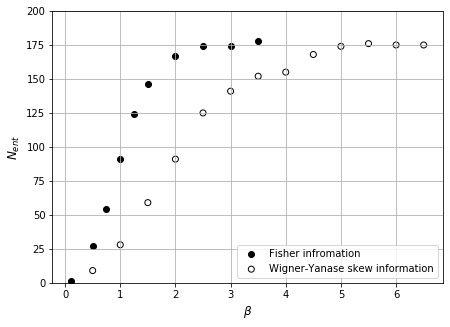
\includegraphics[width=0.95\linewidth]{nanopora_entangled_spins_by_temp}
% 	\caption{
% 		Зависимость оценки числа запутанных спинов в системе от обратной температуры $\beta = \frac{\pi \omega_0}{kT}$
% 		в нанопоре.
% 		Черные круги --- результаты полученные на основе квантовой информации Фишера.
% 		Белые круги --- результаты полученные на основе косой информации Вигнера-Янасе.
% 	}
% 	\label{fig:2}
% \end{figure}
%
% \begin{figure}[H]
% 	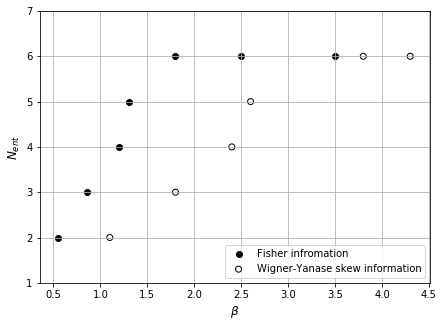
\includegraphics[width=0.95\linewidth]{zigzag_entangled_spins_by_temp}
% 	\caption{
% 		Зависимость оценки числа запутанных спинов  $N_\mathrm{ent}$
% 		от параметра обратной температуры $\beta = \frac{\pi \omega_0}{kT}$
% 		в зигзагообразной цепочке, состоящей из шести спинов.
% 		Черные круги --- результаты полученные на основе квантовой информации Фишера.
% 		Белые круги --- результаты полученные на основе косой информации Вигнера-Янасе.
% 	}
% 	\label{fig:3}
% \end{figure}

\begin{figure}[H]
  \centering
  \begin{subfigure}[t]{0.49\textwidth}
    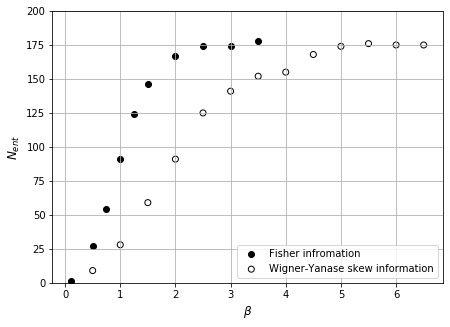
\includegraphics[width=\linewidth]{nanopora_entangled_spins_by_temp}
	\caption{
		Нанопора заполненная спин-несущими частицами.
	}
	\label{fig:qfi-wyi-comparison-nanopora}
  \end{subfigure}
  \hfill
  \begin{subfigure}[t]{0.49\textwidth}
    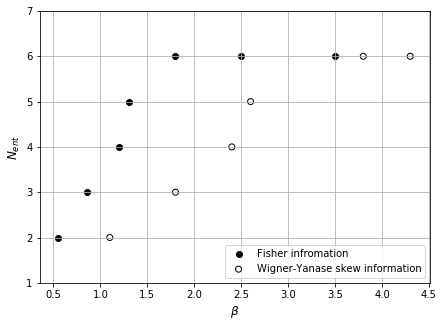
\includegraphics[width=\linewidth]{zigzag_entangled_spins_by_temp}
	\caption{
		Зигзагообразная цепочка, состоящей из шести спинов.
	}
	\label{fig:qfi-wyi-comparison-zigzag-chain}
  \end{subfigure}
  \caption{
    Зависимость оценки снизу числа запутанных спинов  $N_\mathrm{ent}$
	от параметра обратной температуры $\beta = \frac{\pi \omega_0}{kT}$
	Черные круги --- результаты полученные на основе квантовой информации Фишера.
	Белые круги --- результаты полученные на основе косой информации Вигнера-Янасе.
  }
  \label{fig:qfi-wyi-comparison}
\end{figure}

Величины квантовой информации Фишера~$I_\mathrm{F}(\rho(\tau,\beta),I_z)$ и косой информации Вигнера-Яанасе~$I_{WY}(\rho(\tau,\beta),I_z)$
связаны с количеством запутанных частиц в системе (см. раздел~\ref{sec:manyparticle-entanglement-criteria}).
Если величина информации превышает значение $mk^2 + (N - mk)^2$,
где $k, m$ целые числа и $m$ --- это целая часть $N/k$,
тогда гарантируется,
что в системе как минимум $k+1$ частиц связаны в одно несепарабельное состояние.

В разделе~\ref{sec:qfi-wyi-comparison} было получено следующее неравенство
для квантовой информации Фишера и косой информации Вигнера-Янасе:
%
\begin{equation} \label{eq:qfi-wyi-inequality}
    I_{WY}\left(\rho(\tau,\beta), I_z\right)
    \leq I_F\left(\rho(\tau,\beta), I_z\right)
    \leq 2I_{WY}\left(\rho(\tau,\beta), I_z\right).
\end{equation}
%
Неравенство~(\ref{eq:qfi-wyi-inequality}) позволяет надеяться,
что полученные результаты для оценки числа запутанных спинов не будут значительно отличаться.

На Рис.~\ref{fig:qfi-wyi-comparison} представлены результаты зависимости
оценки снизу количества запутанных частиц в системе от обратной температуры $\beta$.
Оценки количества запутанных частиц были полученных на основе квантовой информации Фишера и косой информации Вигнера-Янасе.
Величины обеих информаций были вычислены через второй момент распределения МК когерентностей ЯМР~(cм.
разделы~\ref{sec:reduced-mq-coherences}~и~\ref{sec:wyi-mesuarement}).
На Рис.~\ref{fig:qfi-wyi-comparison-nanopora} сравнение проведено для модели несферической нанопоры,
заполненной газом спин-несущих атомов (например, ксеноном) или молекул в сильном внешнем магнитном поле~(см. раздел~\ref{sec:model-equivalent-spins}).
Расчеты второго момента $M_2(\tau, \beta)$ были сделаны по аналогии с разделом~\ref{sec:nanopora-thermodynamic-equilibrium} для системы из 201 спина.
На Рис.~\ref{fig:qfi-wyi-comparison-zigzag-chain} сравнение проведено
для модели зигзагообразной цепочки ядерных спинов в кристалле гамбергита~(см. раздел~\ref{sec:model-zigzag-chain}).
Расчеты второго момента $M_2(\tau, \beta)$ были сделаны по аналогии с главой~\ref{chapter:manayparticle-entantlement-in-zigzag-chain}

% \section{Обобщения косой информации}
% \begin{align}
%     I_{WY}\left( \rho(t, T), I_z \right) & = 2\sum\limits_k k^2 J_k(t, 2T) = 2M_2(t, 2T) \\
%     I_{WYG}\left( \rho(t, T), I_z \right) &  = -2 \tr{\left[\rho(t, T), I_z\right]} = 2M_2(t, T) \\
%     I_{WYD} \left( \rho(t, T), I_z \right) &  = -2 \mathrm{Tr} \left\{
%         \left[\rho^\alpha, I_z \right] \left[\rho^{1 - \alpha}, I_z \right]
%     \right\}
% \end{align}

\section{Выводы}
Косая информация Вигнера-Янасе, так же как и информация Фишера,
является одной из важнейших мер в теории квантовой информации.
Полученный в этом разделе результат открывает множество возможностей
экспериментального исследования косой информации в различных системах.
В частности, она может быть применена для экспериментального исследования многочастичной запутанности.
Подобные исследования многочастичной запутанности требуют крайне низких температур $<10^{-3}$~K.
В этом случае информация Вигнера-Янасе имеет существенное преимущество перед информацией Фишера,
так как измерение первой для системы с температурой $T$
может быть проведено на установке с вдвое большей температурой $2T$.
\chapter*{Заключение}
\addcontentsline{toc}{chapter}{Заключение}
\chapter*{Заключение}
\addcontentsline{toc}{chapter}{Заключение}

\chapter*{Благодарности}
И.Д. Лазарев выражает благодарность научному руководителю профессору Э.Б. Фельдману
и коллегам
Г.А. Бочкину,
С.Г. Васильеву,
С.И. Доронину,
А.И. Зенчуку,
Е.И. Кузнецовой,
и А.H. Пыркову.

И.Д. Лазарев выражает признательность за поддержку Фонду развития теоретической физики и математики ``Базис'' (№19-1-5-130-1).

Работа выполнена при поддержке фонда Министерства Науки и Высшего Образования Российской Федерации (№075-15- 2020-779) и частично (№075-15-2020-788).

\bibliographystyle{unsrt}
\bibliography{bibliography}
\end{document}
